\documentclass[hidelinks, paper=a4, fontsize=13pt]{report}
\usepackage{graphicx}
\usepackage[utf8]{inputenc}
\usepackage{color}
\usepackage{textcomp}
\usepackage{charter}
\usepackage[T1]{fontenc}
\usepackage[top=1in, bottom=1in, left=0.7in, right=0.7in]{geometry}
\usepackage[frenchb]{babel}
\usepackage{caption}
\usepackage[table,xcdraw]{xcolor}
\usepackage{pdfpages}
\usepackage{sectsty} 
\allsectionsfont{\normalfont\scshape}
\usepackage{array, booktabs}
\usepackage{supertabular}
\usepackage{multirow}
\usepackage{hyperref}
\hypersetup{colorlinks=false,linktoc=all}
\usepackage{fancyhdr} 
\usepackage{eurosym}
\pagestyle{fancy} 
\fancyhead{} 
\fancyfoot[L]{\small{24 heures de l'INSA - 2019}} 
\fancyfoot[C]{\small\hyperref[table_matiere]{Raccourci vers la table des matières}}
\fancyfoot[R]{\thepage}
\renewcommand{\headrulewidth}{0pt}
\renewcommand{\footrulewidth}{0pt}
\setlength{\headheight}{13.6pt}
\setcounter{secnumdepth}{9}
\setlength\parindent{0pt}

\begin{document}

\begin{center}
\rule[0.5ex]{\linewidth}{2pt}\vspace*{-\baselineskip}\vspace*{4.2pt}
\rule[0.5ex]{\linewidth}{1pt}\\[\baselineskip]
\huge Dossier de sécurité\\24 heures de l'INSA - 45\up{e} édition \\[4mm]
{\Large \textit{17, 18 et 19 mai 2019}}\\
\rule[0.5ex]{\linewidth}{1pt}\vspace*{-\baselineskip}\vspace{3.2pt}
\rule[0.5ex]{\linewidth}{2pt}\\
\vspace{20mm}
\end{center}
{\large Contacts:}\\
\vspace{3.5mm}
{\large\textsc{\\
Ludovic GIRY – Président\\}
ludovic.giry@24heures.org  – 06 58 09 61 40\\\\\textsc{
Arthur SAUNIER – Resposable Sécurité\\}
arthur.saunier@24heures.org – 06 25 53 25 79\\\\\textsc{
Loïc JEGOU – Responsable Sécurité\\}
loic.jegou@24heures.org  – 06 58 17 07 39\\\\}\\
\vspace{20mm}

   \begin{minipage}[c]{.46\linewidth}

\includegraphics[scale=1]{Annexes/Images/logo24h.jpg}\\
   \end{minipage} \hfill
   \begin{minipage}[c]{.46\linewidth}

\includegraphics[scale=1]{Annexes/Images/villeurnoir}\\
   \end{minipage}
\begin{flushright}
\vspace{15mm}


{\large\textsc{Janvier 2019}}

\vspace{15mm}


\end{flushright}

\newpage

%------------------------------------------------------------------------------------------------------
%PRESENTATION
%------------------------------------------------------------------------------------------------------

\chapter{Présentation}
\section{Contacts}
\label{refTelPC}

\textbf{1. PC sécurité}\\
Adresse : Bibliothèque Marie Curie, avenue Jean Capelle Ouest, INSA LYON\\
Ligne principale : \textbf{04 28 29 63 82}\\
Ligne secondaire : \textbf{04 72 43 70 70}\\\\

\textbf{2. Responsables sécurité}\\
Ludovic Giry (président) : \textbf{06 58 09 61 40}\\
Arthur Saunier : \textbf{06 25 53 25 79}\\
Loïc Jegou : \textbf{06 58 17 07 39}\\
\\

\textbf{3. DPS – Croix Rouge}\\
Responsable de dispositif, Loïc Morcel : \textbf{06 83 26 24 01}\\\\

\textbf{4. PCO (Poste de Commandement Opérationnel}\\
Adresse : Bibliothèque Marie Curie, avenue Jean Capelle Ouest, INSA LYON\\
\textit{Ce PC n’est armé qu'en cas de déclenchement du plan d'évacuation de niveau 3 ou du plan NOVI.\\\\
}Lignes d’urgence : 			\textbf{04 72 43 72 01   à 	04 72 43 72 04}\\
Fax : 					\textbf{04 72 43 72 05}\\

\textbf{5. Société de sécurité}\\
Responsable STAFF Sécurité, Jean-Christophe Bel : \textbf{06 98 16 40 50}\\
 
\newpage

\section{Organisateurs}
\label{refTelOrgas}

\tabletail{\hline}


\begin{supertabular}{|m{1.33cm}|m{1.33cm}|m{1.33cm}|m{1.33cm}|m{1.33cm}|m{1.33cm}|m{1.33cm}|m{1.33cm}|m{1.33cm}|m{1.33cm}|m{1.33cm}|m{1.33cm}|}
\shrinkheight{1cm} 

\hline
\multicolumn{12}{|m{16cm}|}{}\\
\multicolumn{12}{|c|}{\bf Responsables Sécurité}\\
\multicolumn{12}{|c|}{securite@24heures.org}\\
\multicolumn{4}{|m{5.33cm}}{\rule{0pt}{2ex}} & \multicolumn{4}{m{5.33cm}}{} & \multicolumn{4}{m{5.33cm}|}{} \\
\multicolumn{4}{|c}{\centering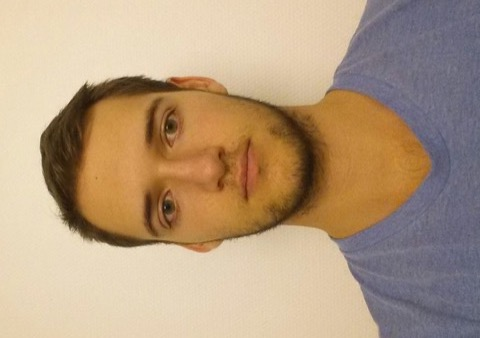
\includegraphics[height=4cm]{Annexes/Trombi_orgas/Orga_secu_1}}  & \multicolumn{4}{c}{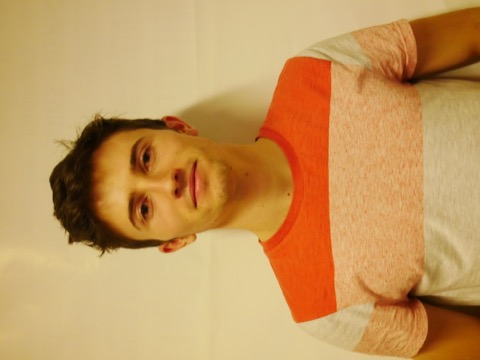
\includegraphics[height=4cm]{Annexes/Trombi_orgas/Orga_secu_2}} & \multicolumn{4}{c|}{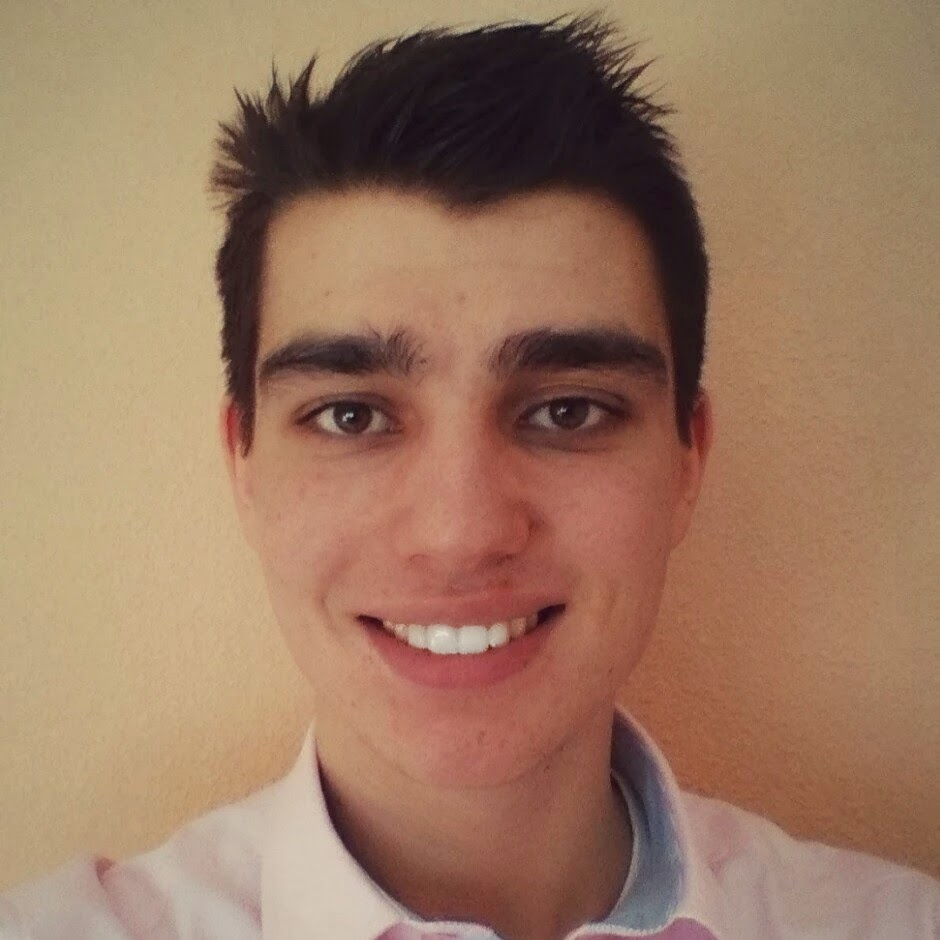
\includegraphics[height=4cm]{Annexes/Trombi_orgas/Orga_secu_3}} \\
\multicolumn{4}{|c}{Ludovic GIRY}  & \multicolumn{4}{c}{Arthur SAUNIER} & \multicolumn{4}{c|}{Loïc JEGOU} \\
\multicolumn{4}{|c}{06 58 09 61 40}  & \multicolumn{4}{c}{06 25 53 25 79} & \multicolumn{4}{c|}{06 58 17 07 39} \\

\hline

\multicolumn{3}{|m{4cm}|}{} & \multicolumn{3}{m{4cm}|}{} & \multicolumn{3}{m{4cm}}{} & \multicolumn{3}{m{4cm}|}{}\\
\multicolumn{3}{|c|}{\bf Trésorière} & \multicolumn{3}{c|}{\bf Responsable Billetterie} & \multicolumn{6}{c|}{\bf Responsables Barriere}\\
\multicolumn{3}{|c|}{tresorier@24heures.org} & \multicolumn{3}{c|}{billetterie@24heures.org} & \multicolumn{6}{c|}{logistique.barrieres@24heures.org}\\
\multicolumn{3}{|c|}{\rule{0pt}{2ex}} & \multicolumn{3}{c|}{} & \multicolumn{6}{c|}{} \\
\multicolumn{3}{|c|}{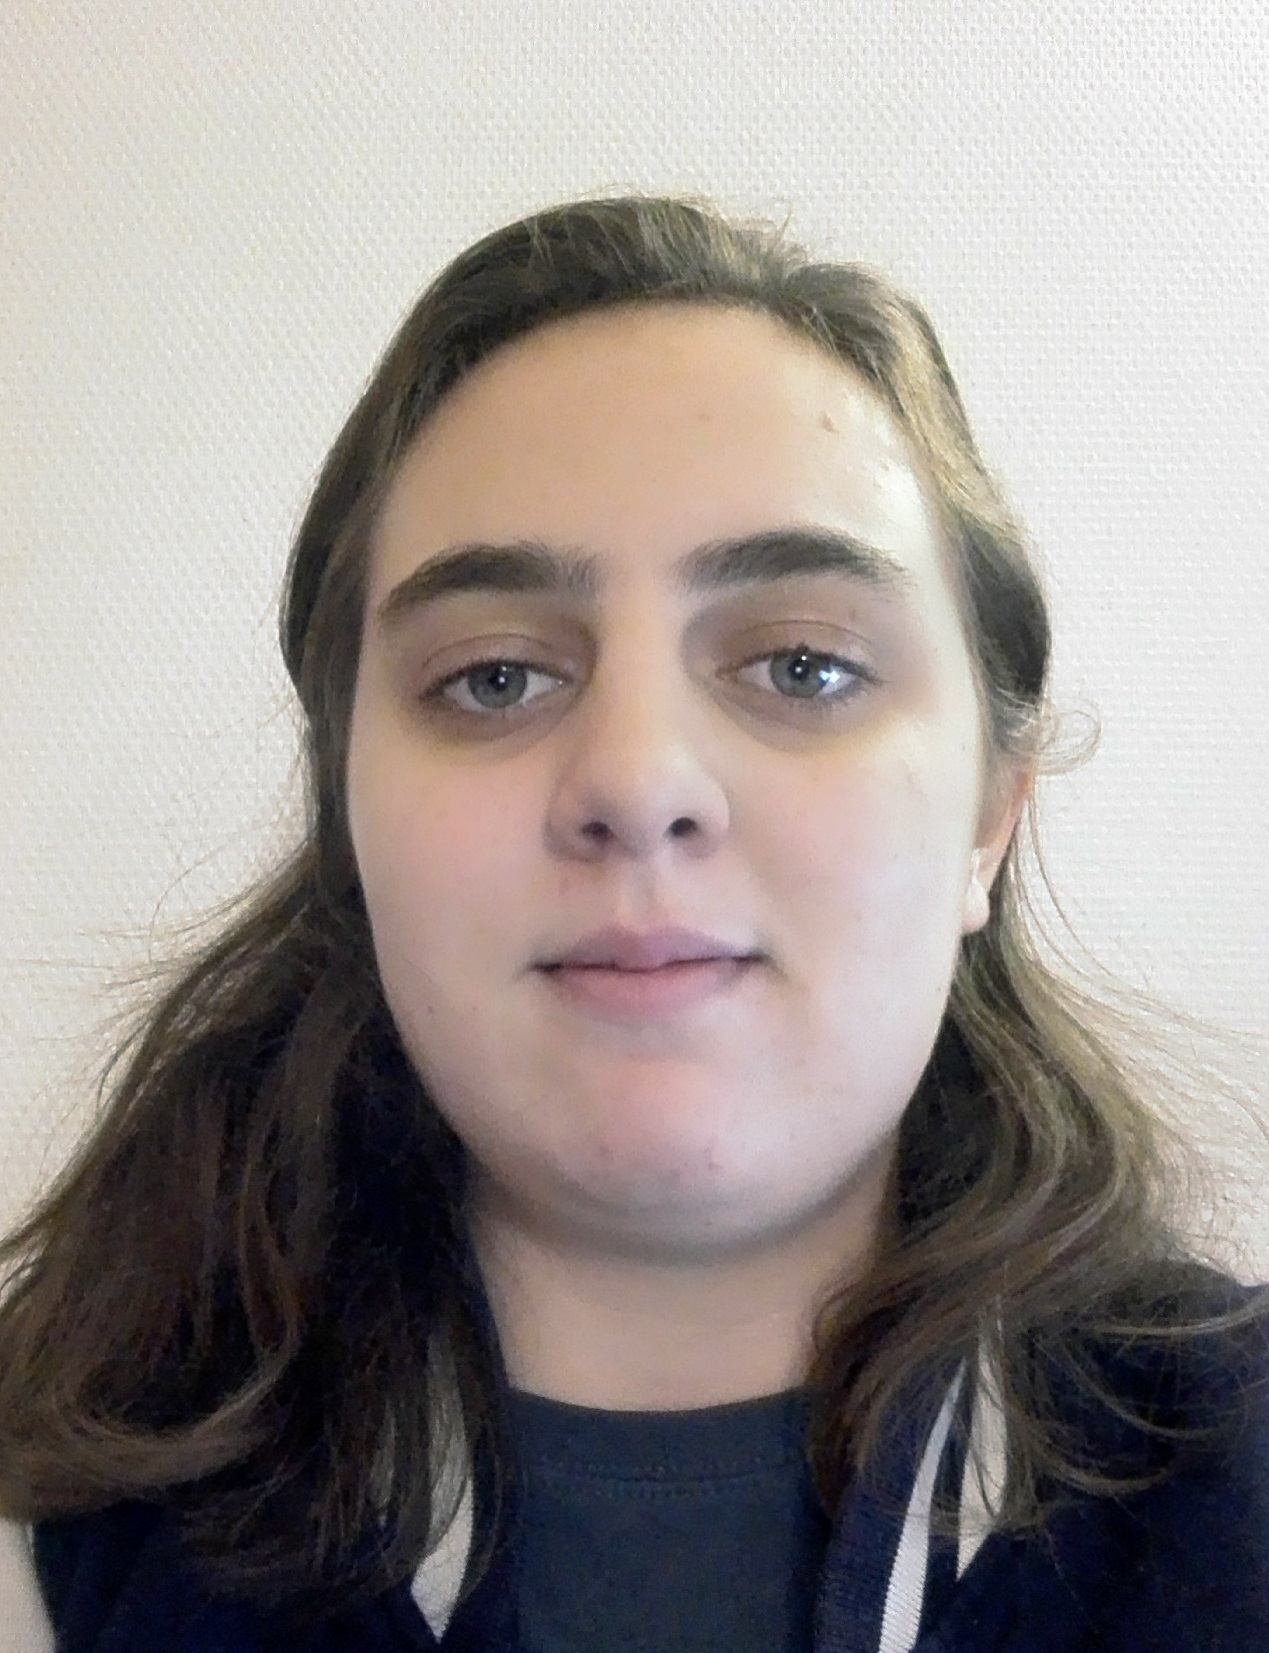
\includegraphics[height=4cm]{Annexes/Trombi_orgas/Tresorier}} & \multicolumn{3}{c|}{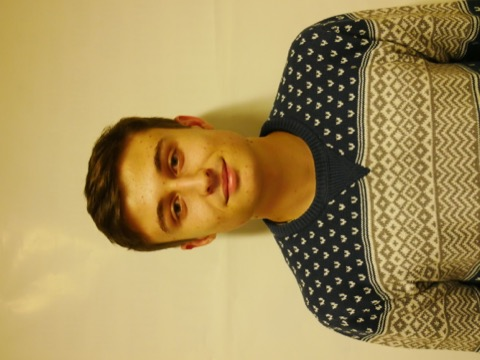
\includegraphics[height=4cm]{Annexes/Trombi_orgas/Orga_billetterie}} & \multicolumn{3}{c}{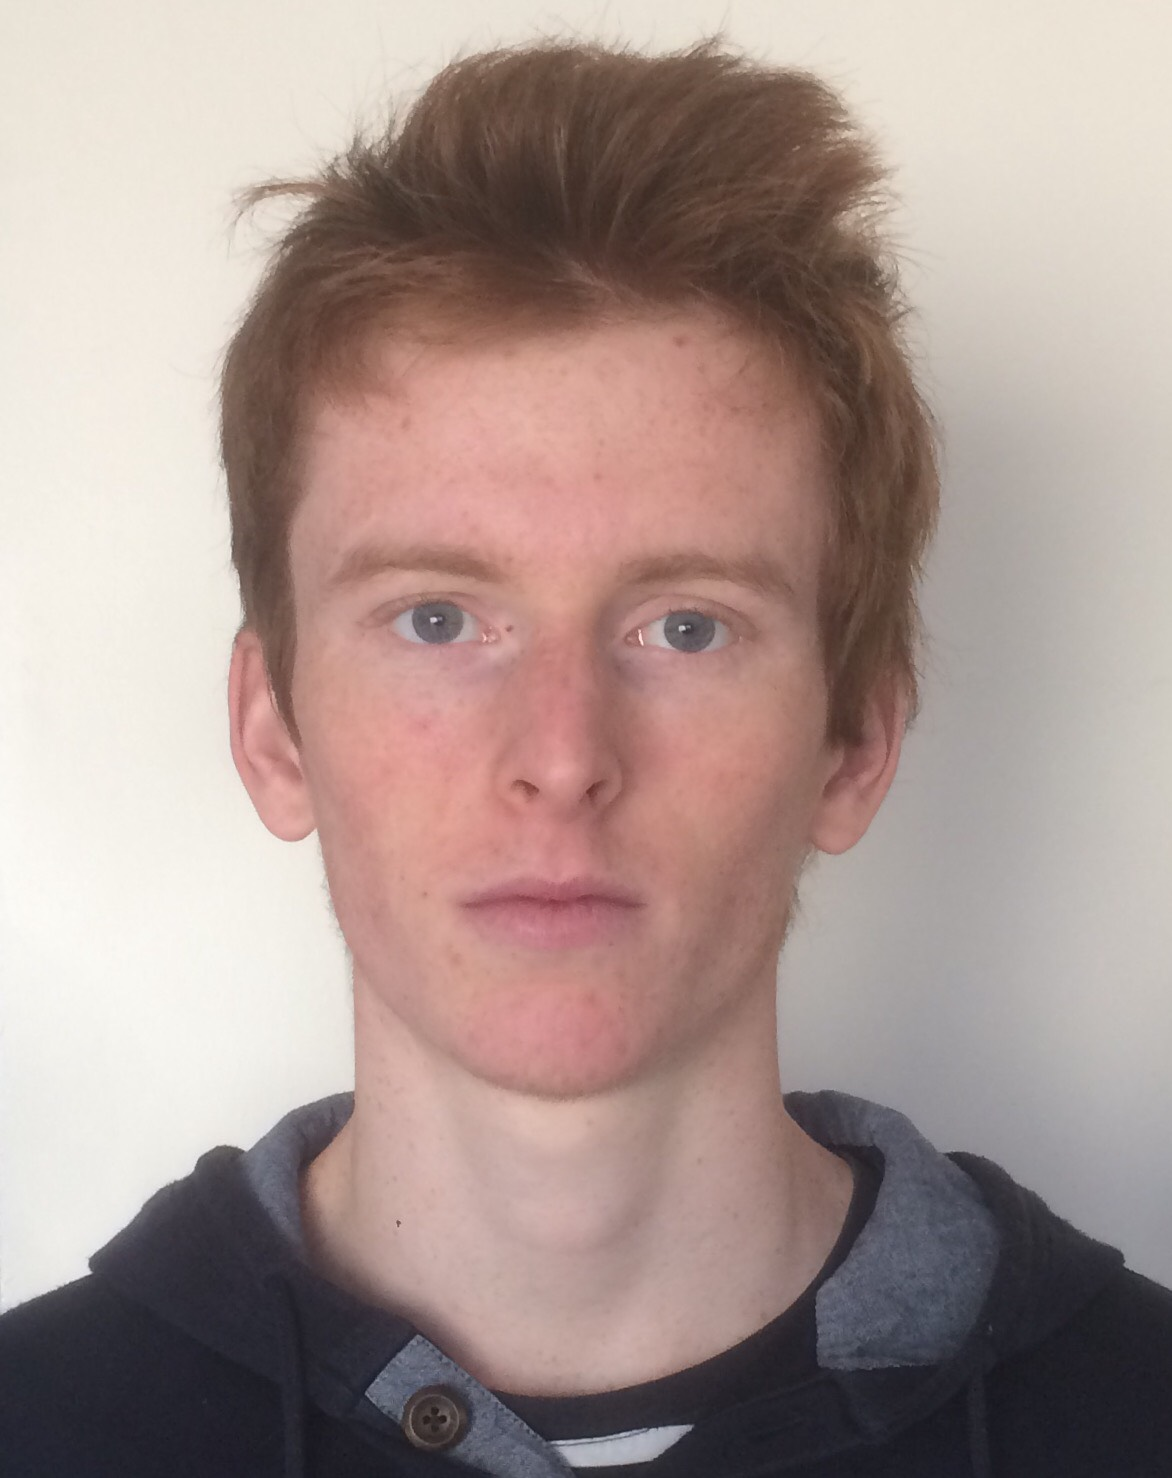
\includegraphics[height=4cm]{Annexes/Trombi_orgas/Orga_barriere_1}} & \multicolumn{3}{c|}{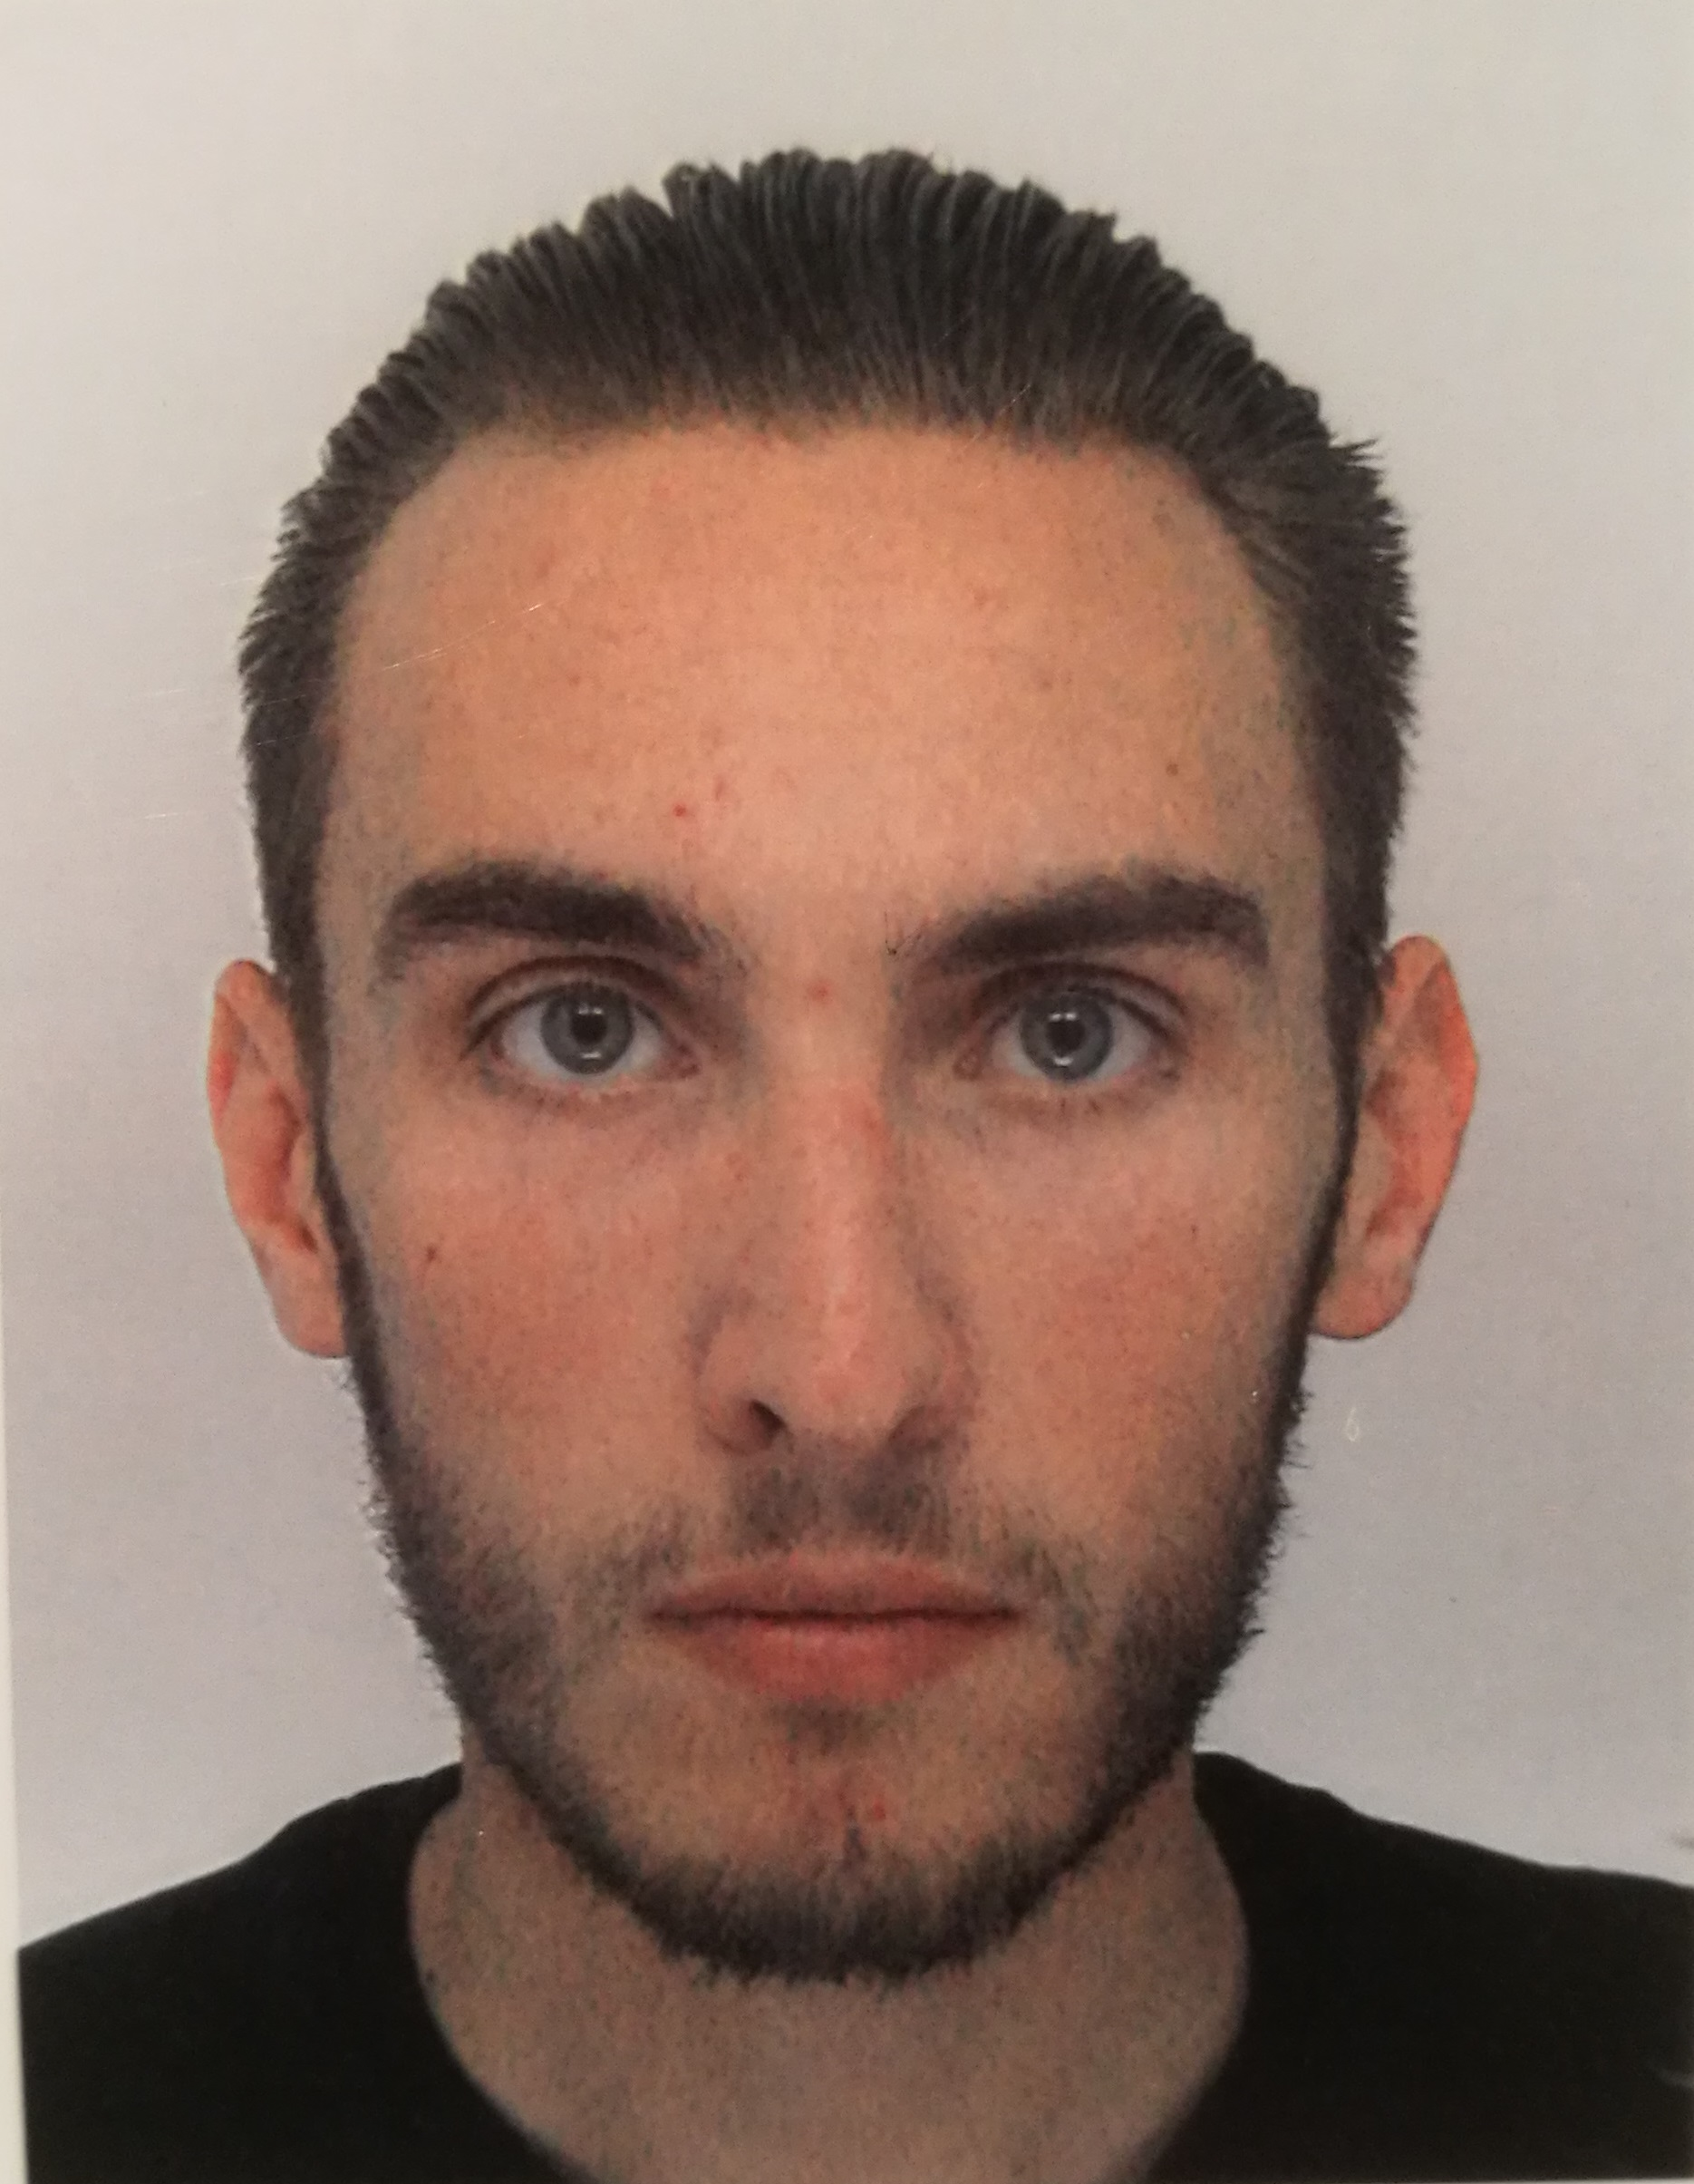
\includegraphics[height=4cm]{Annexes/Trombi_orgas/Orga_barriere_2}}\\
\multicolumn{3}{|c|}{Aline CLERC} & \multicolumn{3}{c|}{Hugo CANNEDDU} & \multicolumn{3}{c}{Adrian Damian} & \multicolumn{3}{c|}{Pierre-Yves TARDIEU}\\
\multicolumn{3}{|c|}{07 71 81 25 29} & \multicolumn{3}{c|}{06 80 99 47 91} & \multicolumn{3}{c}{06 44 05 66 98} & \multicolumn{3}{c|}{07 81 26 17 14}\\
\hline

\multicolumn{6}{|m{8cm}|}{} & \multicolumn{6}{m{8cm}|}{}\\
\multicolumn{6}{|c|}{\bf Responsables Bénévoles} & \multicolumn{6}{c|}{\bf Responsables Bars}\\
\multicolumn{6}{|c|}{orga@24heures.org} & \multicolumn{6}{c|}{restauration@24heures.org}\\
\multicolumn{3}{|c}{\rule{0pt}{2ex}} & \multicolumn{3}{c|}{} & \multicolumn{3}{c}{} & \multicolumn{3}{c|}{} \\
\multicolumn{3}{|c}{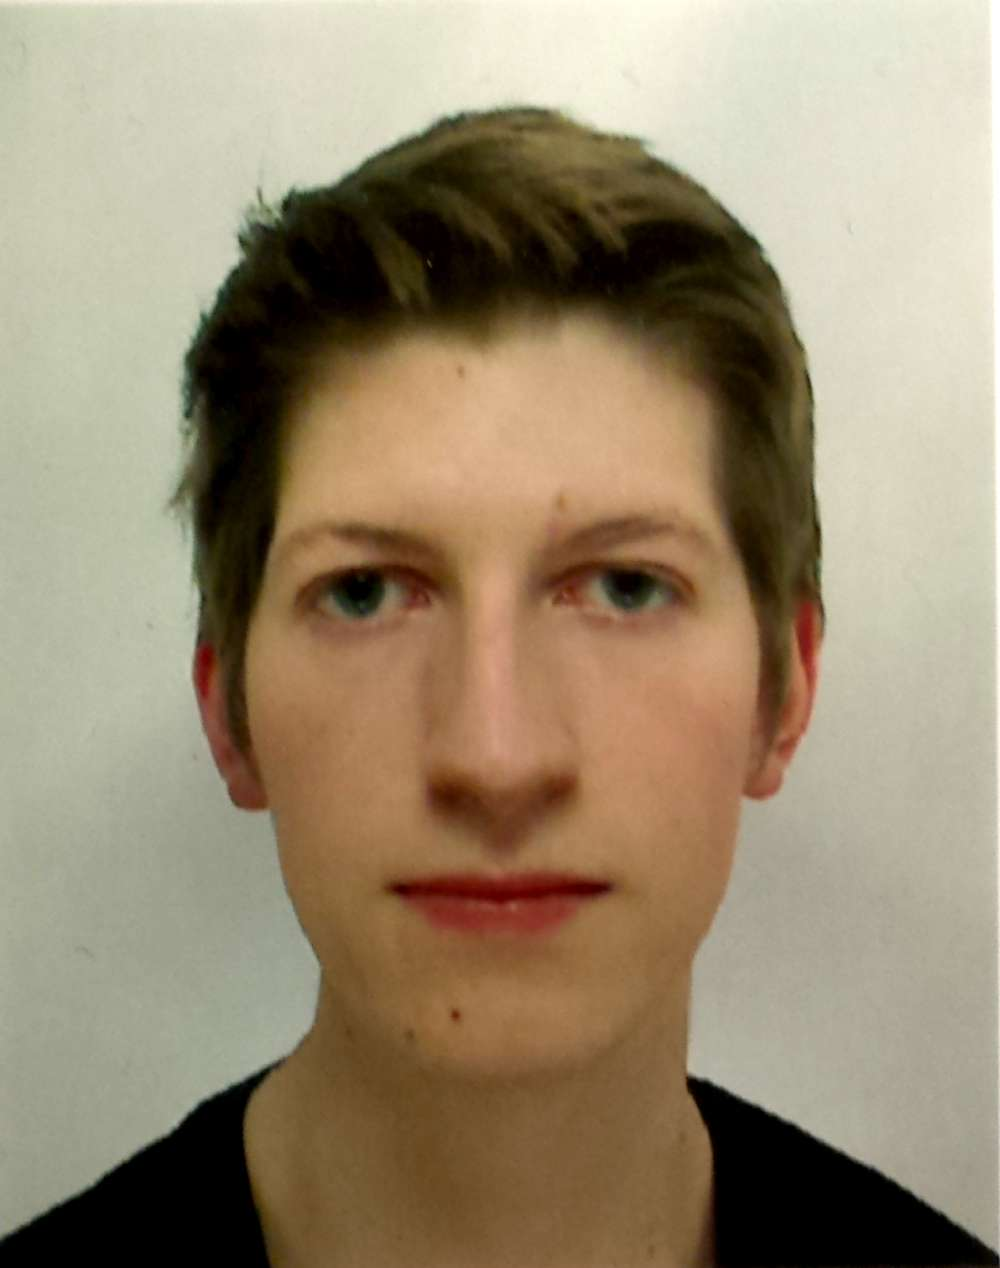
\includegraphics[height=4cm]{Annexes/Trombi_orgas/Orga_humain_1}} & \multicolumn{3}{c|}{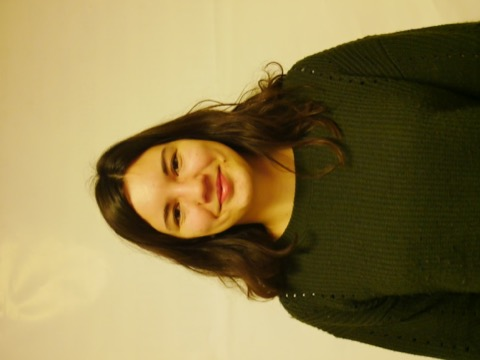
\includegraphics[height=4cm]{Annexes/Trombi_orgas/Orga_humain_2}} & \multicolumn{3}{c}{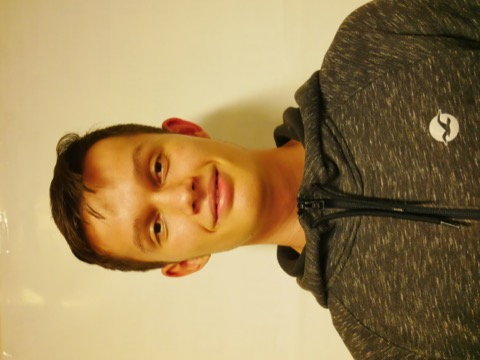
\includegraphics[height=4cm]{Annexes/Trombi_orgas/Orga_bar_1}} & \multicolumn{3}{c|}{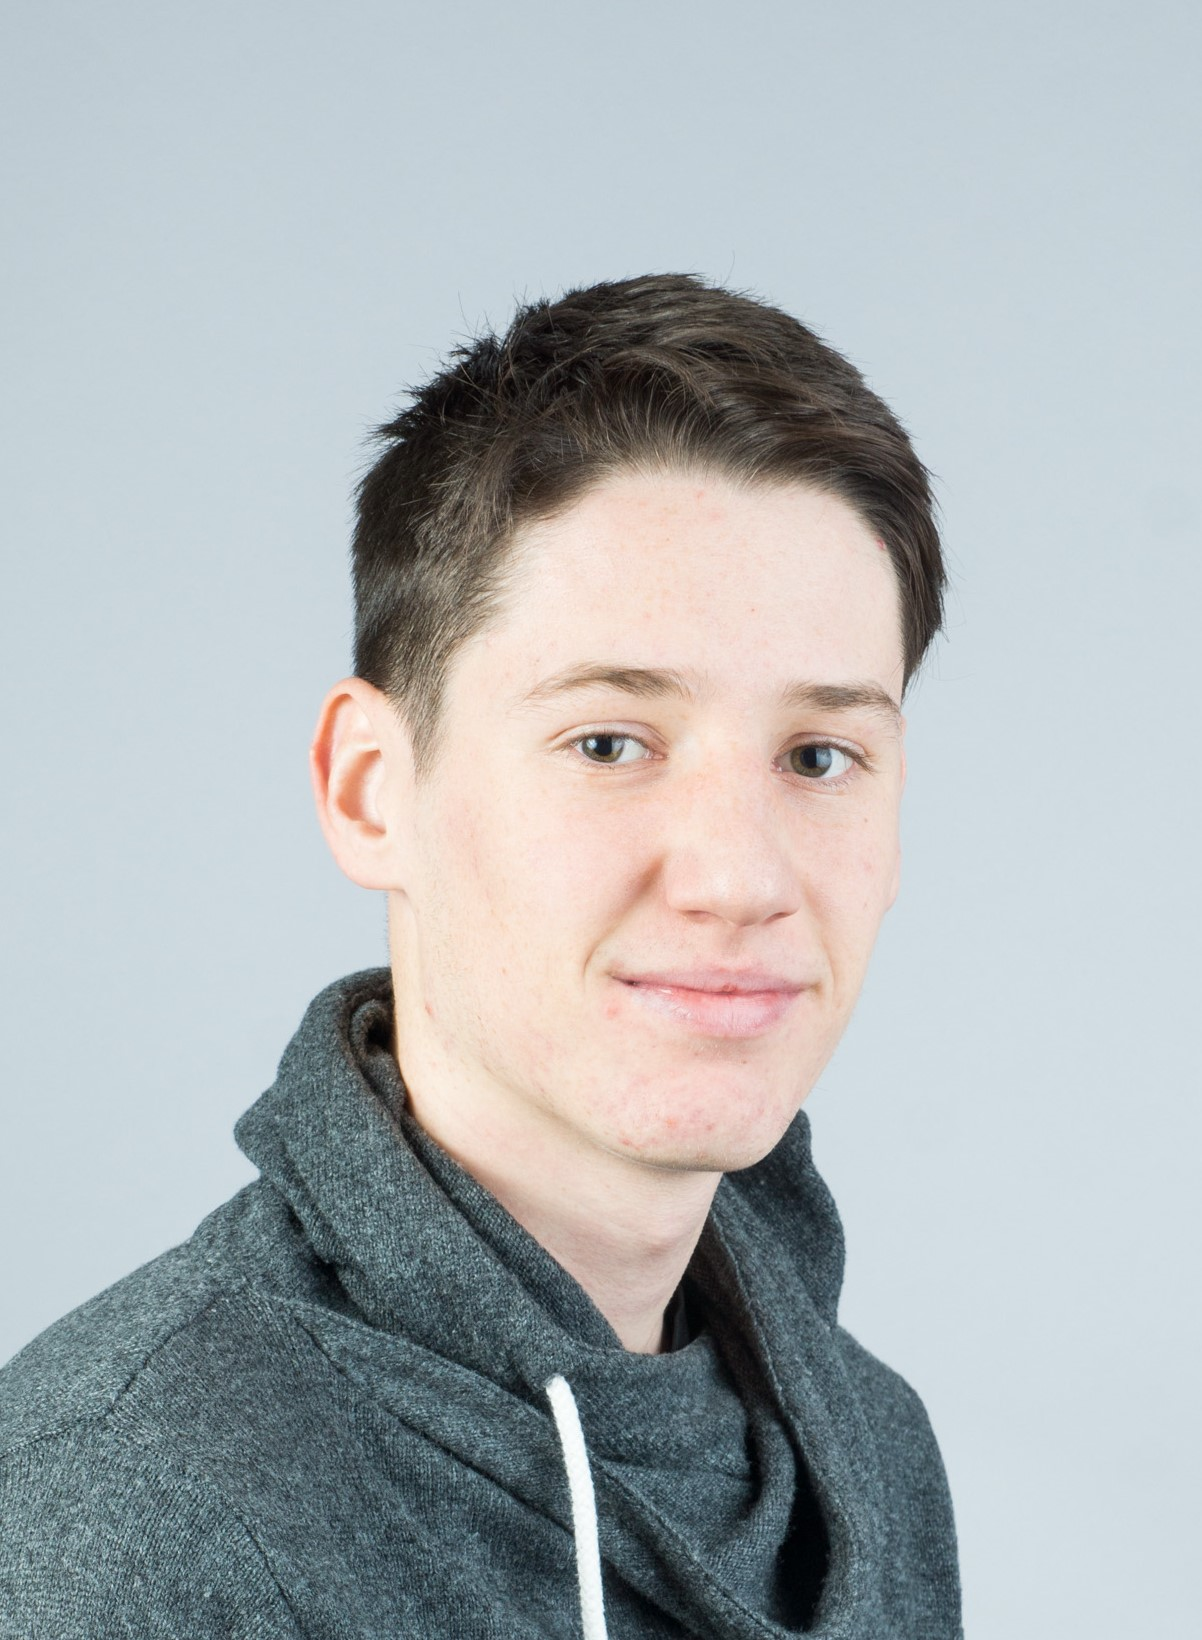
\includegraphics[height=4cm]{Annexes/Trombi_orgas/Orga_bar_2}}\\
\multicolumn{3}{|c}{Pedro GUEDES} & \multicolumn{3}{c|}{Elsa GASCON} & \multicolumn{3}{c}{Alexis LUZY} & \multicolumn{3}{c|}{Thomas GEORGES}\\
\multicolumn{3}{|c}{07 85 70 31 77} & \multicolumn{3}{c|}{06 88 13 16 72} & \multicolumn{3}{c}{07 61 09 64 48} & \multicolumn{3}{c|}{06 32 32 00 50}\\
\end{supertabular}

\newpage

\begin{supertabular}{|m{1.33cm}|m{1.33cm}|m{1.33cm}|m{1.33cm}|m{1.33cm}|m{1.33cm}|m{1.33cm}|m{1.33cm}|m{1.33cm}|m{1.33cm}|m{1.33cm}|m{1.33cm}|}
\shrinkheight{1cm}
\hline

\multicolumn{12}{|m{16cm}|}{}\\
\multicolumn{12}{|c|}{\bf Responsables Catering}\\
\multicolumn{12}{|c|}{catering24heures.org}\\
\multicolumn{4}{|m{5.33cm}}{\rule{0pt}{2ex}} & \multicolumn{4}{m{5.33cm}}{} & \multicolumn{4}{m{5.33cm}|}{} \\
\multicolumn{4}{|c}{\centering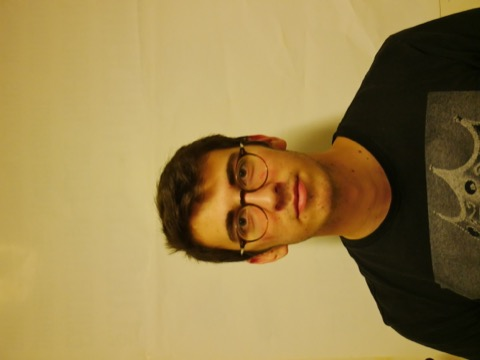
\includegraphics[height=4cm]{Annexes/Trombi_orgas/Orga_catering_1}}  & \multicolumn{4}{c}{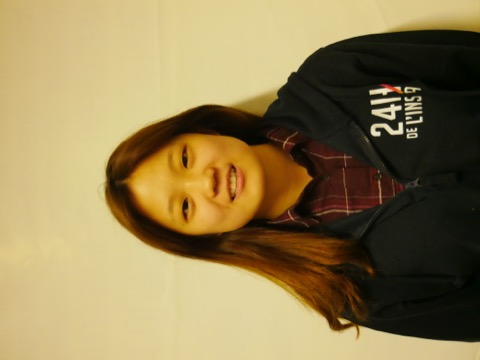
\includegraphics[height=4cm]{Annexes/Trombi_orgas/Orga_catering_2}} & \multicolumn{4}{c|}{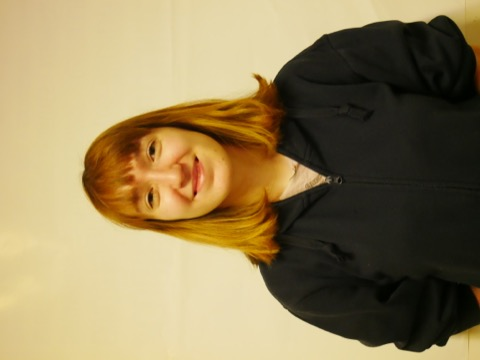
\includegraphics[height=4cm]{Annexes/Trombi_orgas/Orga_catering_3}} \\
\multicolumn{4}{|c}{Thibaut BELLANGER}  & \multicolumn{4}{c}{Han Yu} & \multicolumn{4}{c|}{Inès Garcia} \\
\multicolumn{4}{|c}{06 45 86 08 97}  & \multicolumn{4}{c}{07 83 22 58 61} & \multicolumn{4}{c|}{06 82 23 57 03} \\
\hline

\multicolumn{12}{|m{16cm}|}{}\\
\multicolumn{12}{|c|}{\bf Responsables Signalétique/Décoration}\\
\multicolumn{12}{|c|}{signaletique@24heures.org}\\
\multicolumn{4}{|m{5.33cm}}{\rule{0pt}{2ex}} & \multicolumn{4}{m{5.33cm}}{} & \multicolumn{4}{m{5.33cm}|}{} \\
\multicolumn{4}{|c}{\centering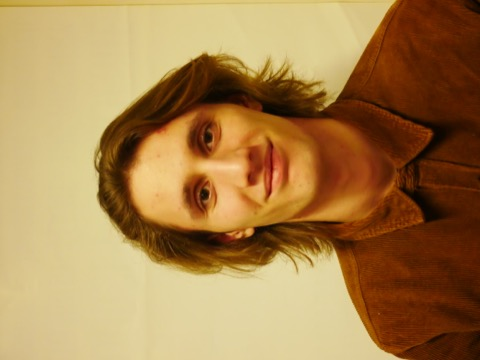
\includegraphics[height=4cm]{Annexes/Trombi_orgas/Orga_signa}}  & \multicolumn{4}{c}{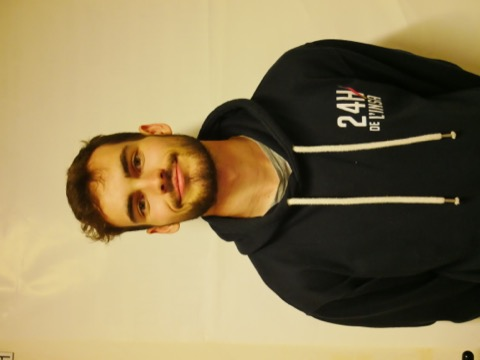
\includegraphics[height=4cm]{Annexes/Trombi_orgas/Orga_deco_1}} & \multicolumn{4}{c|}{
\includegraphics[height=4cm]{Annexes/Trombi_orgas/Orga_deco_2}} \\
\multicolumn{4}{|c}{Numa BAUBEAU}  & \multicolumn{4}{c}{Maxime CORNET} & \multicolumn{4}{c|}{Aude LECRIVAIN} \\
\multicolumn{4}{|c}{07 69 56 75 45}  & \multicolumn{4}{c}{06 99 11 69 37} & \multicolumn{4}{c|}{06 69 96 33 53} \\
\hline

\multicolumn{12}{|m{16cm}|}{}\\
\multicolumn{12}{|c|}{\bf Responsables Logistique}\\
\multicolumn{12}{|c|}{logistique@24heures.org}\\
\multicolumn{4}{|m{5.33cm}}{\rule{0pt}{2ex}} & \multicolumn{4}{m{5.33cm}}{} & \multicolumn{4}{m{5.33cm}|}{} \\
\multicolumn{4}{|c}{\centering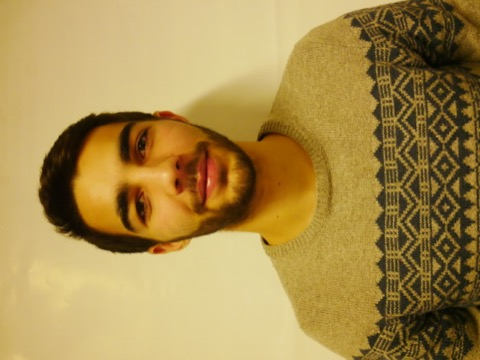
\includegraphics[height=4cm]{Annexes/Trombi_orgas/Orga_log_2}}  & \multicolumn{4}{c}{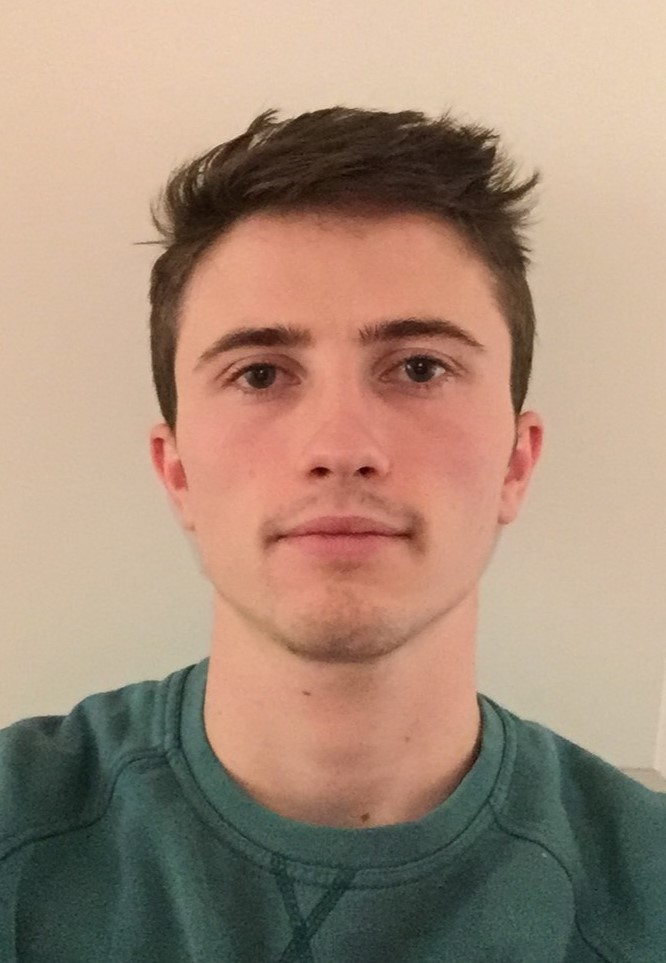
\includegraphics[height=4cm]{Annexes/Trombi_orgas/Orga_log_1}} & \multicolumn{4}{c|}{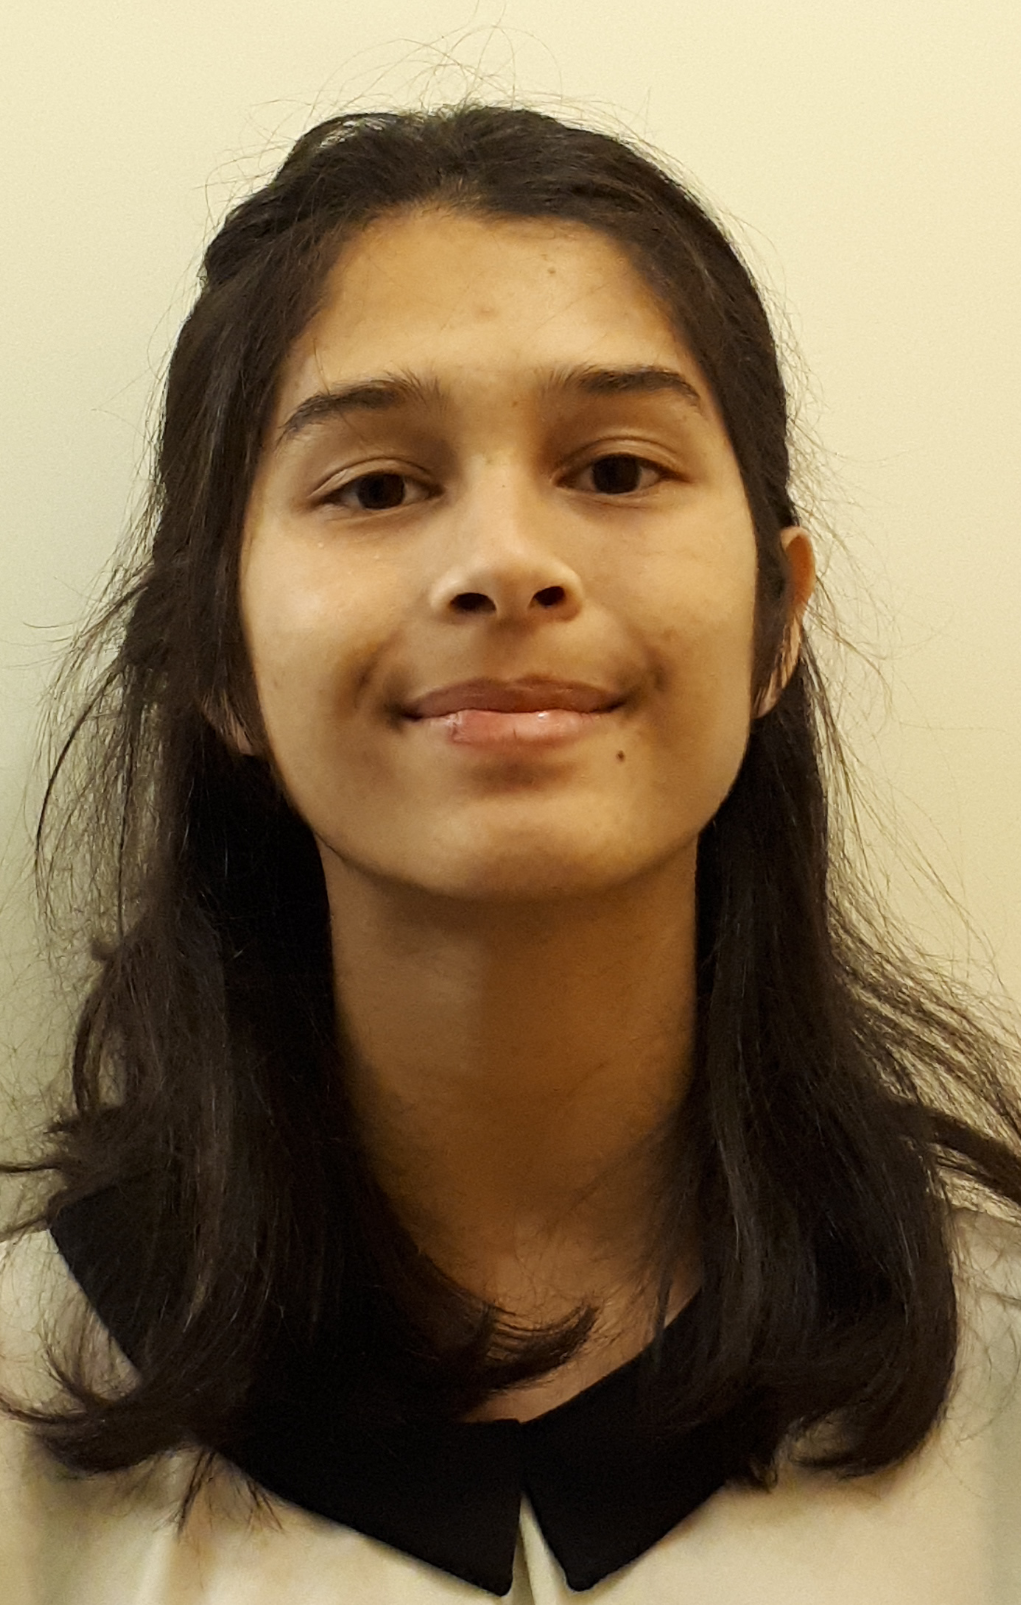
\includegraphics[height=4cm]{Annexes/Trombi_orgas/Orga_log_3}} \\
\multicolumn{4}{|c}{Louis-Pierre GAGNERE}  & \multicolumn{4}{c}{Majda QATIBI} & \multicolumn{4}{c|}{Nicolas GRELLIERE} \\
\multicolumn{4}{|c}{06 52 45 23 31}  & \multicolumn{4}{c}{06 63 54 30 06} & \multicolumn{4}{c|}{06 95 76 10 43} \\
\end{supertabular}

\newpage
\begin{supertabular}{|m{1.33cm}|m{1.33cm}|m{1.33cm}|m{1.33cm}|m{1.33cm}|m{1.33cm}|m{1.33cm}|m{1.33cm}|m{1.33cm}|m{1.33cm}|m{1.33cm}|m{1.33cm}|}
\shrinkheight{1cm}
\hline

\multicolumn{12}{|m{16cm}|}{}\\
\multicolumn{12}{|c|}{\bf Responsables Concerts}\\
\multicolumn{12}{|c|}{concerts@24heures.org}\\
\multicolumn{4}{|m{5.33cm}}{\rule{0pt}{2ex}} & \multicolumn{4}{m{5.33cm}}{} & \multicolumn{4}{m{5.33cm}|}{} \\
\multicolumn{4}{|c}{\centering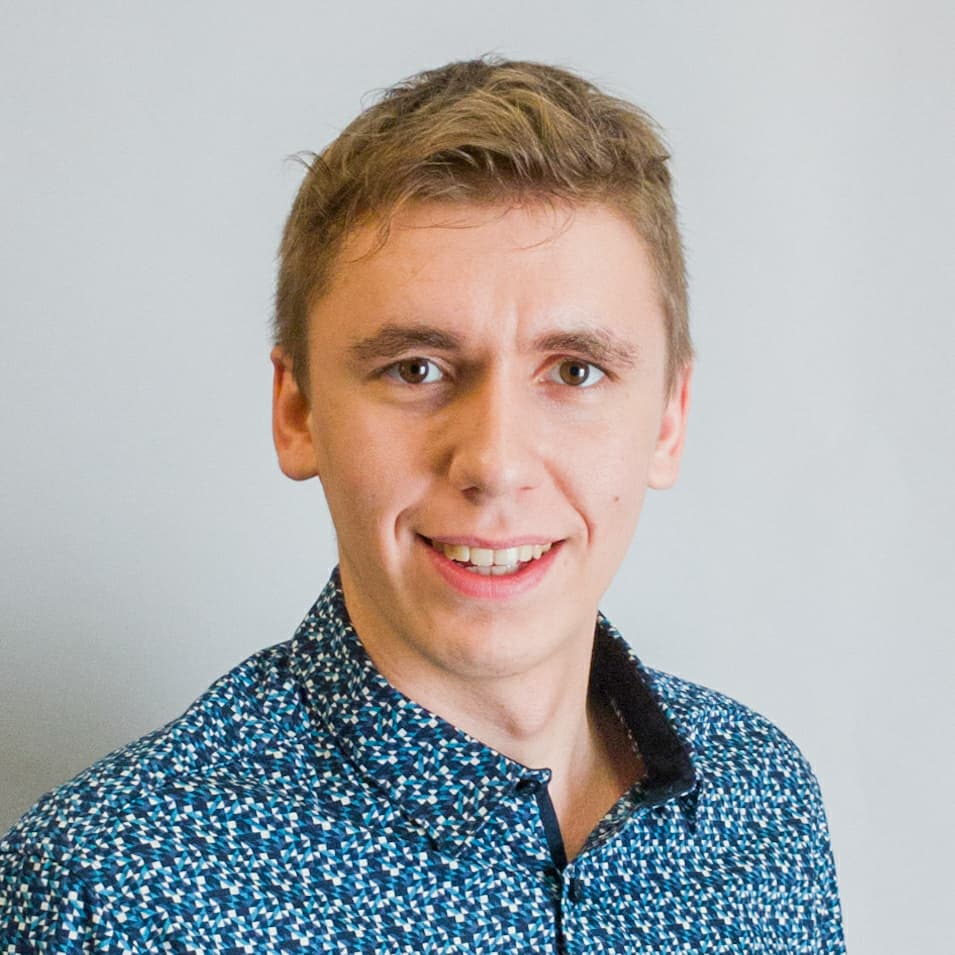
\includegraphics[height=4cm]{Annexes/Trombi_orgas/Orga_concert_1}}  & \multicolumn{4}{c}{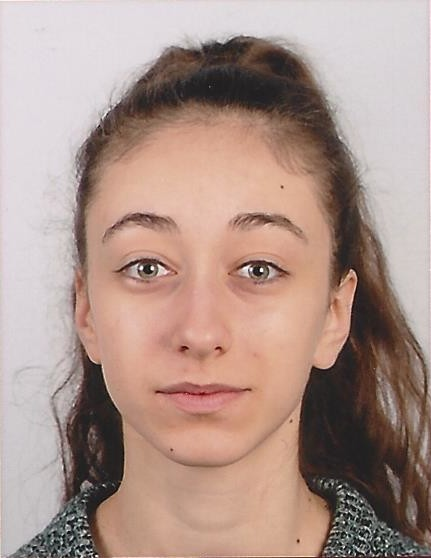
\includegraphics[height=4cm]{Annexes/Trombi_orgas/Orga_concert_2}} & \multicolumn{4}{c|}{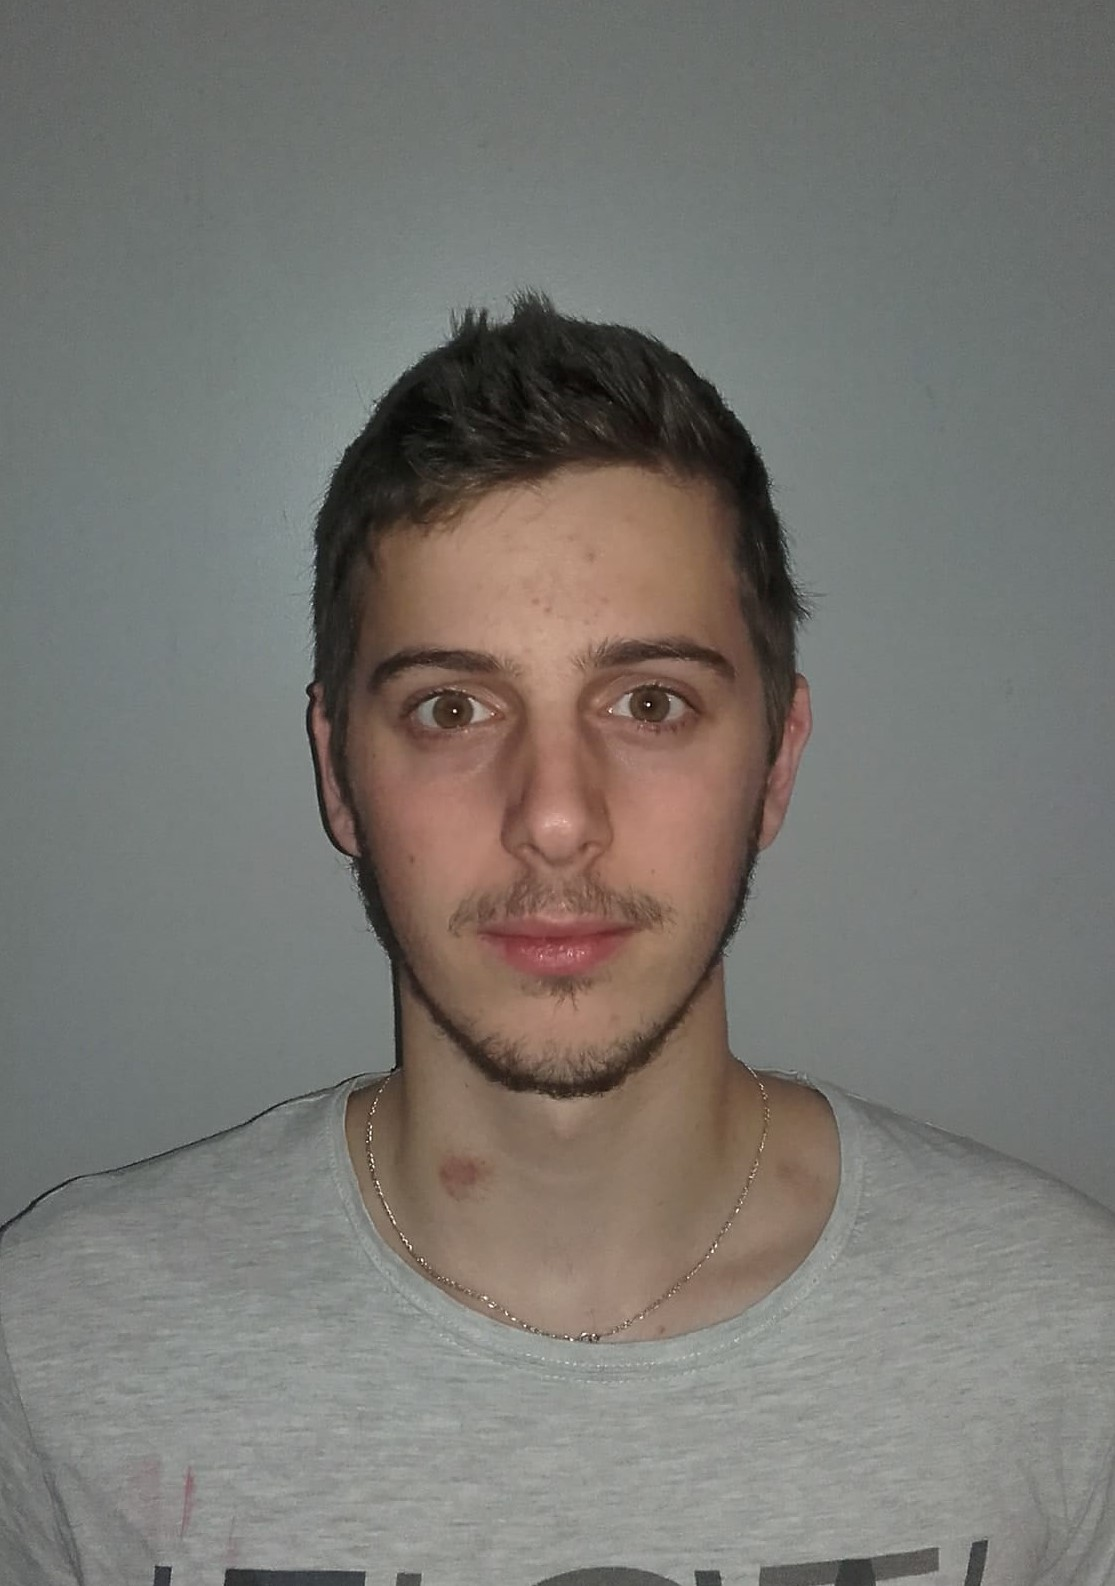
\includegraphics[height=4cm]{Annexes/Trombi_orgas/Orga_concert_3}} \\
\multicolumn{4}{|c}{Mathieu PORTELA}  & \multicolumn{4}{c}{Soline AUBERT} & \multicolumn{4}{c|}{Robin PLAGNES} \\
\multicolumn{4}{|c}{06 32 69 00 97}  & \multicolumn{4}{c}{06 96 28 76 23} & \multicolumn{4}{c|}{06 83 53 96 50} \\

\end{supertabular}

\tableofcontents
\label{table_matiere}
\newpage
\section{Préambule}

Ce dossier décrit les dispositions prévues à l’article 3 du Décret n°2002-887 du 3 mai 2002 pris pour l’application de l’article 23-1 de la loi n°95-73 du 21 janvier 1995 et relatif à certains rassemblements festifs à caractère musical, version consolidée au 30 juillet 2008.\\

Ce dossier s’appuie également sur les recommandations décrites dans la circulaire NOR/INT/E/88/00157/C du 20 avril 1988 relative à la sécurité des grands rassemblements. \\

Enfin, ce dossier décrit les mesures mises en place dans le cadre du plan Vigipirate.

\newpage

\section{Présentation de la manifestation}

Le festival des «24 heures de l’INSA» est une manifestation qui fêtera cette année sa 45\up{e}  édition. \\\\
En 1972 eut lieu ce qui devint par la suite l’événement fondateur des 24 heures : une course en vélo entre deux étudiants autour de deux bâtiments de l’INSA, pendant 24 heures. La course se reproduisit les années suivantes, s’entourant peu à peu d’animations diverses, jusqu'à devenir la manifestation d’aujourd'hui. Un week-end d’animations sportives, culturelles et ludiques, de défis sportifs (24h de course cycliste, 24h de course à pied, 24h de triathlon), et trois soirées de concerts, font désormais venir chaque année sur le même site plusieurs dizaines de milliers de personnes. Le public en journée est principalement constitué de familles et d’étudiants de la région lyonnaise. \\\\
En raison du nombre important de spectateurs qu’attirent les 24 heures de l'INSA, l'équipe organisatrice considère la sécurité comme sa priorité. L'essor de la manifestation et en particulier celui des concerts a conduit notre équipe à mieux communiquer avec tous les interlocuteurs de la protection des personnes et des biens.\\\\
Depuis 2006 la zone accueillant les concerts de la manifestation est considérée comme Établissement Recevant du Public. Conformément au règlement de sécurité du 25 juin 1980 modifié sur les dispositions générales, R 123.1 à 55 et R. 111.19 du ministère de l’intérieur et suivant le Code de la Construction et de l’habitation complété par l’arrêté du 6 janvier 1983 contre les risques d’incendie et de panique dans les établissements recevant du public, l’ensemble des dispositions spécifiques des établissements recevant du public de type plein air a été détaillé dans une notice ERP.\\\\
La manifestation organisée l’année dernière a été autorisée par la mairie de Villeurbanne, sur avis favorable de la Sous-commission Départementale de Sécurité ERP/IGH (Préfecture du Rhône) et la Sous-commission Départementale d’Accessibilité. Cette année encore nous nous appliquons à suivre ces réglementations.\\\\
L'objectif de ce dossier est de présenter dans le détail le dispositif de sécurité mis en place afin d'éviter les éventuels risques et le cas échéant minimiser leur impact possible. \\\\


\begin{minipage}[c]{.48\linewidth}
	  \begin{center}
      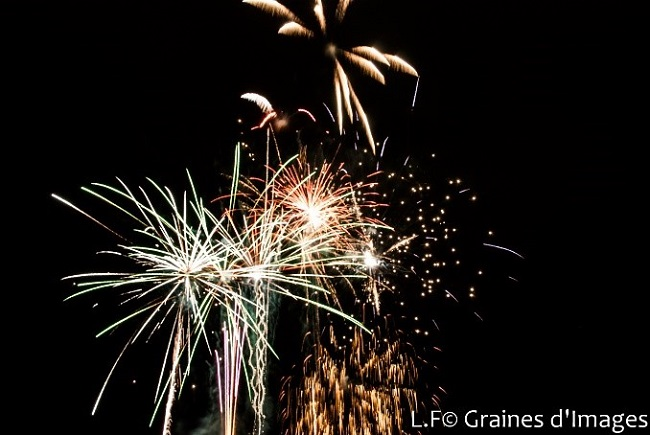
\includegraphics[scale =1]{Annexes/Images/prez1}
		\end{center}
 \end{minipage} \hfill
\begin{minipage}[c]{.48\linewidth}
		\begin{center}
      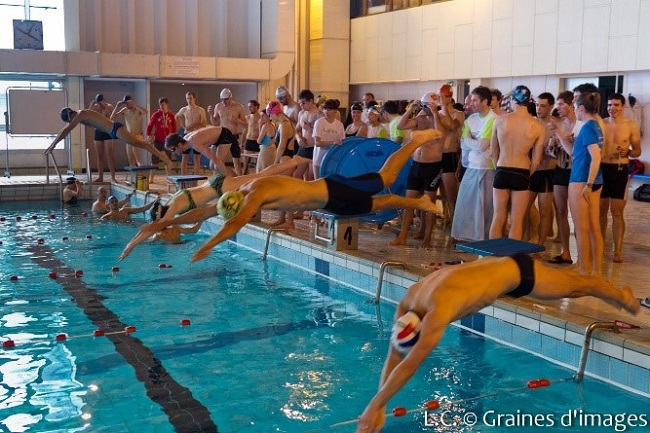
\includegraphics[scale =1]{Annexes/Images/prez2}
		\end{center}
\end{minipage}
\vspace{20mm}
\begin{minipage}[c]{.48\linewidth}
		\begin{center}
      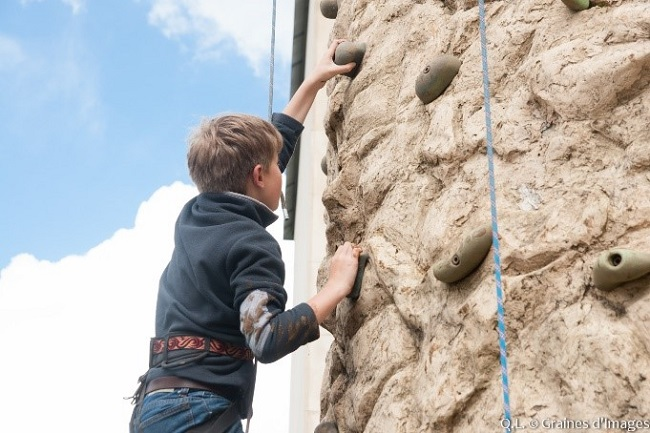
\includegraphics[scale =1]{Annexes/Images/prez3}
		\end{center}
\end{minipage} \hfill
\begin{minipage}[c]{.48\linewidth}
		\begin{center}
      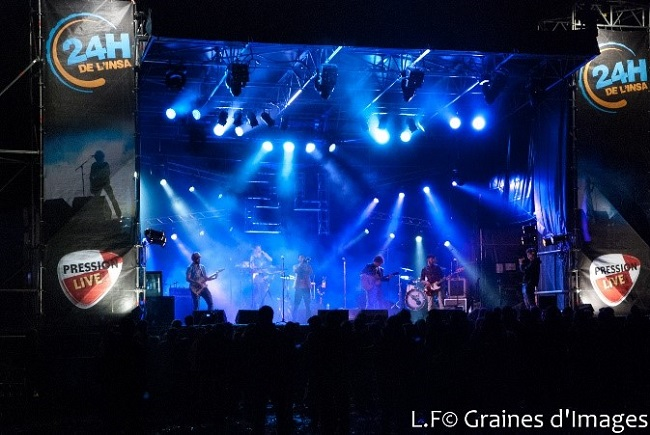
\includegraphics[scale =1]{Annexes/Images/prez4}
		\end{center}
\end{minipage}
\newpage
Le festival des 24 heures de l’INSA est organisé par une association loi 1901 qui porte le nom \textbf{Club des 24 heures de l’INSA.}
\begin{center}
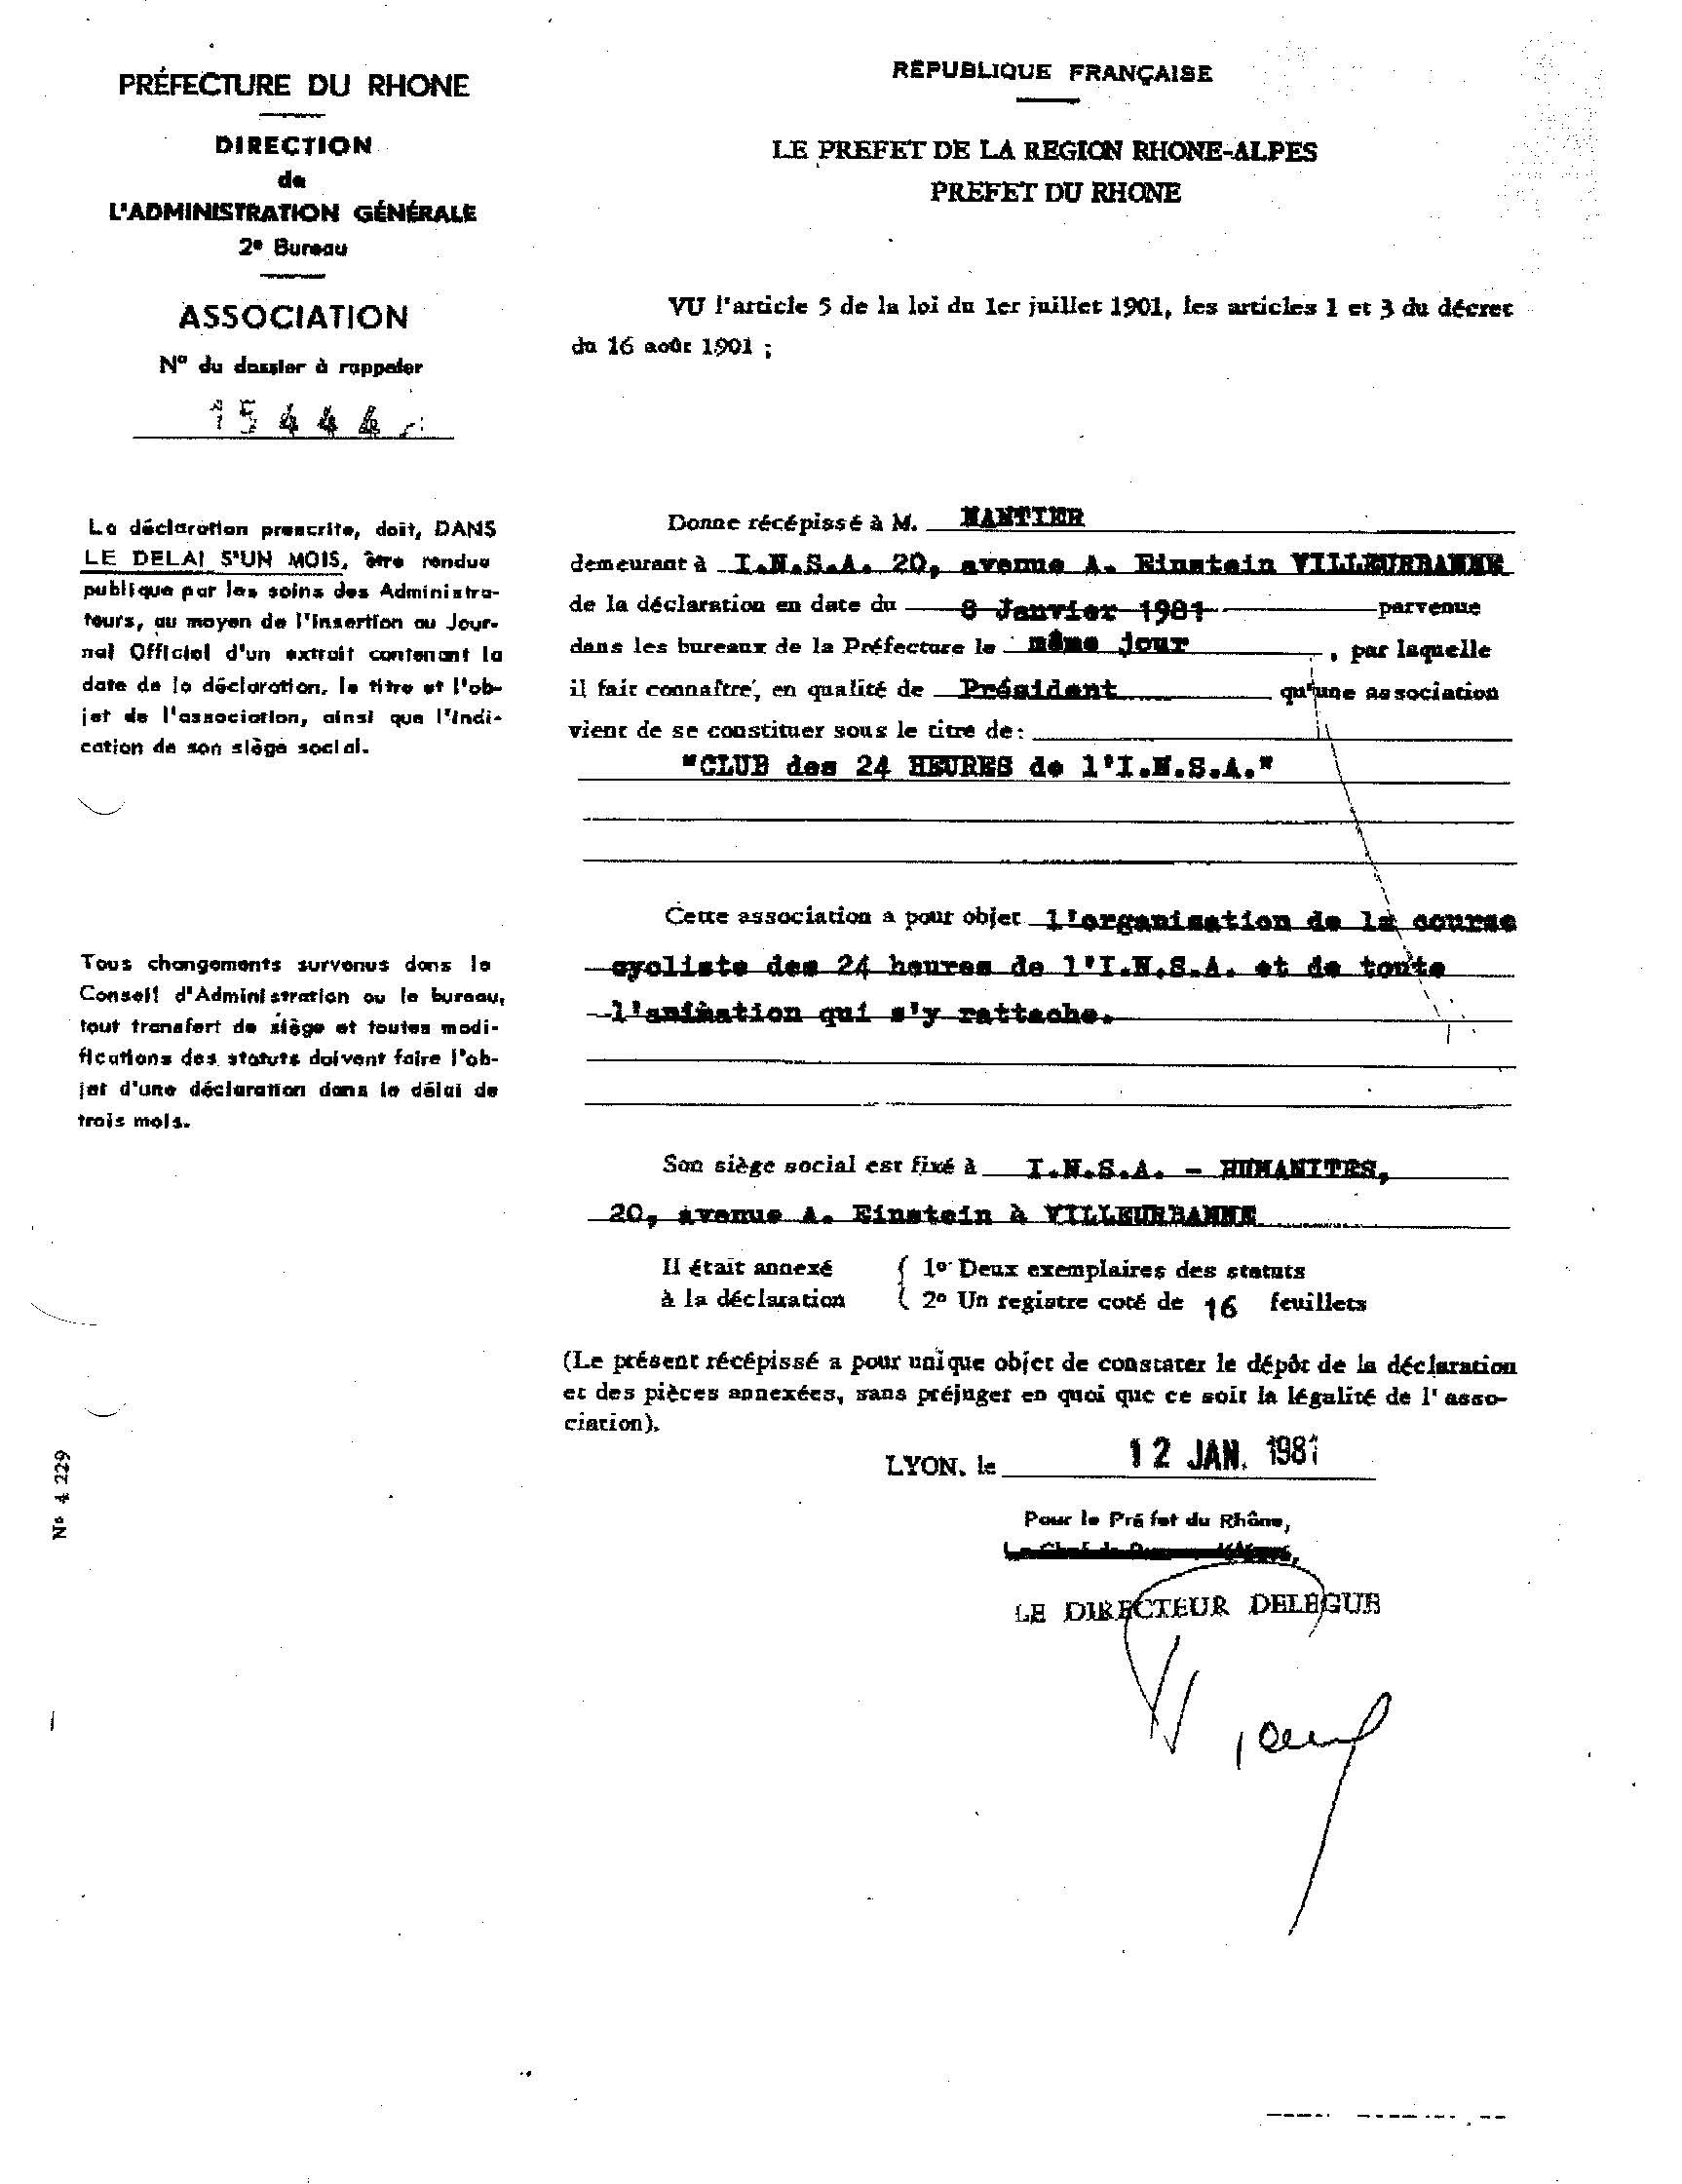
\includegraphics[scale=0.7]{Annexes/Images/decla}
\captionof{figure}{Récépissé de déclaration de l'association}
\end{center}

\newpage

\section{Résumé des modifications et nouveautés de l'édition 2019}

\setlength{\aboverulesep}{0pt}
\setlength{\belowrulesep}{0pt}
\setlength{\extrarowheight}{.75ex}
\begin{tabular}{|m{.15\textwidth}|m{.16\textwidth}|m{.47\textwidth}|m{.08\textwidth}|m{.04\textwidth}|} \toprule
\cellcolor[gray]{0.9} \centering\textbf{Chapitre concerné} & \cellcolor[gray]{0.9} \centering\textbf{Sous-partie} & \cellcolor[gray]{0.9} \centering\textbf{Modifications} & \cellcolor[gray]{0.9} \centering\textbf{Section}& \cellcolor[gray]{0.9} \textbf{Page}\\ \midrule
 & Calcul de l'effectif & Inchangé, la superficie de la zone est de 10 300 m\up{2}, soit 30 900 personnes. & \ref{calcul_de_leffectif}&\pageref{calcul_de_leffectif}\\
\cmidrule{2-5}
\vspace{1.5cm}
Sécurité incendie & Plan de l'ERP & 	Une zone de toilettes va être créée au nord du bâtiment Piscine, en plus de la zone de toilettes déjà existante au sud. 

Le chantier qui se situe au sud du bâtiment Coulomb devrait être terminé avant la manifestation, et si ce n'est pas le cas la zone de chantier sera dégagée et le barriérage reprendra exactement le même tracé, afin de ne pas modifier la taille de la zone. Les travaux au nord de Jacquard débuteront après la fin de la manifestation.& \ref{refPlanERP}&\pageref{refPlanERP}\\
\cmidrule{2-5}
& Espace VIP & Un espace VIP a été aménagé au nord du batiment Jaquard. & \ref{espace_VIP}&\pageref{espace_VIP}\\
\cmidrule{2-5}
& Infrastructures scéniques & Nous changeons de prestataire et donc d'infrastructure scénique. La résistance au vent de la Grande Scène est accrue. & \ref{Grande_scene}&\pageref{Grande_scene}\\
\midrule
\vspace{1.8cm}
Sûreté et Risques & Emplacement du PCS et du PCO & Nous avons mutualisé les emplacements du PCS et du PCO pour simplifier nos procédures d'armement de ce dernier. Afin d'avoir suffisamment d'espace pour tout le matériel nécessaire, nous utiliserons dorénavant une salle au 2\up{ème} étage de la Bibliothèque Marie Curie. & \ref{coordination_effectifs}

\ref{refProcedurePMA}&\pageref{coordination_effectifs}

\pageref{refProcedurePMA}\\
\cmidrule{2-5}
 & Dispositif anti-bélier & Création d'un deuxième périmètre de bloquage de circulation autour de la zone de plus forte affluence (la zone des entrées). & \ref{perimetre}&\pageref{perimetre}\\
\cmidrule{2-5}
 & Gestion des déchets & Ajout de poubelles de type "sac à gravats" & \ref{gestion_dechets} & \pageref{gestion_dechets}\\
\midrule
Plan Vigipirate & Nouvelles directives & Prise en compte des nouvelles directives parues depuis l'édition 2018. & \ref{refVigipirate}&\pageref{refVigipirate}\\
\midrule
\vspace{1.8cm}
Nouvelles animations & Kart à pédales & Un circuit de karts à pédales sera installé sur les terrains de tennis. Les bordures de pistes seront matérialisées par des structures gonflables. & \ref{kart_à_pédales}&\pageref{kart_à_pédales}\\
\cmidrule{2-5}
 & Mur des champions & Il s'agit d'une structure inclinée de 7 mètres de haut sur laquelle les participants se hissent à la force de leurs bras. & \ref{mur_des_champions} & \pageref{mur_des_champions}\\
\cmidrule{2-5}
 & Bobine Tesla & Une bobine tesla qui produits des éclairs sera installées sur le terrain stabilisé au nord de la piscine avant le feu d'artifice. Des dispositifs de sécurité sont mis en place à ce sujet. & \ref{bobine_tesla} & \pageref{bobine_tesla}\\
\midrule
Accessibilité & Cabinet d'aisance & L'emplacement du cabinet d'aisance pour les PMR à été modifié. & \ref{toilette_PMR}&\pageref{toilette_PMR}\\
\bottomrule

\end{tabular}

\newpage

%------------------------------------------------------------------------------------------------------
%SECURITE INCENDIE
%------------------------------------------------------------------------------------------------------

\chapter{ Sécurité Incendie}

\section{Plan de masse}

\begin{center}
	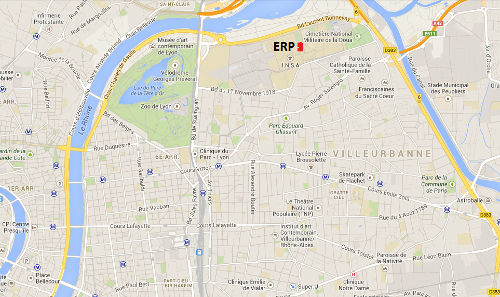
\includegraphics[width=.8\textwidth,keepaspectratio]{Annexes/Images/plandemasse}
	\captionof{figure}{Plan de Villeurbanne et situation de l’ERP}
	\vspace{5mm}
	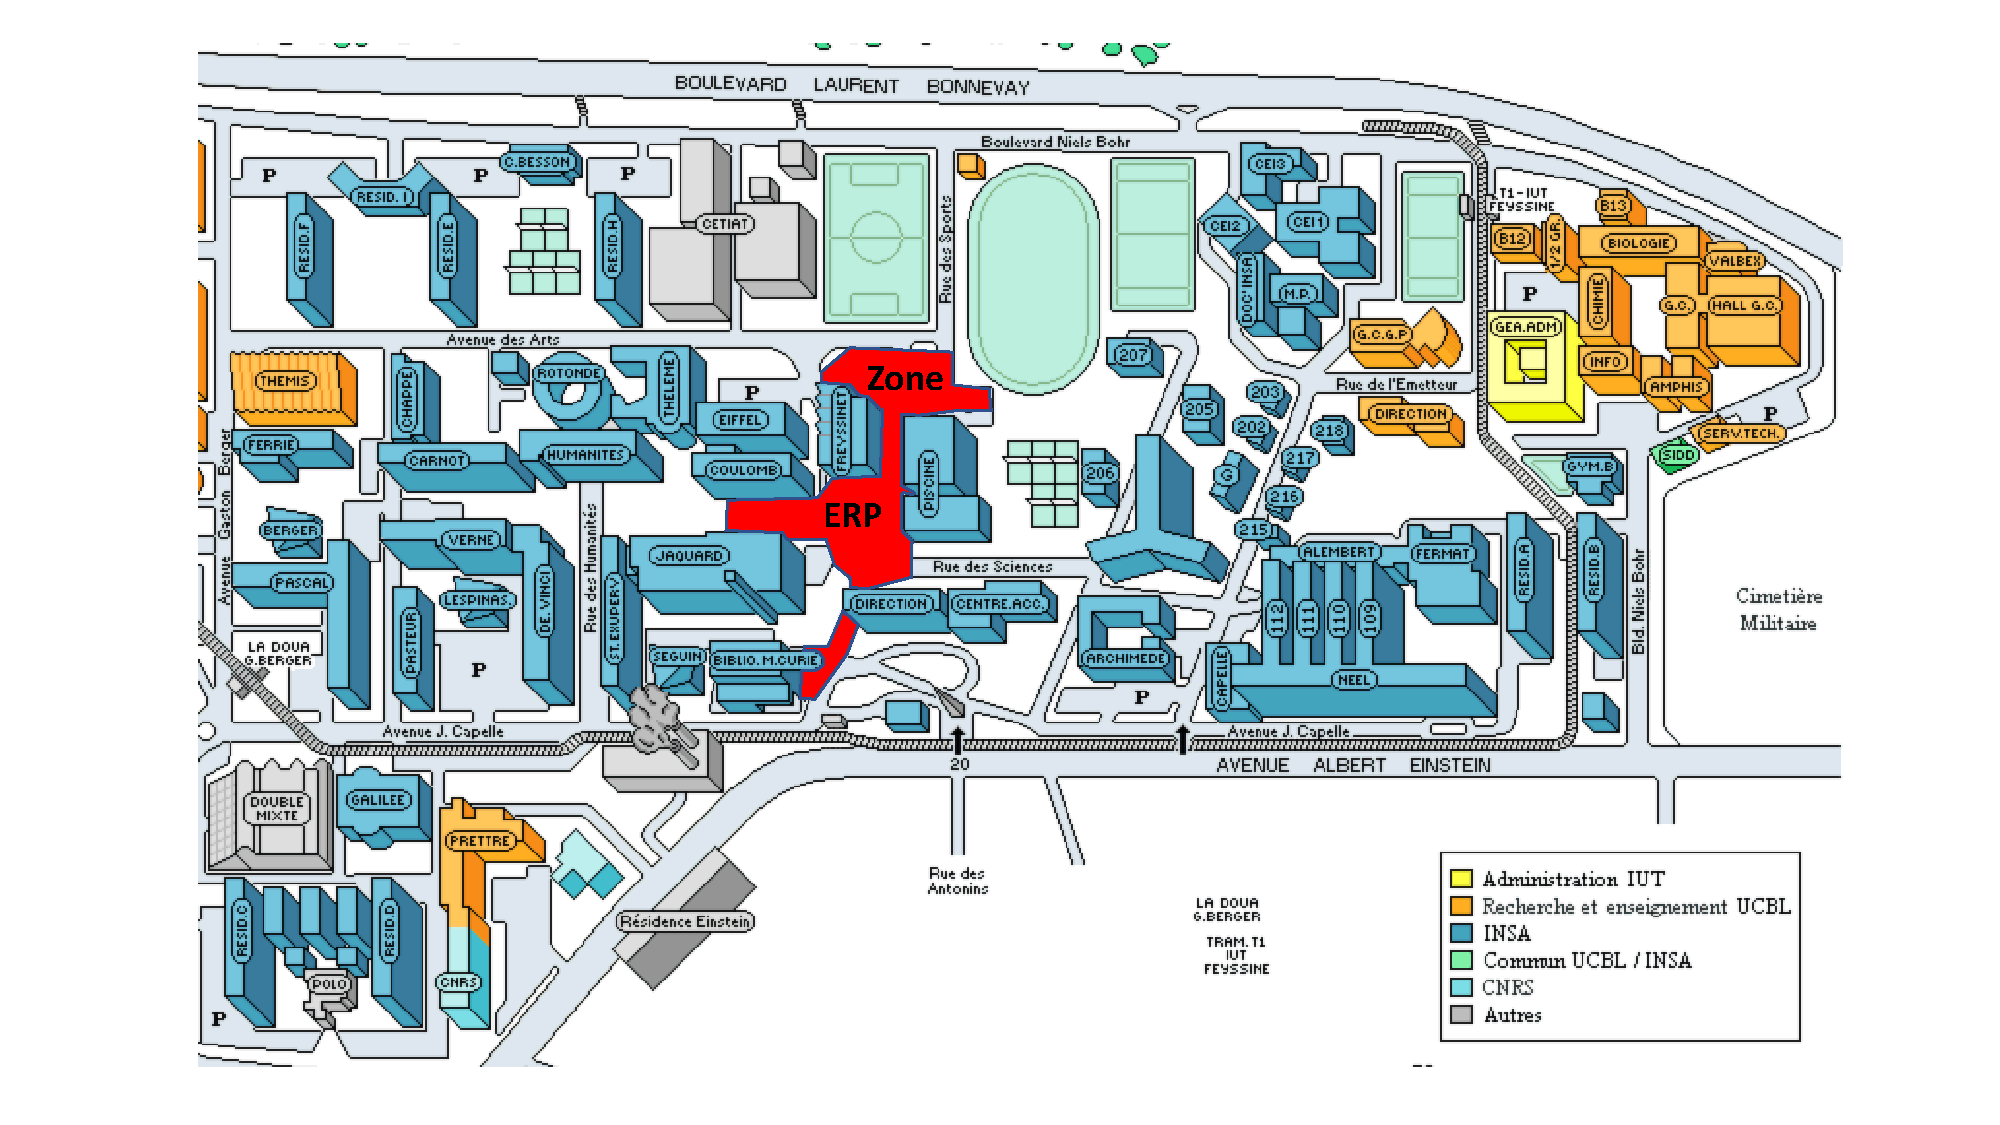
\includegraphics[width=\textwidth,keepaspectratio, angle=90]{Annexes/Exports/Plan_du_campus}
	\captionof{figure}{Plan du Campus de la Doua - LyonTech et situation de l'ERP}
\end{center}

\section{Plan de situation}

\begin{center}
	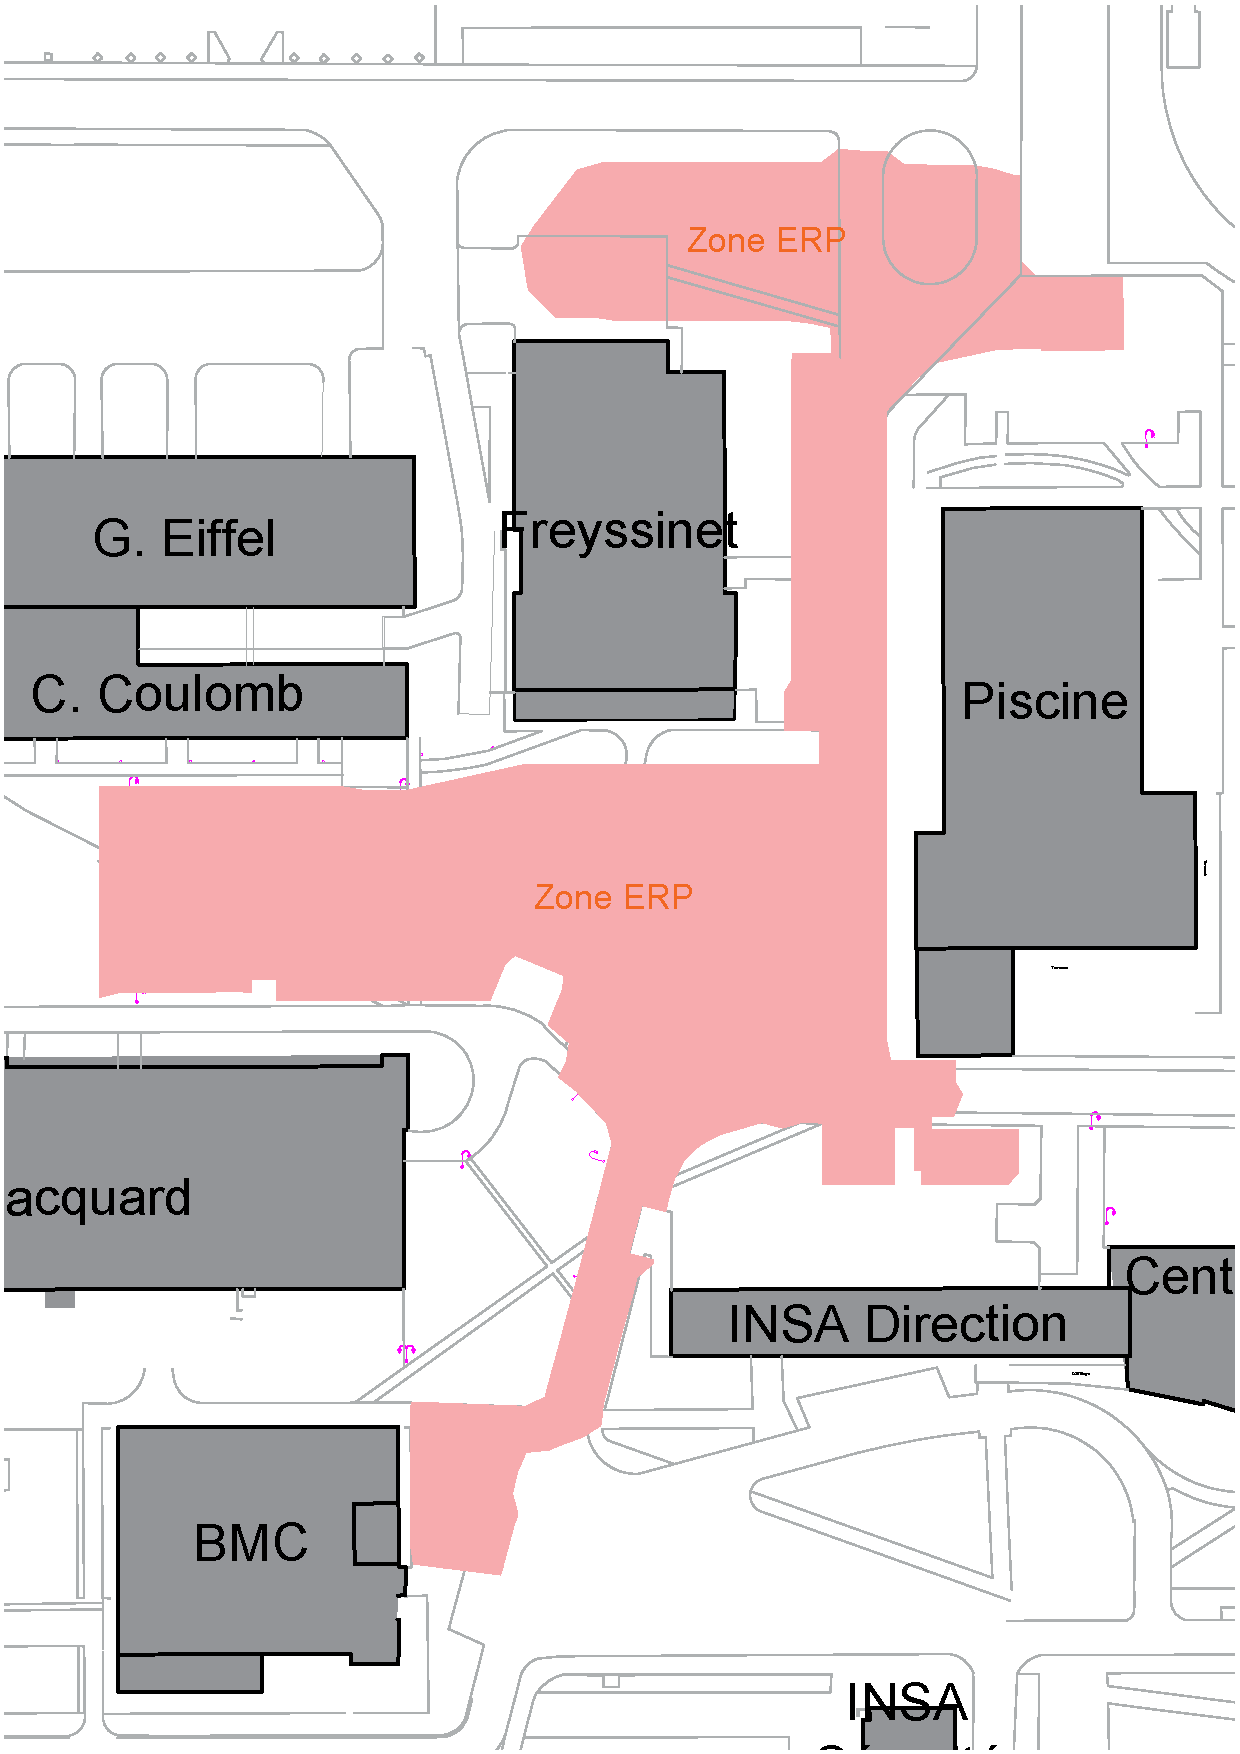
\includegraphics[width=.8\textwidth,keepaspectratio]{Exports/Plan_24h_44eme-Plan_de_situation}
	\captionof{figure}{Plan de la zone ERP et des alentours}
	\vspace{5mm}
	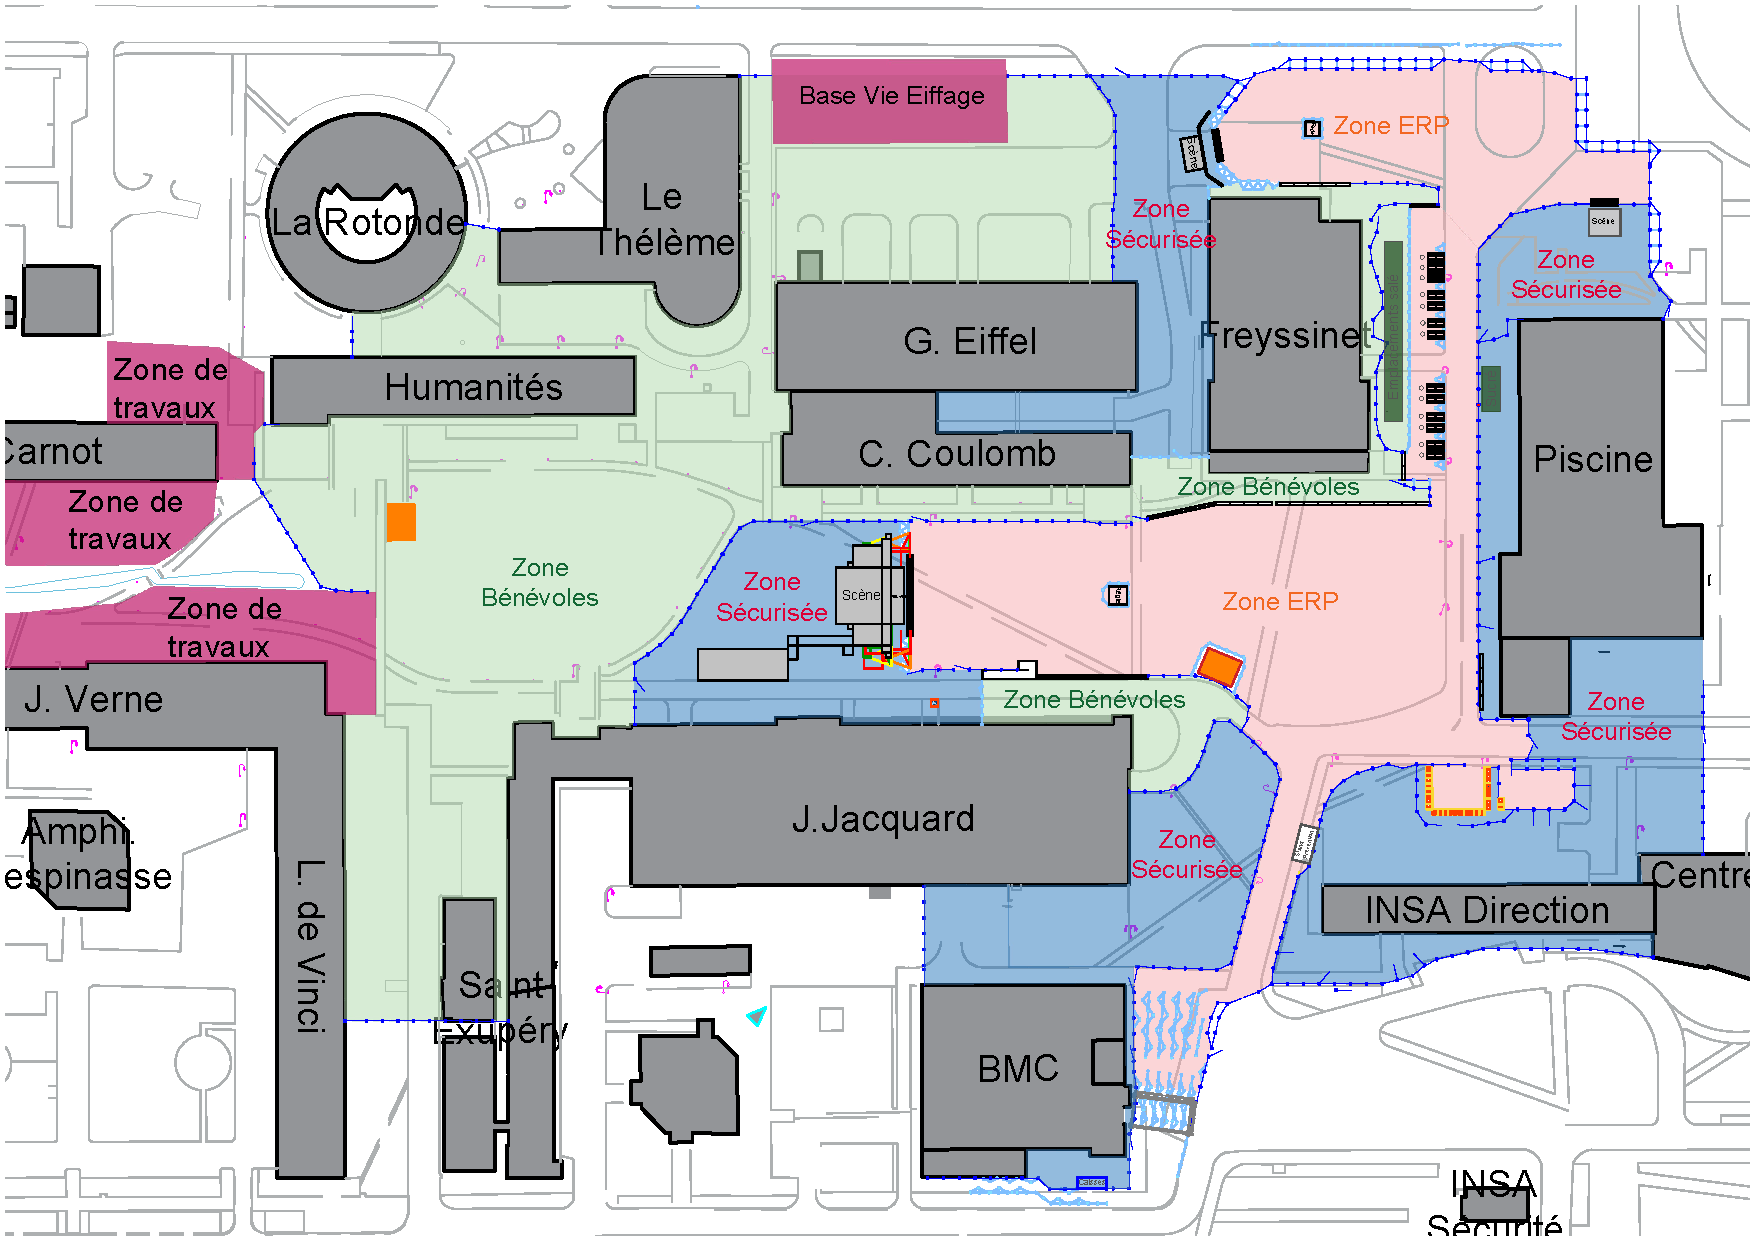
\includegraphics[angle=90,scale=0.7]{Exports/Plan_24h_44eme-Plan_ERP}
	\captionof{figure}{\label{refPlanERP}Plan de l'ERP édition 2018}
\end{center}

\section{Vue aérienne de la zone}

\begin{center}
	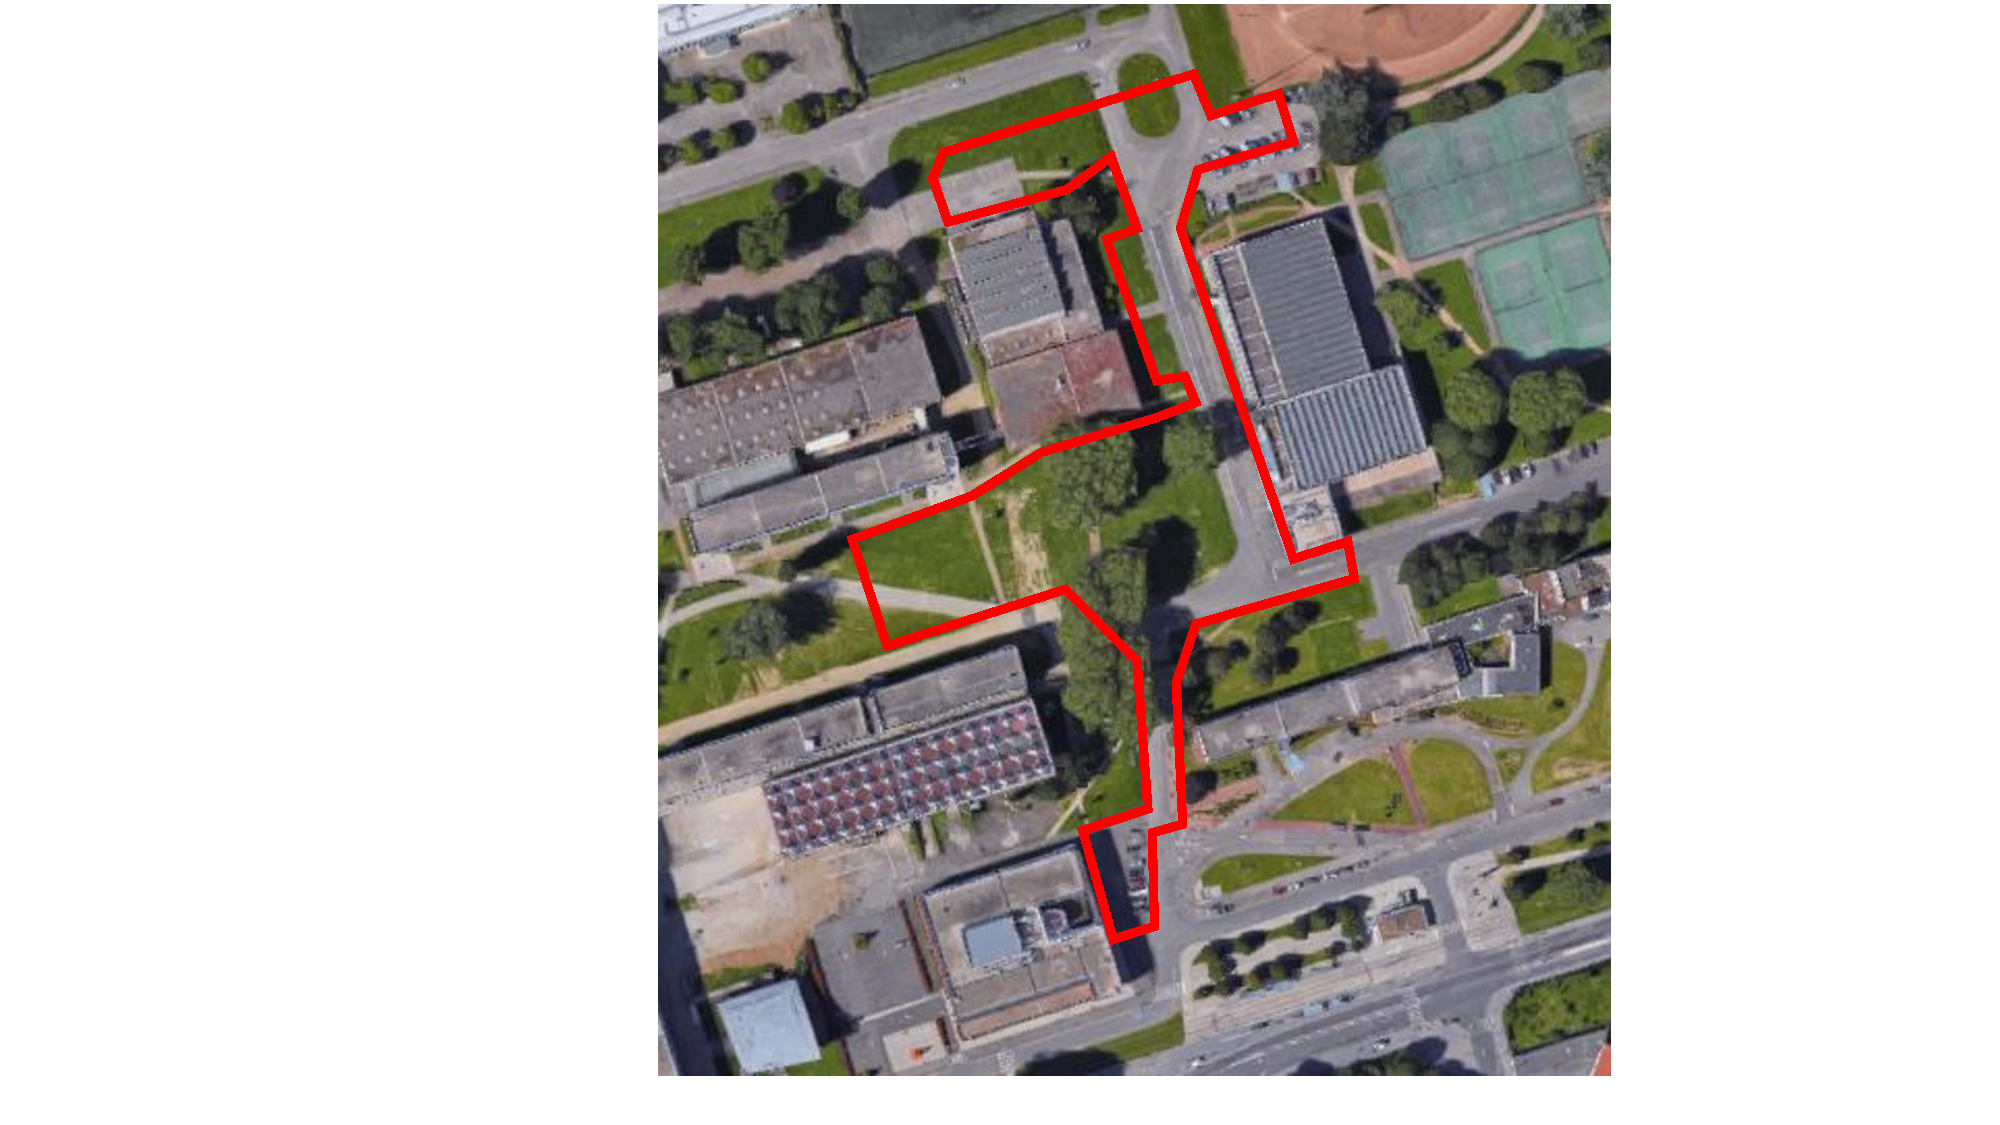
\includegraphics[width=.8\textwidth,keepaspectratio]{Exports/ERP_vue_aerienne.pdf}
	\captionof{figure}{Vue aérienne de la zone}
\end{center}
\newpage
\section{Photos de la zone (janvier 2017)}
\subsection{Zone nue}
\begin{center}
	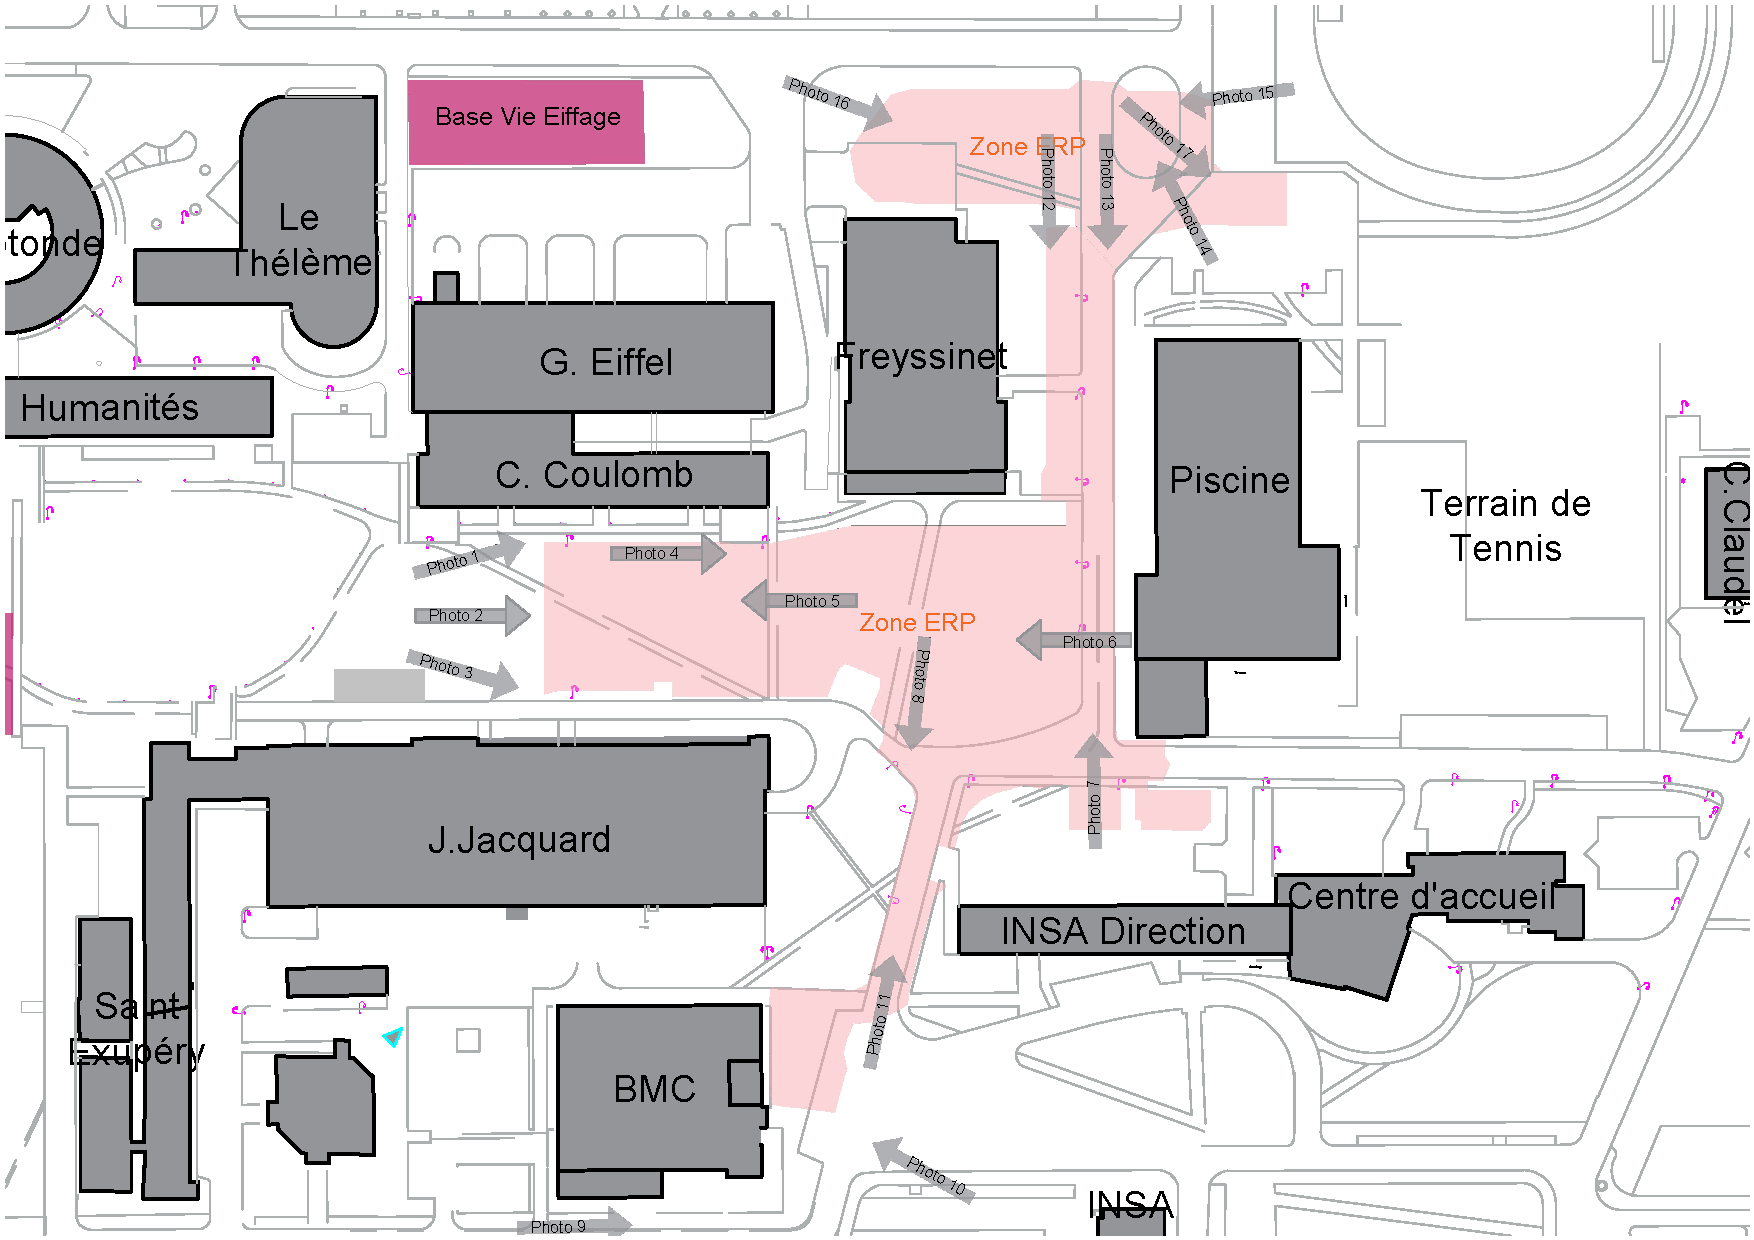
\includegraphics[angle=90,width=.8\textwidth,keepaspectratio]{Exports/Plan_24h_44eme-Photos_Zone}
	\captionof{figure}{Disposition des prises de vues de la zone nue}
\end{center}
\newpage

\begin{center}
\begin{tabular}{ll}
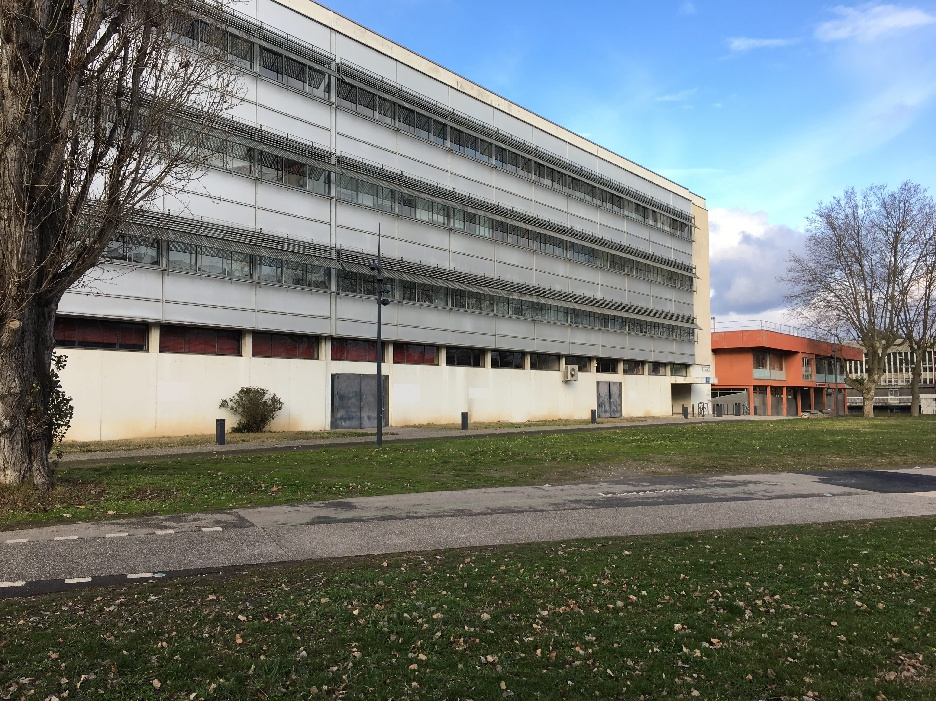
\includegraphics[width=.45\textwidth]{Annexes/Exports/Photo_1} & 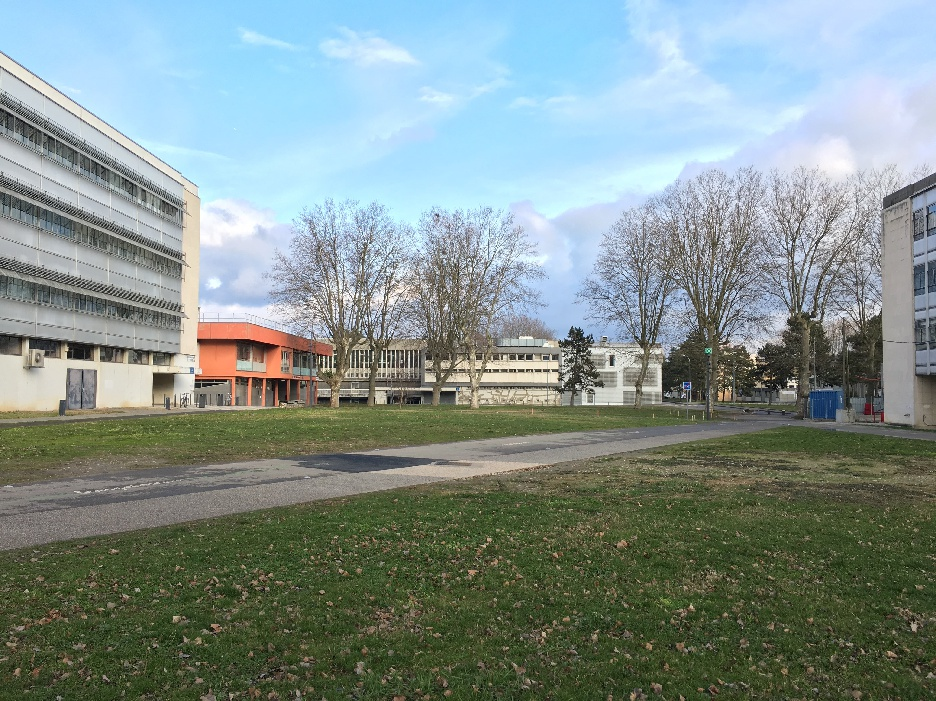
\includegraphics[width=.45\textwidth]{Annexes/Exports/Photo_2} \\
\textbf{Photo 1 :} Bâtiment Coulomb longeant la zone ERP & \textbf{Photo 2 :} Pelouse recevant l'ERP
\vspace{0.2 cm}\\
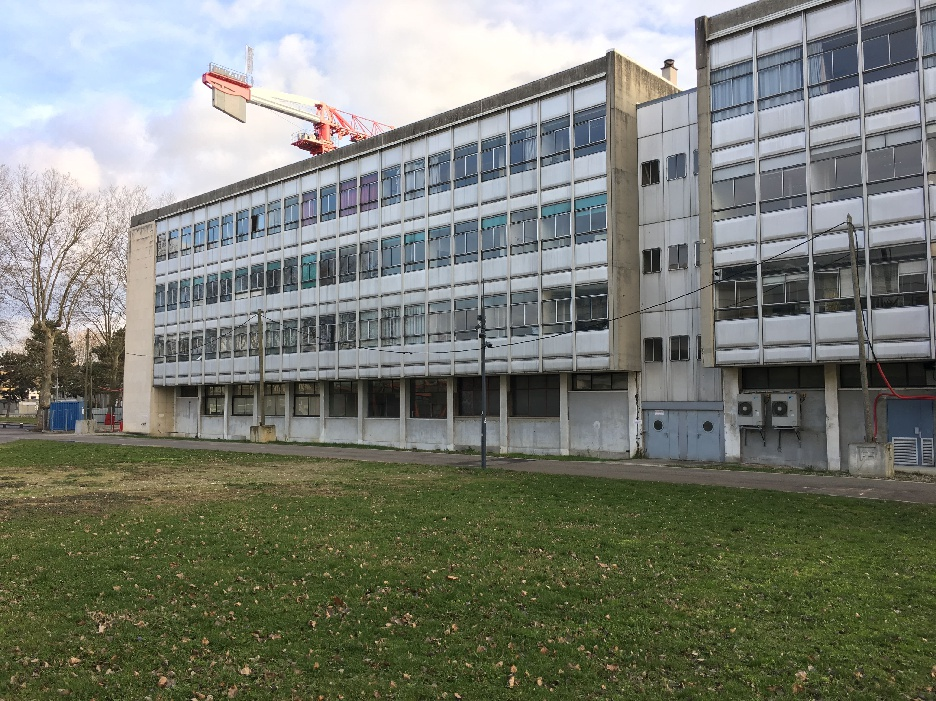
\includegraphics[width=.45\textwidth]{Annexes/Exports/Photo_3} & 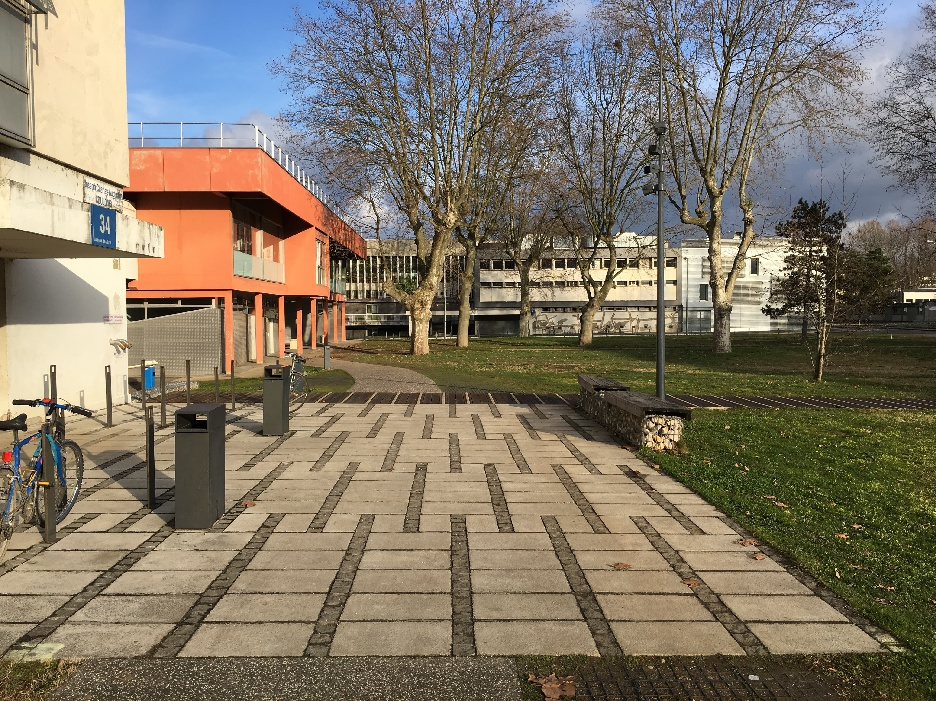
\includegraphics[width=.45\textwidth]{Annexes/Exports/Photo_4} \\
\textbf{Photo 3:}Bâtiment Jacquard longeant la zone ERP & \textbf{Photo 4 :} Voie pompier Coulomb
\vspace{0.2 cm}\\
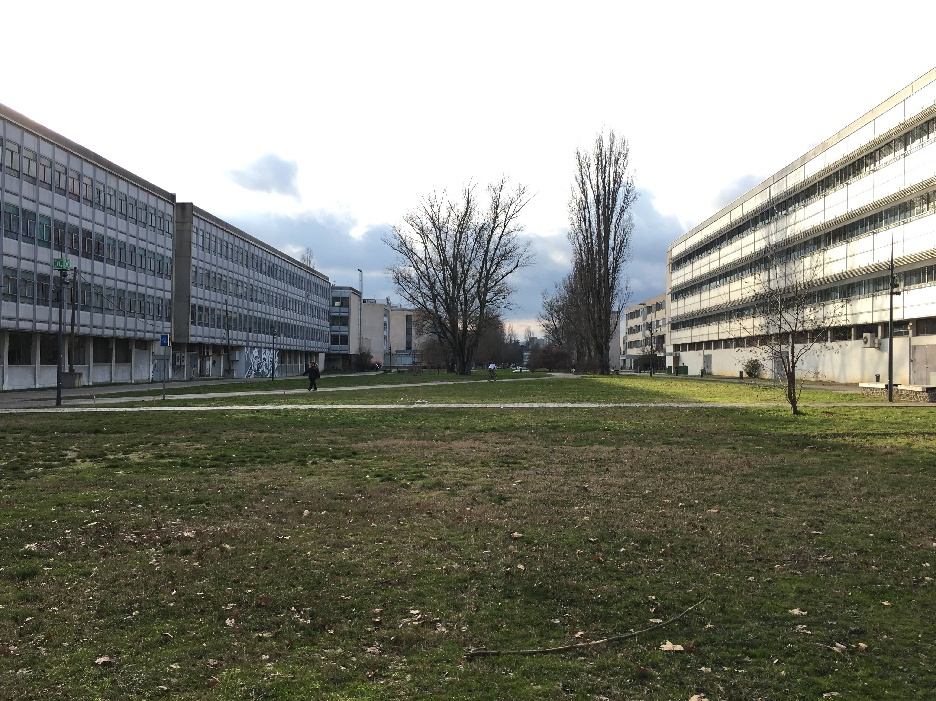
\includegraphics[width=.45\textwidth]{Annexes/Exports/Photo_5} & 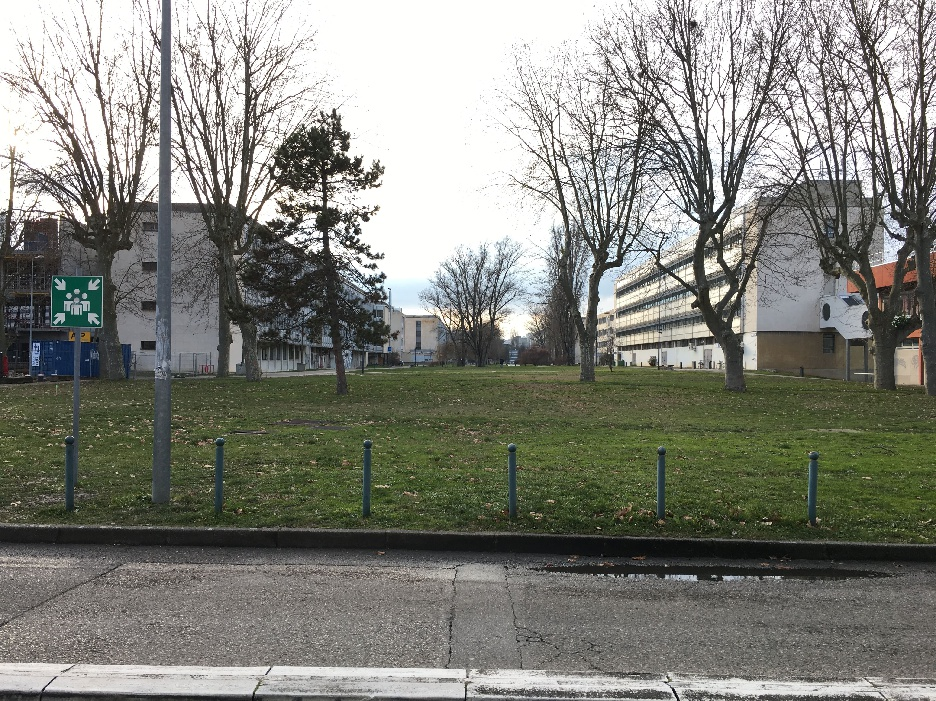
\includegraphics[width=.45\textwidth]{Annexes/Exports/Photo_6} \\
\textbf{Photo 5 :} Pelouse recevant la zone ERP & \textbf{Photo 6 :} Pelouse recevant la zone ERP\\
\end{tabular}
\end{center}

\newpage

\begin{center}
\begin{tabular}{ll}
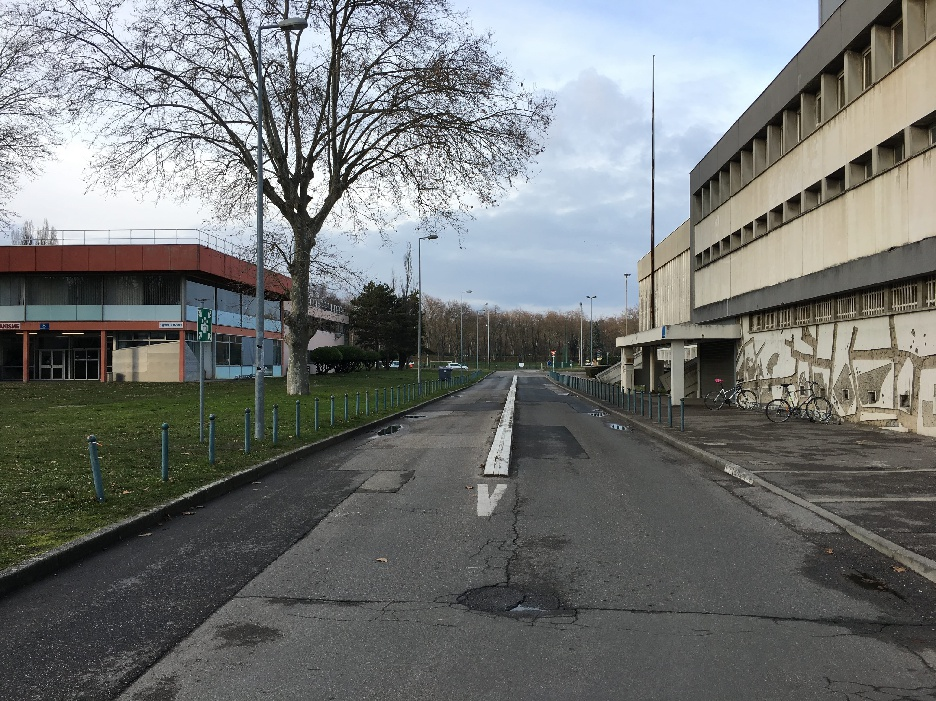
\includegraphics[width=.45\textwidth]{Annexes/Exports/Photo_7} & 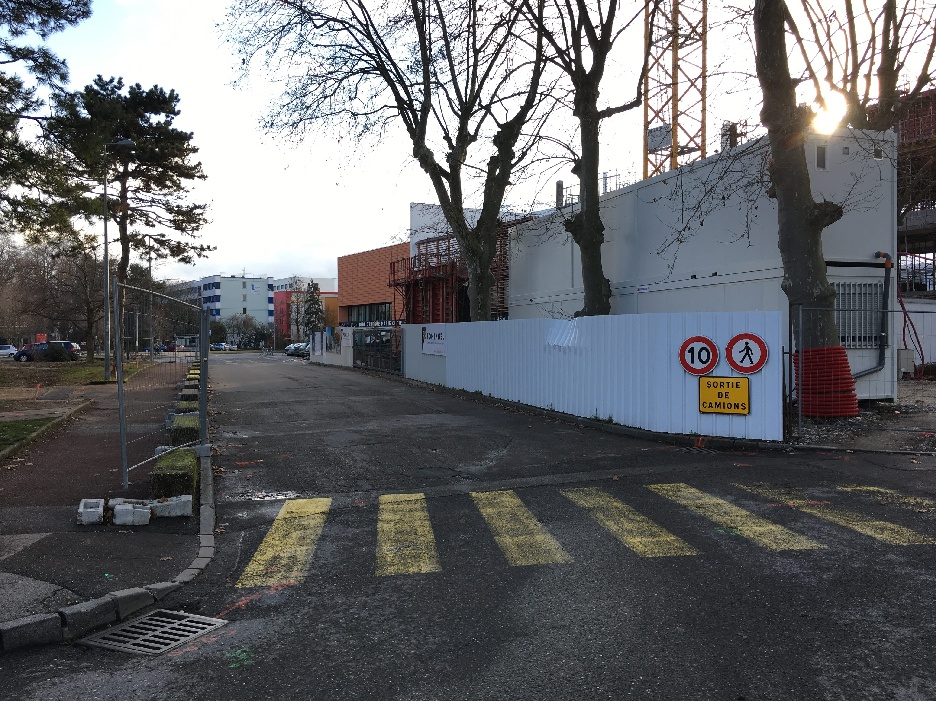
\includegraphics[width=.45\textwidth]{Annexes/Exports/Photo_8} \\
\textbf{Photo 7 :} Rue des Sports & \textbf{Photo 8 :} Rue des Sports - Sud
\vspace{0.2 cm}\\
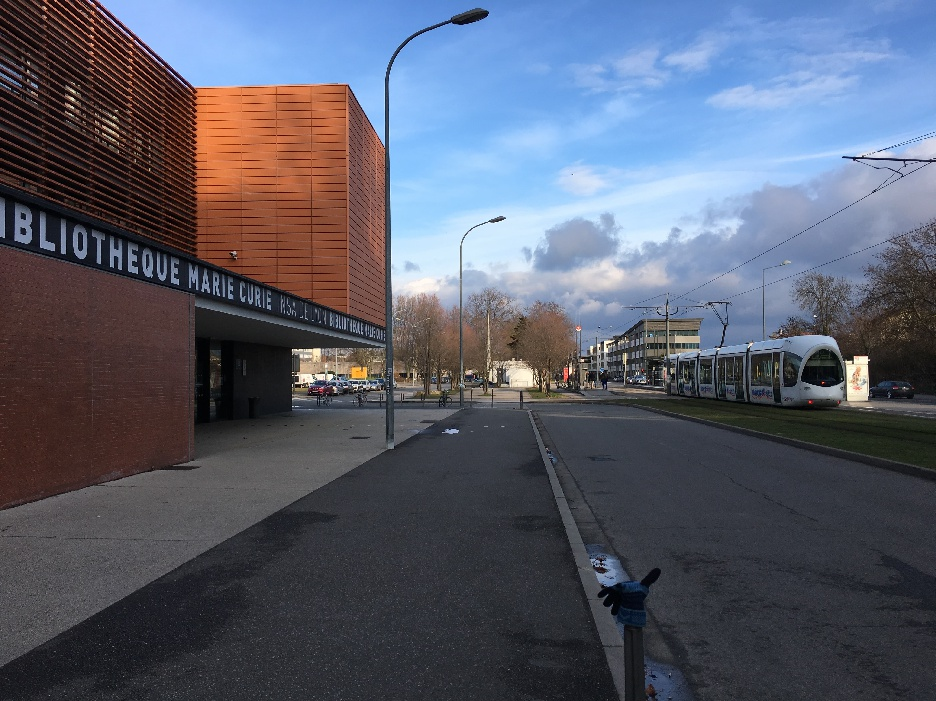
\includegraphics[width=.45\textwidth]{Annexes/Exports/Photo_9} & 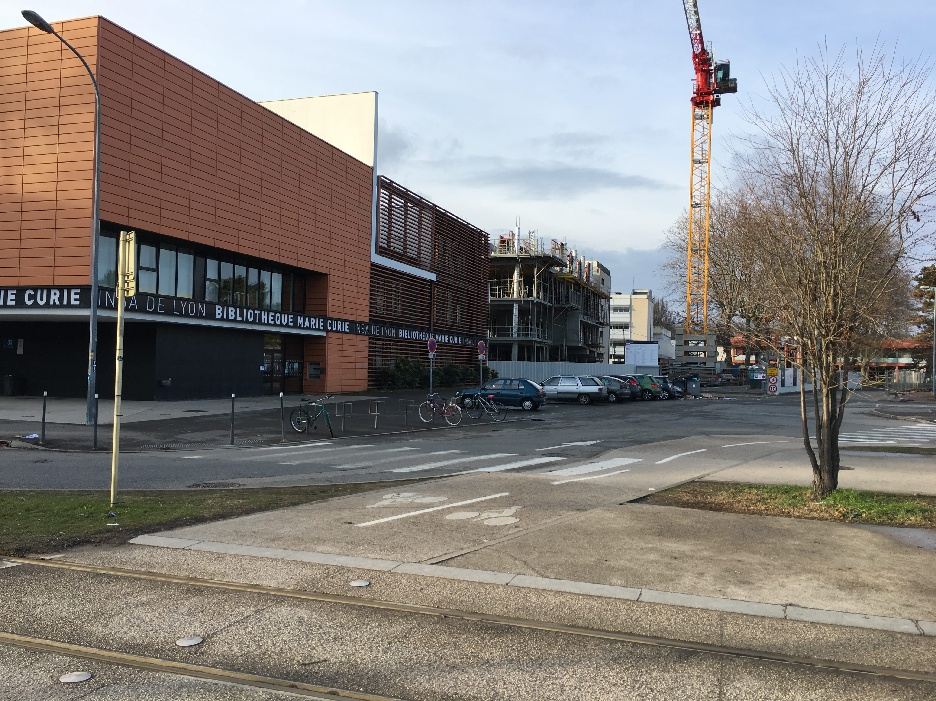
\includegraphics[width=.45\textwidth]{Annexes/Exports/Photo_10} \\
\textbf{Photo 9 :} Zone des caisses & \textbf{Photo 10 :} Zone des entrées
\vspace{0.2 cm}\\
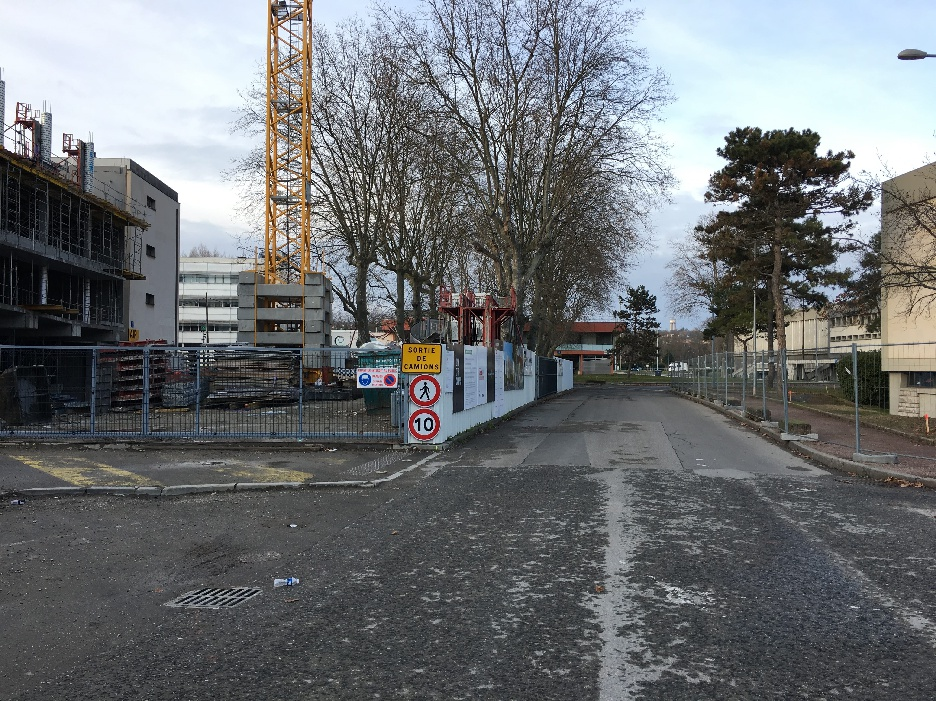
\includegraphics[width=.45\textwidth]{Annexes/Exports/Photo_11} & 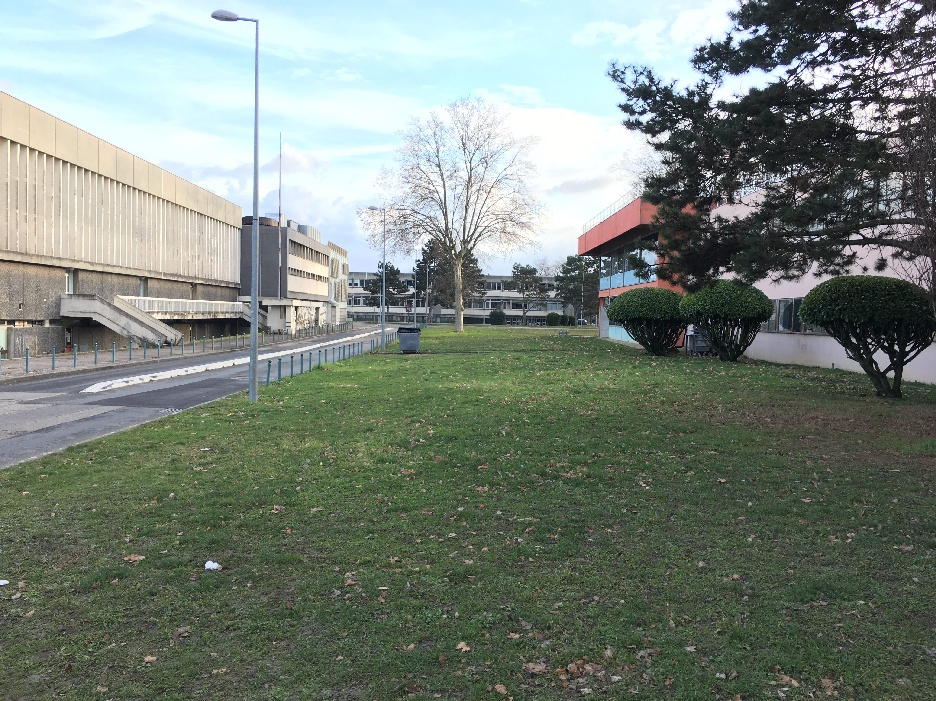
\includegraphics[width=.45\textwidth]{Annexes/Exports/Photo_12} \\
\textbf{Photo 11 :} Rue des Sports - Sud & \textbf{Photo 12 :} Espace Restauration\\
\end{tabular}
\end{center}

\newpage

\begin{center}
\begin{tabular}{ll}
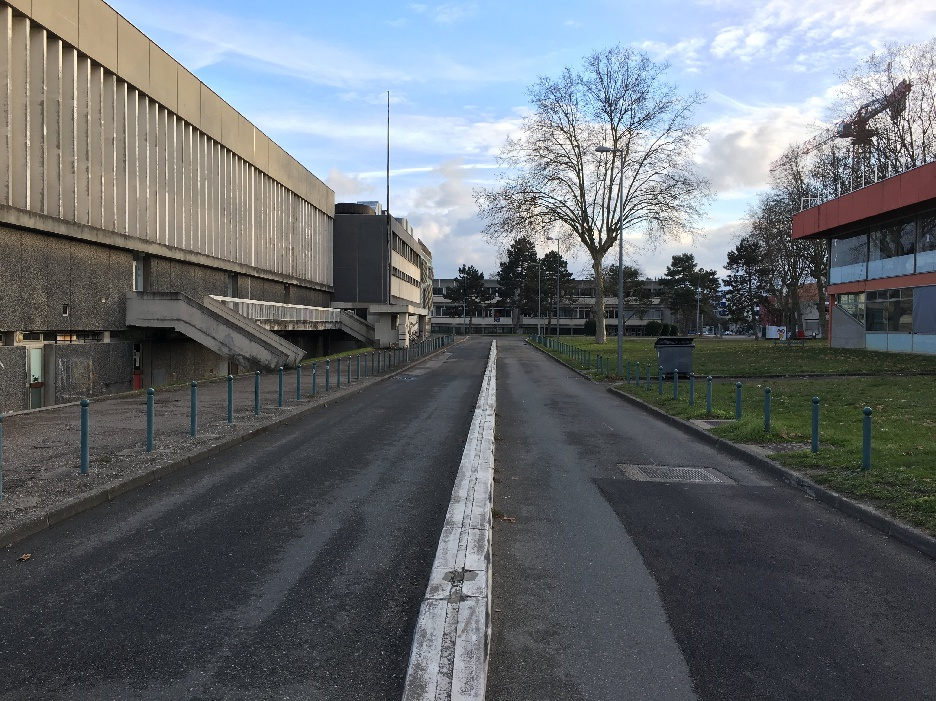
\includegraphics[width=.45\textwidth]{Annexes/Exports/Photo_13} & 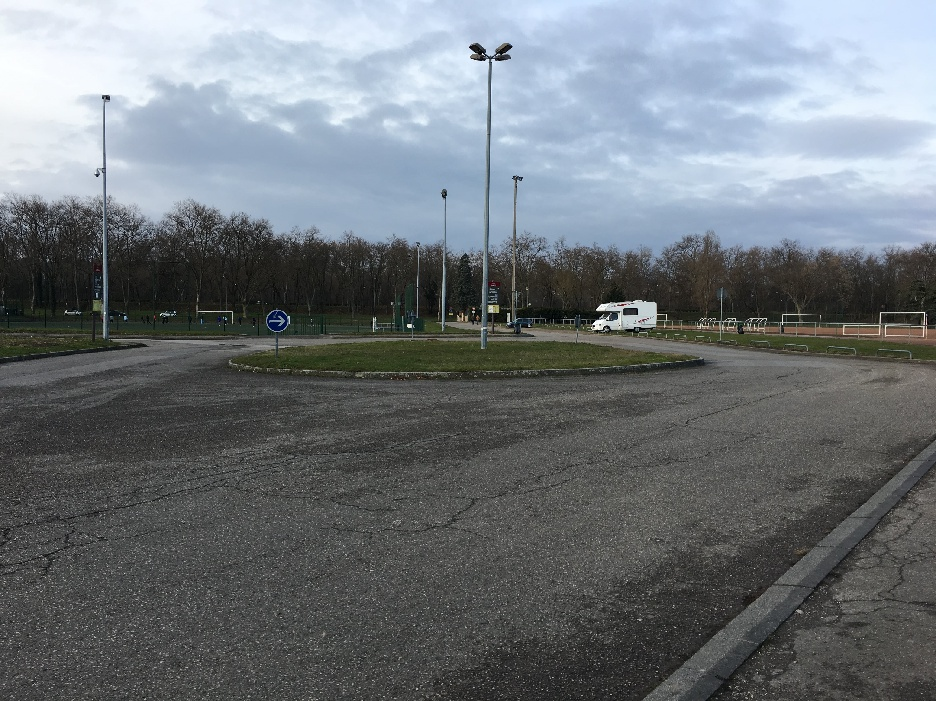
\includegraphics[width=.45\textwidth]{Annexes/Exports/Photo_14} \\
\textbf{Photo 13 :} Rue des Sports devant le Gymnase C & \textbf{Photo 14 :} Rond-point au nord de la zone
\vspace{0.2 cm}\\
\includegraphics[width=.45\textwidth]{Annexes/Exports/Photo_15} & \includegraphics[width=.45\textwidth]{Annexes/Exports/Photo_16} \\
\textbf{Photo 15 :} Pelouse recevant la zone ERP & \textbf{Photo 16 :} Pelouse recevant la zone ERP
\vspace{0.2 cm}\\
\includegraphics[width=.45\textwidth]{Annexes/Exports/Photo_17} &  \\
\textbf{Photo 17 :} Espace accueillant la scène Root's&\\
\end{tabular}
\end{center}

%\begin{center}
%	\includegraphics[angle=90,width=.7\textwidth,keepaspectratio, page = 1]{Annexes/Exports/Photos_zone}
%	\includegraphics[angle=90,width=.7\textwidth,keepaspectratio, page = 2]{Annexes/Exports/Photos_zone}
%	\includegraphics[angle=90,width=.7\textwidth,keepaspectratio, page = 3]{Annexes/Exports/Photos_zone}
%	\includegraphics[angle=90,width=.7\textwidth,keepaspectratio, page = 4]{Annexes/Exports/Photos_zone}
%	\includegraphics[angle=90,width=.7\textwidth,keepaspectratio, page = 5]{Annexes/Exports/Photos_zone}
%\end{center}
\subsection{Zone en configuration concerts}

\begin{center}
	\includegraphics[scale=0.8]{Annexes/Images/concert2}
\end{center}
\vspace{10mm}
\begin{center}
	\includegraphics[scale=10]{Annexes/Images/concert1}
\end{center}
\newpage

\section{Dispositions vis-à-vis des Établissements Recevant du Public en Plein Air}


Afin de nous conformer au règlement de sécurité (Règlement de sécurité du 25 juin 1980 modifié sur les dispositions générales, R 123.1 à 55 et R 111.19 du ministère de l’intérieur et suivant le Code de la Construction et de l’Habitation complété par l’Arrêté du 6 Janvier 1983) contre les risques d’incendie et de panique dans les établissements recevant du public (E.R.P.), nous détaillons ici nos dispositions article par article en faisant référence aux dispositions spécifiques des établissements recevant du public de type plein air.
\\\\
Nous faisons également référence par analogie aux dispositions spécifiques aux ERP de type  M (Magasins) pour la zone des caisses et aux dispositions du type N (Restaurants ou débits de boissons) pour la zone de restauration.
Ces zones ne sont pas des ERP indépendants, mais des zones incluses dans l’ERP de plein air pour lesquelles des dispositions supplémentaires ont été mises en place sur la base de la réglementation ERP existante pour les ERP à activités analogues.  

\subsection{Généralités}

\subsubsection{Établissements assujettis (P.A.1)}
Étant donné que nous recevons un public dont l’effectif est supérieur à 1500 personnes, nous correspondons à un établissement ERP de \textbf{1ère catégorie.} \\
De plus, il s’agit d’une zone de concerts temporaire extérieure sur un site naturel existant (le campus «Lyon Tech - La Doua»). La zone de concerts est donc un \textbf{ERP de type Plein Air.}

\subsubsection{Calcul de l’effectif (P.A.2)}
\label{calcul_de_leffectif} 

Étant donné que nous n’utilisons ni gradin ni tribune, nous pouvons accueillir sur les zones réservées aux spectateurs (à l’exclusion des dégagements) trois personnes stationnant debout par mètre carré ou cinq personnes par mètre linéaire. \\
D’après la superficie de la zone considérée (10 300 m²), nous pouvons accueillir \textbf{au maximum 30 900  personnes} à raison de 3 personnes par mètre carré.
Cependant la zone sera exploitée à hauteur de 10 000 personnes maximum comme les années précédentes.

\begin{center}
	\includegraphics[angle=90,width=.8\textwidth,keepaspectratio]{Exports/Plan_24h_44eme-Cotes}
	\captionof{figure}{Métré de la zone ERP}
\end{center}
\newpage
\subsection{Construction}

\subsubsection{Construction (P.A.3)} 
\label{refArticleERPContruction}
D’après l’implantation de la Zone de Concerts définie sur les plans, nous n’avons aucune installation dangereuse à moins de 10 mètres de la zone concernée. \\
De plus l’accès au périmètre de l’ERP peut se faire par 2 voies d’accès d’au moins 12 mètres de large : 
\begin{list}{•}{}
	\item Avenue des Arts ;
	\item Rue des Sports – Nord
\end{list}

Et 4 voies d’accès d’au moins 8 mètres de large : 
\begin{list}{•}{}
	\item Voie Pompier du capitaine PONS (via rue des humanités)
	\item Voie Pompier Coulomb
	\item Rue des Sports – Sud
	\item Rue des Sciences
\end{list}

\begin{center}
	\includegraphics[width=.8\textwidth,keepaspectratio]{Exports/Plan_24h_44eme-Acces_Pompiers}
	\captionof{figure}{Accès pompiers à l'ERP}
\end{center}

Le stationnement de véhicules sur l’ensemble de ces voies d’accès est strictement interdit pendant toute la durée de la manifestation. \\

Si les accès pompiers précédemment mentionnés sont entravés par des barrières, alors elles sont systématiquement et constamment gardées par des agents de sûreté ou des bénévoles de l’organisation pour ouvrir les accès aux moyens de secours.\\

\textbf{Remarques (CO4): }\\
Cette zone ERP est desservie sur au moins la moitié de son périmètre par les voies d’accès des services de secours. 

La façade nord est accessible par l’avenue des Arts et la rue des Sports – Nord. 

La façade sud est accessible par la rue des Sports – Sud, la rue des Sciences ainsi que par la voie du capitaine Pons. 

La façade ouest est quant à elle accessible par la voie pompier Coulomb.\\


\textbf{Remarques (CO8): }\\
Cinq bâtiments tiers sont situés en contact de la zone. Les bâtiments Freyssinet, Jacquard, Coulomb, Marie Curie et le Gymnase C sont séparés d’au moins 4 mètres de la zone ERP. 

Les fiches ERP de ces bâtiments sont disponibles en Annexe du présent dossier. 

Lors de la manifestation des 18, 19 et 20 mai 2018, ces bâtiments seront vides d’effectif public, seuls le PC sécurité, le poste de secours, l'espace VIP ainsi que les loges des artistes seront dans ces locaux. 


\subsubsection{Règles parasismiques (P.A.4)} 
Abrogées par arrêté du 10 novembre 1994. 
\subsubsection{Tribunes et gradins non démontables (P.A.5) } 
Notre installation ne comporte aucune tribune ni gradin.
\subsubsection{Locaux à risques particuliers (P.A.6)}
Notre installation ne comporte pas de locaux à risques particuliers.
\subsection{Dégagements}

\subsubsection{Escaliers, vomitoires, sorties des tribunes et gradins non démontables (P.A.7)}

Calcul du nombre de sorties et d’unités de passage (UP) 
\\
Pour nos calculs de dégagements, la capacité de l’esplanade retenue est \textbf{30 900 personnes.}

Pour les établissements de plus de 3 000 personnes, il faut prévoir 3 sorties et rajouter 1 sortie par tranche supplémentaire de 3 000 personnes, soit ici \textbf{13 sorties}.

De plus il faut prévoir une unité de passage par tranche de 300 personnes, soit ici \textbf{103 UP}. \\

\begin{center}
	Le dispositif propose :        \textbf{13 sorties – 113 UP}\\
	Pour un minimum de :         \textbf{13 sorties – 103 UP}
\end{center}
Soit un différentiel positif de \textbf{10 UP}. \\

\textbf{Répartition des sorties :}

Les sorties sont réparties équitablement autour de l’ERP :
\begin{list}{•}{}
	\item1 sortie de 3,5m (5UP) au sud de la Scène Nord (\textbf{A}) 
	\item2 sorties de 7m (22UP) et 1 sortie de 3,5m (5UP) sur l’avenue des Arts (\textbf{B}, \textbf{C} et \textbf{D})
	\item1 sortie de 7m (11UP) au sud du terrain stabilisé (\textbf{E})
	\item1 sortie de 3,5m (5UP) à proximité du poste de secours (\textbf{F})
	\item2 sorties de 7m (22UP) sur la rue des Sciences (\textbf{G} et \textbf{H})
	\item1 sortie de 7m (11UP) sur la rue des Sports - Sud (\textbf{I})
	\item1 sortie de 3,5m (5 UP) et 1 sortie de 7m (11UP) à proximité du bâtiment Jacquard (\textbf{J} et \textbf{K})
	\item1 sortie de 3,5m (5UP) au nord de la Grande Scène (\textbf{L})
	\item1 sortie de 7m (11UP) à proximité du bâtiment Coulomb (\textbf{M})
\end{list}

En aucun point de la zone le public ne se trouve à plus de 50 mètres d’une issue de secours, et les principales circulations d’évacuation sont détaillées ci-après. 

\begin{center}
	\includegraphics[width=1\textwidth,keepaspectratio, angle=90]{Exports/Plan_24h_44eme-IS}
	\captionof{figure}{Disposition des dégagements et circulations d’évacuation}
	\includegraphics[width=.8\textwidth,keepaspectratio, angle=90]{Exports/Plan_24h_44eme-Cercles}
	\captionof{figure}{Distance séparant les sorties et chaque lieu de la zone ERP}
\end{center}


\subsubsection{Ouverture des accès (P.A.8)}

Tous nos accès sont placés en permanence sous la surveillance d’un préposé. Les entrées du festival, les sorties des visiteurs et les sorties de secours sont en permanence gardées par un agent de sûreté qui ouvre ces dernières pour permettre le passage en cas d’évacuation.
\subsection{Aménagements intérieurs, décoration et mobilier}
\subsubsection{Rangées de sièges ou de bancs (P.A.9)}
Ne s'applique pas.
\subsection{Installations électriques (P.A.10)}
\label{InstallationsElectriques}
Les installations électriques sont vérifiées au préalable par le bureau de contrôle et de vérification réglementaire. 

Elles sont conformes à la norme \textbf{NFC 15-100}.

Aucune prise de courant sous tension ne sera à portée du public durant la manifestation.
\subsection{Éclairage (P.A.11)}
\label{Eclairage}
\subsubsection{Éclairage permanent}

Les appareils d’éclairage mobiles ou suspendus étant interdits, les projecteurs éclairant nos comptoirs boissons sont fixés à la structure métallique de ces derniers. Certains projecteurs seront solidement fixés dans des arbres.\\

L’exploitation se fait en nocturne. L’éclairage permanent de la zone et des sorties est assuré par l’éclairage public, par celui des comptoirs de boissons et celui des scènes. 

\subsubsection{Éclairage de sécurité}
Un éclairage de sécurité autonome par un système de blocs phares est mis en place afin d’assurer le balisage des dégagements en cas de coupure électrique : des projecteurs dotés de batteries sont disposés sur la structure métallique des régies et des scènes afin d’éclairer en cas d’urgence les 13 sorties. \\

Ces éclairages se mettent en route automatiquement suite à une coupure de l’alimentation et peuvent fonctionner pendant environ 30 minutes. 


\begin{center}
	\includegraphics[width=.8\textwidth,keepaspectratio]{Exports/Plan_24h_44eme-Blocs_Phares}
	\captionof{figure}{Disposition des éclairages de sécurité (en orange)}
\end{center}


\subsection{Moyens de secours contre l’incendie}
\label{moyensSecoursIncendie}
\subsubsection{Moyens d’extinction (P.A. 12)}

Des moyens d’extinctions sont présents dans tous les endroits présentant des risques particuliers d’incendie.\\
Nous disposons de 3 types d’extincteurs :
\begin{list}{•}{}
	\item (E) A eau : au niveau des espaces de vente, aux entrées et aux toilettes
	\item (C) A CO2 : à proximité d’installations électriques 
	\item (A) AFFF (Agent formant un film flottant) : à proximité d’hydrocarbures ou huile (ici uniquement au niveau des stands de restauration). Ce type d’extincteur remplace les extincteurs à poudre car il produit les mêmes effets mais évite la création d’un nuage de poudre.
\end{list} \mbox{}\\

Un stock de chacun des trois types d’extincteurs est gardé à proximité du PC sécurité. 

\begin{center}
	\includegraphics[width=.8\textwidth,keepaspectratio]{Exports/Plan_24h_44eme-Extincteurs}
	\captionof{figure}{\label{moyens_extinction}Disposition des moyens d'extinction}
\end{center}


\subsubsection{Service de sécurité incendie (P.A.13)}
\label{SecuIncendie}

L’article \textbf{PA 13} précise, en application de l’article \textbf{MS 45}, qu’un service de sécurité incendie peut être imposé, dans les établissements importants présentant des risques particuliers d'incendie ou de panique, ce qui est le cas de notre établissement. \\

Une équipe de \textbf{5 agents certifiés SSIAP 1, 2 agents certifiés SSIAP 2 et d’un agent certifié SSIAP3 (au PC Sécurité)} est présente sur le site de 20 h à 4 h les 18 et 19  mai, et de 20h à 23h le 20 mai 2018. \\
Un Poste de Commandement Incendie est présent dans la bibliothèque Marie Curie. \\

Un agent SSIAP 1 est présent en permanence sur l’emplacement réservé aux Personnes à Mobilité Réduite de la grande scène afin de les aider à se diriger vers les issues de secours en cas d’incendie. 
\begin{center}
	\includegraphics[width=.8\textwidth,keepaspectratio]{Exports/Plan_24h_44eme-SSIAP}
	\captionof{figure}{Disposition des agents de sécurité incendie SSIAP}
\end{center}

\subsubsection{Système d'alerte  (P.A.14)}
\label{systemeAlerteIncendie}

Nous sommes dotés d’une liaison avec les sapeurs-pompiers et la ville de Villeurbanne (cadre d’astreinte) par téléphone urbain au poste de sécurité de la manifestation, situé dans la bibliothèque Marie Curie. \\

Les pompiers, ainsi que le service Sécurité Civile de la Ville de Villeurbanne seront informés du dispositif lors de la réunion générale de sécurité. \\

De plus, un message sonore pré-enregistré est diffusable sur le système de sonorisation de chacune des scènes.

\section{Dispositions spécifiques}
\subsection{Dispositions spécifiques à la zone des caisses}
L’accès aux soirées de concerts des 24 heures de l’INSA est payant. Un espace dédié à la vente de billets est situé à l’entrée de la zone. \\
La zone des caisses est une zone dédiée uniquement à la vente de billets pour accéder à la zone principale. Elle est composée d'une file d’attente matérialisée à l’aide de barrières de police de type Vauban qui débouche sur un préfabriqué de caisse. A la suite de l'achat du billet, le festivalier accède aux files d'attente pour entrer dans la Zone de Concerts. Les festivaliers seront invités à acheter leurs billets en amont de la manifestation, et s'ils les achètent sur place à effectuer cet achat sur leur téléphone pour réduire l'affluence aux caisses.
\begin{center}
	\includegraphics[width=.8\textwidth,keepaspectratio]{Exports/Plan_24h_44eme-Entree}
	\captionof{figure}{Plan de la zone des caisses}
	\includegraphics[width=.8\textwidth,keepaspectratio]{Exports/Plan_24h_44eme-Entree_zoom}
	\captionof{figure}{Plan de la zone des caisses - détail}
\end{center}
\subsubsection{Calcul de l’effectif :}
Nous nous basons pour le calcul sur l’article PA 2. La superficie de la zone est de \textbf{496m²}. Elle peut donc accueillir \textbf{1488 personnes}. Les dispositions prises pour cette zone se basent donc sur la réglementation ERP plein air de \textbf{2e catégorie}. \\
\subsubsection{Calcul des dégagements:}
Cette zone a une capacité comprise entre 501 et 3000 personnes, nous devons donc prévoir \textbf{3 sorties} au minimum en accord avec l’article PA 7. De plus il faut prévoir une unité de passage par tranche de 300 personnes, soit ici \textbf{5 UP}. 
\begin{center}
	Le dispositif propose :        \textbf{11 sorties – 27 UP}
	
	Pour un minimum de :         \textbf{ 3 sorties – 5 UP}
\end{center}

\begin{center}
	\includegraphics[width=.8\textwidth,keepaspectratio]{Exports/Plan_24h_44eme-Entree_IS}
	\captionof{figure}{Évacuation de la zone des caisses}
\end{center}

De par sa nature d’espace de vente comportant des caisses, on peut se référer, par analogie, à la règlementation \textbf{ERP de type M}, et en particulier l’article M 9 qui définit la conception des dégagements pour des zones présentant des caisses groupées. \\

Nous disposons ici d’un groupe de 3 caisses côte à côte. \textbf{L’article M 9 §1 a)} du 21 juin 1982 prévoit qu’un groupe de moins de 10 caisses doit prévoir un dégagement à l’une de ses extrémités, de préférence du côté opposé au public, ce qui est notre cas :
\begin{center}
	\includegraphics[width=.8\textwidth,keepaspectratio]{Exports/Plan_24h_44eme-Entree_Degagements}
	\captionof{figure}{Dégagement au niveau du groupe de caisses}
\end{center}
De plus, l’article \textbf{M 9 §4 }du 2 février 1993 prévoit que les groupes de 1 à 20 caisses doivent prévoir un passage de 0,90m de largeur praticable aux Personnes à Mobilité Réduite. Ce passage est disposé comme présenté ci-dessous et sera signalé par un pictogramme normalisé. A la sortie, le cheminement utilisé par le public est adapté aux PMR. 

\begin{center}
	\includegraphics[width=.6\textwidth,keepaspectratio]{Exports/Plan_24h_44eme-Entree_PMR}
	\captionof{figure}{Circulation pour les PMR}
\end{center}


Une équipe d’agents de sûreté composée d’un SSIAP 1 sera chargée de prendre en charge les Personnes à Mobilité Réduite souhaitant utiliser les caisses en les guidant sur le parcours défini ci-dessus. 
\newpage

\subsection{Dispositions spécifiques à l’espace restauration}

\subsubsection{Plan de situation:}
L’espace restauration est situé à l'est du bâtiment Freyssinet. Il est composé de divers stands de restauration, ainsi que de "mange-debout", de tables et de bancs en plastique dans un espace délimité par des barrières  de police de type Vauban et des barrières de clôture de type Héras.

\begin{center}
	\includegraphics[width=.8\textwidth,keepaspectratio]{Exports/Plan_24h_44eme-Espace_Resto}
	\captionof{figure}{\label{refFigSituationRestauration}Plan de situation de l'espace restauration}
	\includegraphics[scale=0.45]{Exports/Plan_24h_44eme-Espace_Resto_zoom}
	\captionof{figure}{Plan de situation de l'espace restauration - détail}
\end{center}

\subsubsection{Calcul de l'effectif (Article N 2):}
La superficie totale de la zone de restauration est de \textbf{604 m\up{2}}. On peut, par analogie, se référer à la réglementation \textbf{ERP de type N} (Restaurants ou débits de boissons) pour évaluer l’effectif de la zone. \\

La réglementation de type N indique une densité de \textbf{1 personne/m\up{2}} en cas de restauration assise, \textbf{2 personnes/m\up{2}} en cas de restauration debout, et \textbf{3 personnes/m\up{2}} en file d'attente. Ici nous avons ces trois zones, répartie de la façon suivante :

\begin{list}{•}{}
	\item File d'attente : \textbf{408 m\up{2}}, soit 1224 personnes admissibles.
	\item Zone de restauration debout : \textbf{70 m\up{2}}, soit 140 personnes admissibles.
	\item Zone de restauration assise : \textbf{126 m\up{2}}, soit 126 personnes admissibles.
\end{list} \mbox{}\\

L'effectif total admissible dans cette zone est donc de \textbf{1490 personnes}. La zone accueillant plus de 200 personnes, nous nous référerons aux articles concernant les catégories 1 à 4. \\

\begin{center}
	\includegraphics[width=.8\textwidth,keepaspectratio]{Exports/Plan_24h_44eme-Espace_Resto_Cotes}
	\captionof{figure}{Métré et dégagements de l'espace restauration}
\end{center}

\subsubsection{Dégagements et évacuation:}
Par analogie avec la réglementation de type N, l’article \textbf{CO 38 §1} indique que pour les établissements recevant plus de 100 personnes, \textbf{deux dégagements jusqu’à 500 personnes doivent être prévus, auxquels vient s'ajouter un dégagement par tranche de 500 personnes supplémentaires}. De plus, il est indiqué que \textbf{la largeur des dégagements doit être calculée à raison d'une unité de passage pour 100 personnes ou fraction de 100 personnes}, ce qui donne 15 unités de passage dans notre cas. \\

Etant donné la configuration de notre zone, nous ne pourrons mettre en place qu'un maximum de trois sorties, réparties sur toute la façade est de l'espace de restauration. En revanche, nous avons un total de \textbf{22 UP}, pour un minimum de 15 UP, soit un \textbf{différentiel positif de 7 UP}. 

\subsubsection{Eclairage:}

Conformément aux \textbf{articles EC 7 à 15}, un éclairage de sécurité sera mis en place, tel qu'on peut le voir sur la figure précédente.

\subsubsection{Moyens de secours contre l'incendie:}

Les moyens secours contre l'incendie mis en oeuvre sont tels que décrit au paragraphe \ref{moyensSecoursIncendie}.

\subsubsection{Mobilier:}
Le mobilier utilisé sera fourni par la mairie de Villeurbanne. Il sera composé de tables et de bancs en plastique. 
\begin{center}
	\includegraphics[scale=1]{Annexes/Images/tables}
	\captionof{figure}{Type de mobilier utilisé sur l'espace restauration}
\end{center}
La réglementation de type N n’impose pas de résistance au feu pour le mobilier dit “courant” dont font partie les tables et les bancs. \\

\subsubsection{Sûreté:}

La zone de restauration sera placée sous le contrôle de \textbf{2 agents de sûreté}, placés au niveau des accès à la zone, ainsi que d'un agent supplémentaire au niveau du bar PMR. Ils auront pour mission de s'assurer du maintien de l'ordre dans cette zone.

\subsection{Dispositions spécifiques à l'espace Scène Root's}
\label{Scene_roots}
\textbf{Présentation du principe:}\\

La Scène Root's est une petite scène, sur laquelle sera diffusée de la musique d'un genre alternatif aux deux autres scènes. Elle sera constituée d'un podium formé par des praticables de la mairie de Villeurbanne, et recouverte par une bache tendue par deux arches, tel que vous pouvez le voir sur l'image suivante :

\begin{center}
	\includegraphics[width=.8\textwidth,keepaspectratio]{Annexes/Images/SceneRoots}
	\captionof{figure}{Schéma 3D de la structure de la Scène Root's}
\end{center}

Les arches circulaires ont un diamètre de 6 mètres et sont espacés de 7 mètres. Le podium sera de 6 par 4 mètres, à une hateur de 80 cm. La hauteur totale sera de 4 mètres.\\

Au dessus du public seront tendues, à l'aide de six totems, des voilures en lycra ignifugé. Elles auront une fonction décorative. Les cinq totems périphériques feront 4 mètres de haut, seront en dehors de la zone accessible au public et lestés par des blocs en béton. Le sixième fera 6 mètres et se trouvera au centre, lesté par une embase lourde de 60 kg. Il sera aussi maintenu en place grâce à l'haubanage avec les autres totems. Afin d'empêcher au public de monter sur le totem accessible, des planches bloqueront l'accès aux barreaux sur une hauteur suffisante. 

\begin{center}
	\includegraphics[width=.8\textwidth,keepaspectratio]{Annexes/Images/Totems}
	\captionof{figure}{Schéma 3D de la répartition des totems}
\end{center}

La résistance au vent et les charges maximales feront l'objet d'une note de calcul à venir.\\

Cette animation aura lieu :
\begin{list}{•}{}
	\item le vendredi \textbf{18} mai de \textbf{20h à 3h20}
	\item le samedi \textbf{19} mai de \textbf{13h à 17h} et de \textbf{20h à 3h20}
	\item le dimanche \textbf{20} mai de \textbf{13h à 17h}
\end{list}

\subsubsection{Implantation:}
Cette animation sera placée sur le parking au nord de la piscine.
\begin{center}
	\includegraphics[width=.8\textwidth,keepaspectratio]{Exports/Plan_24h_44eme-3e_Scene}
	\captionof{figure}{Implantation de l'animation "Scène Root's"}
\end{center}

\subsubsection{Réglementation:}
La zone de cette animation n'a pas de démarquation physique avec le reste de la zone ERP. Cependant, afin d’anticiper au mieux les risques liés à cette animation, nous reprenons ci-après, et \textbf{par analogie}, les différents articles de la réglementation PA sur lesquels nous nous sommes basés pour dimensionner le dispositif de sécurité. 

\newpage

\paragraph{Généralité}
\subparagraph*{Calcul de l'effectif (Article P.A.2):}\mbox{}\\
L’effectif maximal est dépendant du type d’activité qui y est pratiqué. Dans notre cas, la zone sera utilisée pour une animation musicale avec des spectateurs en plein air, ce qui rentre dans la catégorie PA. \\

L’article P.A.2 des dispositions spéciales pour le type PA indique un effectif maximal de 3 personnes/m\up{2}  pour les “personnes stationnant debout sur des zones réservées aux spectateurs”, ce qui est le cas pour l’animation Scène Root's. \\

La surface accessible au public étant de \textbf{206 m\up{2}}, la capacité maximale de la zone est donc de \textbf{618 personnes}. Nous nous situons dans la \textbf{troisième catégorie}. \\



\begin{center}
	\includegraphics[width=.75\textwidth,keepaspectratio]{Exports/Plan_24h_44eme-3e_Scene_Circ_Autour}
	\captionof{figure}{Circulations autour de la zone de l'animation}
\end{center}

\paragraph{Construction}

\subparagraph*{Implantation (Article P.A.3):}\mbox{}\\
La zone d’implantation ne présente pas de risque d’inflammation rapide (asphalte) et aucune installation dangereuse ne se trouve à moins de 20 mètres.

Deux voies de 8m de large (la rue des Sports Nord et Sud) desservent la facade ouest de la zone, conformément à l'article CO 4 cité dans l'article P.A.3.

\subparagraph*{Règles parasismiques (Article P.A.4) :}\mbox{}\\
Abrogé par arrêté du 10 novembre 1994.

\subparagraph*{Tribunes et gradins non démontables (Article P.A.5):}\mbox{}\\
Aucun gradin ni tribune ne sera installé dans cette zone.

\subparagraph*{Locaux à risques particuliers (Article P.A.6):}\mbox{}\\
Aucun local à risque particulier ne sera installé dans cette zone.

\paragraph{Dégagements}

\subparagraph*{Escaliers, vomitoires, sorties des tribunes et gradins non démontables (Article P.A.7):}\mbox{}\\
D’après la réglementation de l’article P.A.7, l’établissement ayant un effectif total admissible compris entre 501 et 3000 personnes, trois sorties doivent être prévues. De plus, le nombre d'unités de passage nécessaire pour accueillir 618 personnes s'élève à trois.
La configuration de cette zone nous permet de mettre en place un maximum de deux sorties seulement. En revanche, le nombre d'unités de passage est de \textbf{26}, soit un \textbf{différentiel positif de 23 UP}. De plus, la distance maximale séparant le public d'une sortie est de 12m.

\begin{center}
	\includegraphics[width=.8\textwidth,keepaspectratio]{Exports/Plan_24h_44eme-3e_Scene_Cotes}
	\captionof{figure}{Métré et dégagements de la zone}
\end{center}
\subparagraph*{Ouverture des accès (Article P.A.8):}\mbox{}\\
La sortie à l'ouest de la zone sera ouverte en permanence. Celle située à l'est sera gardée par un agent de sûreté de la société STAFF pendant toute la durée de l'exploitation.

\paragraph{Aménagements}

\subparagraph*{Rangées de sièges ou de bancs (Article P.A.9):}\mbox{}\\

Aucun mobilier, table, chaise, banc ne sera installé dans la zone accessible au public.

\paragraph{Electricité}

\subparagraph*{Installations électriques (Article P.A.10) :}\mbox{}\\

Identique aux dispositions décrites au paragraphe \ref{InstallationsElectriques}.

\subparagraph*{Éclairage (Article P.A.11):}\mbox{}\\

Identique aux dispositions décrites au paragraphe \ref{Eclairage}.

\subparagraph*{Moyens d'extinction (Article P.A.12):}\mbox{}\\

Deux extincteurs de type "Eau" et "CO2" seront placés à proximité de la scène.

\subparagraph*{Service de sécurité incendie (Article P.A.13):}\mbox{}\\

Comme spécifié au paragraphe \ref{SecuIncendie}, un agent certifié SSIAP 1 sera présent sur cette scène pendant son exploitation nocturne. \\

\subparagraph*{Système d'alerte (Article P.A.14):}\mbox{}\\

Identique aux dispositions décrites au paragraphe \ref{systemeAlerteIncendie}.

\begin{center}
	\includegraphics[width=.8\textwidth,keepaspectratio]{Exports/Plan_24h_44eme-3e_Scene_Secu_Incendie}
	\captionof{figure}{Disposition des moyens de lutte contre l'incendie dans la zone}
\end{center}

\newpage 

\subsection{Dispositions spécifiques à la zone ERP réduite le dimanche soir}

\textbf{Présentation du principe:}\\
Des concerts de jazz auront lieu sur la grande scène en clôture du festival le dimanche soir. Les deux concerts seront encadrés par les mêmes techniciens professionnels que pour les soirées du vendredi et du samedi.\\

La soirée du dimanche est destinée aux étudiants du campus, et la communication sera limitée en dehors des étudiants concernant cette soirée. Nous fixons donc une jauge maximale à \textbf{2 000 personnes}. Le nombre d'entrées sera compté par un bénévole à l'aide d'un compteur manuel. Passé ce seuil, l'accès à la zone ne sera plus autorisé.\\

Une zone ERP réduite sera mise en place à partir de 20h00 dans la partie sud de la Zone de Concerts.\\

Cette zone a une \textbf{capacité} comprise entre \textbf{501 et 3000 personnes}, nous devons donc \textbf{prévoir 3 sorties au minimum} en accord avec l’article P.A. 7. De plus il faut prévoir une unité de passage par tranche de 300 personnes, \textbf{soit ici 6 UP.}\\

La zone \textbf{comportera 6 sorties et 60 UP.} Soit un différentiel positif de \textbf{3 sorties et 54 UP.}\\
					
Les issues de secours et les unités de passage sont en conséquence modifiées comme indiquées sur la figure suivante.\\

En revanche, la disposition des extincteurs, éclairages de secours et installations électriques reste inchangée.\\

\begin{center}
\includegraphics[width=\textwidth,keepaspectratio, angle=90]{Exports/Plan_24h_44eme-Dimanche_IS}
\captionof{figure}{Issues de secours et dégagements du dimanche soir}
\end{center}

\newpage

\section{Annexes - Sécurité Incendie}
\subsection{Plan d'installation de la grande scène}
Note : la scène de l’édition 2018 ne sera plus identique aux éditions précédentes. Afin d'agrandir la surface utile ainsi que la résistance au vent, nous ferons appel à un prestataire différent. La structure utilisée permettra ainsi une résistance aux vents jusqu'à \textbf{110 km/h}.
\begin{center}
	\includegraphics[scale=0.40, angle=90]{Annexes/Images/GrandeScene}
	\captionof{figure}{\label{Grande_scene}Grande scène perspective 3D}
\end{center}

\subsection{Plan d’installation de l'arche d’entrée}
Ceci est l'arche qui surplombe les files des entrées. Elle permet l'accrochage de signalétique et de spots lumineux.
\begin{center}
	\includegraphics[scale=0.6, angle=90]{Annexes/Images/ArcheEntrees}
	\captionof{figure}{Arche vue perspective 3D}
\end{center}

\newpage

\subsection{Avis favorable du bureau de contrôle SOCOTEC}
L'établissement ERP tel que décrit jusqu'à présent a fait l'objet en 2017 d'un examen par le bureau de contrôle SOCOTEC et y a reçu un avis favorable.

\begin{center}
	\includegraphics[width=.75\textwidth,keepaspectratio]{Annexes/Documents/ERP2017AvisSOCOTEC}
	\captionof{figure}{Avis favorable du bureau de contrôle SOCOTEC}
\end{center}

\newpage

\subsection{Arrêté municipal autorisant le déroulement des concerts}

A venir. 

\newpage

\subsection{Autorisation du déroulement des concerts par la direction de l’INSA Lyon}
\begin{center}
	\includegraphics[scale=0.70]{Annexes/Documents/INSAAutorisationConcerts}
	\captionof{figure}{Autorisation du déroulement des concerts par la direction de l’INSA}
\end{center}

\subsection{Procès-verbal et rapport de la Sous-Commission Départementale de Sécurité des ERP/IGH de 2017}
\begin{center}
	\includegraphics[width=.75\textwidth,keepaspectratio,page=1]{Annexes/Documents/Proces_Verbal_SCDS_2017}
	\captionof{figure}{Avis favorable de la SCDS ERP-IGH pour l'édition 2017}
\end{center}

%------------------------------------------------------------------------------------------------------
%SURETE ET RISQUES
%------------------------------------------------------------------------------------------------------

\chapter{Sûreté et risques}
\section{Dispositions générales}
\subsection{Diagnostic de sûreté – Description de l’environnement}
Le but de cette partie est de définir le contexte dans lequel s’inscrit la manifestation. Elle met en avant les zones à risques et les comportements pouvant entraîner des problèmes. Parallèlement sont présentées les mesures planifiées pour répondre à ces risques.

\subsubsection{Diagnostic}
\paragraph{Locaux universitaires et laboratoires de recherche}
Le campus Lyon Tech - La Doua, premier centre de recherche scientifique et de formation de Lyon, accueille de nombreux laboratoires de spécialisations diverses (biochimie, nucléaire, tribologie, vibrations acoustiques, imagerie médicale, etc.). Certains d’entre eux gardent des produits présentant une dangerosité plus ou moins importante, parmi lesquels produits chimiques, gaz spéciaux, étouffants, toxiques ainsi que du matériel tel que des lasers, générateurs de rayons X…\\

Par ailleurs, dans les laboratoires comme dans les bâtiments d’enseignement, quel que soit le type de recherche effectuée, le matériel de valeur (matériel informatique ou équipements technologiques) qui s'y trouve augmente sensiblement les probabilités d’effraction et de vol dans ces bâtiments. 

\paragraph{Habitations et résidences universitaires}
En plus des bâtiments de cours et des laboratoires, de nombreuses résidences étudiantes sont localisées sur le campus, et un certain nombre d’habitations privées accueillent des membres du personnel et leur famille.\\
En tout, plus de 2 700 étudiants sont logés cette année dans 11 résidences à l’INSA, ainsi que 18 BIATOSS (Bibliothécaires, ingénieurs, administratifs, techniciens, ouvriers, personnels de service et de santé).

\subsubsection{Dispositions existantes}
\paragraph{Propres au campus}
En semaine comme le week-end, les bâtiments de l’INSA sont sous la surveillance du service de gardiennage de l’INSA, dont les équipes patrouillent jour et nuit. Le rôle principal de cet organisme, relié aux différents systèmes d’alarme et de vidéosurveillance des bâtiments, est de prévenir les éventuelles effractions en effectuant des rondes. Ils interviennent en cas d’intrusion et sont en liaison directe avec les services de police de Villeurbanne. \\

En ce qui concerne l’Université Claude Bernard et l’IUT Lyon 1, des services similaires existent, ceux-ci ayant pour mission de surveiller les bâtiments et notamment les laboratoires. Chacun de ces services a une bonne connaissance du terrain surveillé, liée à l’expérience qu’ils en ont respectivement.

\begin{center}
	\includegraphics[width=.8\textwidth]{Annexes/Plans/planDeSituation}
	\captionof{figure}{Plan de situation des bâtiments présents sur le campus LyonTech/La Doua}
\end{center}

\paragraph{Dispositions extérieures}
En cas de problème ne pouvant être géré directement par les services de sécurité, le campus accueille d’une part plusieurs infirmeries, et d’autre part bénéficie de la proximité appréciable de la police municipale de Villeurbanne, du centre des pompiers et de la clinique du Tonkin.
\begin{center}
	\includegraphics[scale=0.6]{Annexes/Plans/centreSecours}
	\captionof{figure}{Situation des centres de secours de Villeurbanne}
\end{center}
\newpage
\subsection{Organisateurs et bénévoles}

\subsubsection{Répartition des effectifs}
La répartition hiérarchique des effectifs est la suivante :
\begin{list}{•}{}
	\item 1 Président *
	\item 2 Responsables sécurité (au PC sécurité) *
	\item 2 Responsables Bénévoles
	\item 3 Responsables Logistique *
	\item 1 Responsable Billetterie *
	\item 3 Responsables Concerts *
	\item 2 Responsables Bars *
	\item 2 Responsables Catering
	\item 2 Responsables Logistique barrières
	\item 1 Responsable Signalétique
	\item 1 Responsable Décoration
	\item 1 Régisseur général et 6 techniciens s’occupant des scènes *
	\item 2 Electriciens *
	\item 7 Chefs d’équipe dirigeant les buvettes et divers stands *
	\item 300 Bénévoles répartis sur l’ensemble de la Zone de Concerts ayant pour missions principales les ventes, la prévention et le ramassage des déchets
\end{list}

\textit{* ces organisateurs ont été sensibilisé à l'utilisation des extincteurs}

\subsubsection{Coordination des effectifs}
\label{coordination_effectifs}

Les organisateurs sont conscients de l’enjeu de sécurité et de sûreté que représentent les 24 heures sur le campus. Ainsi le projet repose sur une organisation humaine cohérente qui facilite la sécurité. Les missions de chaque intervenant sont clairement définies en amont de la manifestation.

\begin{center}
	\begin{tabular}{ | p{6cm} | p{10cm} | }
		\hline
		\cellcolor[gray]{0.9}
		Acteurs & \cellcolor[gray]{0.9} Rôle \\ \hline
		Responsables sécurité des 24h :
		
		Valentin \textsc{Godrie}, \newline
		Léo \textsc{Mouyna} & Coordonner le dispositif de sécurité. Interlocuteurs privilégiés avec STAFF Sécurité, la Croix Rouge Française, les services de Gardiennage INSA et UCBL, le SAMU et les  pompiers. \\ \hline
		Président des 24h :
		
		Arthur \textsc{Saunier} & Interlocuteur privilégié des 24 heures de l'INSA avec les services de police, la mairie et la préfecture. \\ \hline
		Bénévoles & Accueil du public, relais des informations sur le terrain. \\ \hline
		Bénévoles dédiés à la surveillance & Bénévoles qui ne sont pas en contact avec le public et qui ont pour rôle de signaler les présences non-autorisées de personnes sur les différentes zones. \\ \hline
		Société privée (STAFF Sécurité) & Protection des participants et des équipements, palpations de sécurité, gestion de la foule.
		Jusqu’à 84 agents présents simultanément sur le campus. \\ \hline
		Secouristes (Croix-Rouge Française) & Premiers secours, assistance aux blessés, recensement des interventions.
		Jusqu’à 38 secouristes présents simultanément. \\ \hline
		Services de gardiennage
		(INSA et UCBL) & Protection des bâtiments. \\ \hline
		Secours
		(Pompiers, Samu, Police) & Secours, prise en charge du PMA. \\ \hline
		Mairie, Préfecture & Prise en charge des opérations en cas de situation de crise. \\ \hline
	\end{tabular}
\end{center}

La coordination du dispositif de sécurité est réalisée par les responsables sécurité et le président des 24 heures de l’INSA. Leur rôle est de centraliser toutes les informations remontant des équipes de bénévoles et de prendre les décisions qui s’imposent, en accord avec la société de sûreté et les secouristes.\\

Il est demandé à l’ensemble des bénévoles de faire remonter des informations complètes (lieu précis, type de problème identifié, nombre de personnes concernées). Les responsables sécurité et les bénévoles postés aux points de sécurité sont en liaison permanente par talkie-walkie. \\

De plus, des lignes de téléphones urbains sont à disposition dans la bibliothèque Marie Curie, où se trouve le PC sécurité. \\
Au moins un responsable sécurité sera présent dans ce PC sans discontinuité. A tout instant, les responsables sécurité, ainsi que le président, seront joignables.\\

Les responsables de la Croix Rouge possèdent également un talkie-walkie sur la fréquence des bénévoles et peuvent communiquer en interne sur une fréquence dédiée. \\

Les numéros des responsables sécurité, ainsi que celui du président, se trouvant au début du présent dossier, sont communiqués à tous les intervenants le jour de la réunion de sécurité. Ils sont également communiqués à tous les organisateurs et bénévoles par voie écrite et orale lors du «briefing bénévoles», qui a lieu lors de la semaine précédant la manifestation. Pendant ce briefing sont également précisés les procédures et les points de vigilance importants pour la sécurité.\\

\subsection{Emplacement du PCO et des PMA}
\label{refProcedurePMA}

En cas d’activation du Plan NOVI (Nombreuses Victimes) par la préfecture, des emplacements sont disponibles pour la mise en place d'un PCO et de PMA nécessaires au bon fonctionnement des opérations de secours. 

La mise en place du PCO est prévue dans la même salle que celle du PC Sécurité des organisateurs. 

Plusieurs emplacements, desservis par des voies pompiers, sont disponibles pour mettre en place un PMA :
\begin{list}{•}{}
	\item Terrain stabilisé (clés du terrain fournies par le SIUAPS)
	\item Gymnase C (clés fournies par le SIUAPS)
	\item Gymnase A (Collette Besson) (accès possible par demande à l’astreinte du SIUAPS)
	\item Hall de la bibliothèque Marie Curie (accès contôlé par STAFF Sécurité pendant la manifestation)
\end{list}
\begin{center}
	\includegraphics[width=.8\textwidth,keepaspectratio]{Exports/Plan_24h_44eme-PCO_PMA}
	\label{refEmplacementPMA}
	\captionof{figure}{Emplacements PCO et PMA}
\end{center}

\newpage


\subsubsection{Autorisation d’utilisation de la bibliothèque Marie Curie comme PC Sécurité, PCO et PMA}
À venir.
\begin{center}
%\includegraphics[scale=0.5, angle=90]{images/autorisationINSACommission}
%\captionof{figure}{Autorisation d’utilisation de la salle des commissions comme PCO par la direction de l’INSA}
\end{center}


\subsection{Gestion des accès}
\subsubsection{Circulation sur le campus de la Doua}
\label{refAccesCampus}

Le \textbf{campus} de Lyon Tech - La Doua est \textbf{entièrement fermé} à tous véhicules par un \textbf{barriérage} ou la \textbf{pose de blocs béton} sur les voies de circulation. Durant l'événement, seuls quatre points d'accès permettent aux véhicules autorisés d'entrer sur le campus.
Cette fermeture est effective du vendredi 18 mai à 18h au dimanche 20 mai à 23h59.\\

Seuls les \textbf{secours} et les véhicules munis d’un \textbf{laissez-passer} sont autorisés à pénétrer dans cette zone. Les laissez-passer sont délivrés par l'organisation avant la manifestation, aux intervenants et aux personnes pour lesquelles l’accès au campus est considéré comme critique : habitants, enseignants, chercheurs, techniciens, équipes de sécurité… Il est à noter que l’accès des véhicules aux bâtiments situés à l’intérieur du périmètre des courses est strictement interdit pendant toute la durée de ces dernières.\\

L’accès au campus est contrôlé par des bénévoles formés pour cette tâche. Chaque point de sécurité est gardé par \textbf{deux personnes} munies d’un \textbf{talkie-walkie, sur la fréquence des responsables sécurité}. Ces personnes sont relayées toutes les deux heures. \\
De plus, \textbf{entre 20h et 05h} les vendredi et samedi soirs, le dispositif est complété par des \textbf{véhicules banalisés} (de type Kangoo) placés en travers des voies d'accès (empêchant tout véhicule de forcer l'accès) et gardés constamment par un agent de sûreté préposé à la manoeuvre de ces véhicules pour libérer l'accès en cas de besoin.\\

Du vendredi 18 mai à 18h au dimanche 20 mai à 23h59, la \textbf{conditions d’accès} au campus est la suivante (vous trouverez ci-après le plan des points de sécurité du campus) :
\begin{list}{•}{}
	\item Les points d'accès 3 et 6 sont condamnés par la pose de blocs béton sur les voies, empêchant l'accès de tout véhicule (y compris les véhicules d'urgence).
	\item Entre 20h et 05h les vendredi et samedi soirs, en raison de la forte affluence de festivaliers, l'accès au campus est restreinte aux véhicules de secours, aux conducteurs TCL (qui passeront obligatoirement par le PS2), aux Personnes à Mobilité Réduite et à quelques véhicules organisateurs ou de manutention. Tout autre véhicule sera refusé aux points d'accès (y compris pour les détenteurs de laissez-passer).
	\item En dehors des horaires de circulation restreinte précisés ci-dessus, l’entrée sur le campus se fait uniquement par les accès sud : poste de gardiennage INSA (point d'accès 4) et Double Mixte (point d'accès 5), sur présentation d’un laissez-passer délivré par nos soins. 
	\item Les coureurs des courses vélo et à pied peuvent accéder au campus le vendredi 18 mai entre 18h et 20h ainsi que le samedi 19 mai entre 5h et 10h, dans la mesure où leur nom figure sur les listes d’inscription. Ceux-ci ne peuvent rentrer que par le point d'accès ouest sur le boulevard Laurent Bonnevay (point d'accès 1). Ils seront ensuite redirigés vers un parking dans l’enceinte des courses.
	\item Le point d'accès 2 est réservé aux services de secours.
	\item L’ensemble du barriérage est levé dimanche 20 mai à 23h59, après la fin du feu d’artifice. Les blocs béton obstruant les points d'accès 3 et 6 sont quant à eux retirés entre 00h et 01h le lundi 21 mai.
	\item Durant toute la manifestation, des bénévoles munis de talkie-walkies se tiennent à proximité de l’ensemble des entrées.
\end{list}

\begin{center}
	\includegraphics[scale=0.8]{Annexes/Plans/pointsSecu}
	\captionof{figure}{Liste des points sécu du campus de la Doua}
\end{center}

\subsubsection{Dispositif complémentaire}
\label{perimetre}

Etant donné la taille du campus et le nombre de véhicules stationnés à l'intérieur de ce périmètre, un second périmètre de sécurité est instauré autour de la zone de plus forte affluence, au niveau des entrées :

\begin{center}
	\includegraphics[width=.8\textwidth,keepaspectratio]{Exports/Plan_24h_44eme-Vehicules_beliers}
	\captionof{figure}{\label{second_perimetre}Second périmètre de sécurité}
\end{center}

Deux véhicules banalisés sont placés sur les deux voies d'accès à cette zone. Ces véhicules seront aussi gardés en permanance soit par un agent (pour le véhicule près du PS4), soit par des bénévoles qui se relaient (pour l'autre véhicule). A l'intérieur de ce périmètre, il n'y aura aucun véhicule de stationné, et seul les services de secours et la police seront autorisés à rentrer.
\\
Durant toute la manifestation, soit du vendredi 18h au dimanche 23h59, les lecteurs des badges d’accès aux bâtiments de cours et laboratoires sont désactivés. De plus, dans toutes les résidences universitaires du campus de Lyon Tech - La Doua, les ascenseurs sont désactivés.\\

\newpage
\subsubsection{Arrêté municipal régissant la circulation, la fermeture des rues, des parkings et des bâtiments et la délivrance d'autorisations exceptionnelles}
%\nopagebreak
\begin{center}
\includegraphics[scale = 0.7]{Annexes/Documents/VilleurbanneCirculation1}
\captionof{figure}{Arrêté Municipal de circulation - 1}
\includegraphics[scale = 0.7]{Annexes/Documents/VilleurbanneCirculation2}
\captionof{figure}{Arrêté Municipal de circulation - 2}
\includegraphics[scale = 0.7]{Annexes/Documents/VilleurbanneCirculation3}
\captionof{figure}{Arrêté Municipal de circulation - 3}
\includegraphics[scale = 0.7]{Annexes/Documents/VilleurbanneCirculation4}
\captionof{figure}{Arrêté Municipal de circulation - 4}
\includegraphics[scale = 0.7]{Annexes/Documents/VilleurbanneCirculation5}
\captionof{figure}{Arrêté Municipal de circulation - 5}
\end{center}

\subsubsection{Accès au campus par les véhicules de transport en commun}

Le campus est traversé par les lignes de tramways T1 et T4. Il sera convenu avec l’exploitant du réseau TCL que les conducteurs de tramway soient informés de l’affluence exceptionnelle lors du week-end des 18, 19 et 20 mai 2018.\\

De plus, afin de faciliter la gestion des flux à l’intérieur du campus, des annonces seront diffusées dans les rames ainsi que sur les panneaux d’informations en stations sur l’ensemble de ces deux lignes, pour inciter les spectateurs à utiliser l’arrêt \textbf{INSA-Einstein} pour se rendre sur le festival.\\
\subsubsection{Accès à la zone sécurisée}

La zone sécurisée permet de stocker le matériel relatif à l’organisation des stands boissons ou des concerts. Elle est délimitée par un barriérage spécifique et est représentée en bleu sur la figure \ref{refPlanERP} page \pageref{refPlanERP} de ce dossier.\\

L’accès à cette zone est strictement \textbf{réservé aux personnes autorisées}, munies d’un laissez-passer spécifique. La liste de ces personnes, définie avant la manifestation, est restreinte aux organisateurs nécessitant un accès à cette zone pour mener à bien leurs tâches. \\

Cette zone devant être protégée contre les intrusions, \textbf{des agents de «STAFF Sécurité»} ainsi que des bénévoles dédiés et formés à cette tâche en \textbf{surveillent et contrôlent l’accès.}

\subsubsection{Accès au bâtiment Eugène Freyssinet}
Le bâtiment \textbf{Eugène Freyssinet} contient les salles où se trouve les loges des artistes. \\
L’escalier permettant l’accès au bâtiment est surveillé par un bénévole. Son accès est strictement réservé aux personnes autorisées munies d’un badge spécifique. La liste de ces personnes, définie avant la manifestation, est restreinte aux organisateurs nécessitant un accès à cette zone, ainsi qu'aux artistes.

\subsubsection{Accès à la bibliothèque Marie Curie}
Au deuxième étage de la bibliothèque Marie Curie se trouvent les trois PC (Responsables Sécurité 24h, STAFF Sécurité, Croix-Rouge). Le PC des Responsables Sécurité devient le PCO en cas d'armement de ce dernier. L'accès est contrôlé par un agent de sûreté, seuls les organisateurs munis d'un badge spécifique peuvent y accéder.


\subsubsection{Points de vigilance}

Pour séparer le public de la scène des concerts, un dispositif de «crash barrières» est mis en place sur 18 mètres de large devant la Grande Scène, sur 7 mètres devant la Scène Nord et sur 9 mètres devant la Scène Root's. \\

Deux agents de sûreté ainsi que \textbf{2 SSIAP} (1 niveau 1 et 1 niveau 2) sont positionnés devant la \textbf{grande scène} ; deux agents de sûreté SSIAP (1 niveau 1 et 1 niveau 2) sont positionnés devant la \textbf{Scène Nord} ; un agent SSIAP 1 est positionné devant la scène Root's.\\

Au total \textbf{13 agents de sûreté dont 1 SSIAP 1} sont présents sur la zone des \textbf{entrées} pour guider les visiteurs et assurer la tranquillité de la zone.\\

Les comptoirs de boissons sont surveillés par un agent de sûreté au niveau de chaque accès bénévoles. L’objectif est d’assurer la sûreté des serveurs, des caisses, des installations et des stocks.\\

L’accès au Gymnase C où se trouvent les secouristes de la Croix-Rouge est protégé par un agent de sûreté. De plus, un barriérage spécial est mis en place afin de faciliter l’accès aux véhicules de secours en cas de nécessité.\\

L’équipe Sécurité des 24 heures fera les démarches nécessaires auprès de la direction du patrimoine de l’INSA pour s’assurer du bon fonctionnement de l’éclairage public sur l’ensemble du campus pendant la manifestation.


\subsubsection{Drop Zone}

En cas de fonctionnement de crise lors du festival des 24 heures de l’INSA, certains services de secours peuvent être amenés à se rendre sur la zone en hélicoptère. 
Une Drop Zone sur un terrain de sport libre de toute activité sera prévue à cet effet. 

\paragraph{Du vendredi 18 mai au dimanche 20 mai à 8h00 :}

La Drop Zone sera située sur le terrain stabilisé situé au nord de la zone ERP matérialisé sur le plan qui suit :

\begin{center}
	\includegraphics[scale=0.4]{Annexes/Plans/dropZone}
	\captionof{figure}{Emplacement de la Drop Zone du 18 mai au 20 mai 8h}
\end{center}

Les bénévoles responsables de la surveillance des points d’entrées du campus auront des consignes spécifiques pour laisser passer les secours et les clés d’accès aux terrains seront mises à disposition des secours.

\begin{center}
	Coordonnées : \textbf{45°47'07.9"N 4°52'40.2"E}\\
	\textbf{45.785517, 4.877822}
\end{center}

\paragraph{A partir du dimanche 20 à 8h00}
A cause de la présence d’explosifs destinés au feu d’artifice le dimanche soir sur le terrain stabilisé (en jaune) la Drop Zone en cas de crise est déplacée vers les terrains du SIUAPS à l’ouest du campus.


\begin{center}
	\includegraphics[scale=0.4]{Annexes/Plans/dropZoneDimanche}
	\captionof{figure}{Emplacement de la Drop Zone à partir du 20 mai 8h}
\end{center}


\begin{center}
	Coordonnées : \textbf{45°46'56.5"N 4°51'49.1"E}\\
	\textbf{45.782352, 4.863628}
\end{center}
\newpage

\subsection{Mesures de protection des abords de la Zone de Concerts}
\subsubsection{Protection des bâtiments} 
Durant la manifestation, une protection spécifique est mise en place au niveau des bâtiments les plus exposés aux risques de dégradations. En particulier, la bibliothèque Marie Curie (BMC) et le bâtiment Direction de l'INSA Lyon sont sécurisés comme indiqué dans la figure suivante. Le barriérage sera effectué par le Club des 24 heures de l'INSA.

\begin{center}
	\includegraphics[width=.8\textwidth,keepaspectratio]{Exports/Plan_24h_44eme-Protection_Bat}
	\captionof{figure}{Protection du bâtiment de Direction et de la BMC}
\end{center}

\subsection{Dispositions vis à vis du bâtiment tiers du CETIAT (Centre Technique des Industries Aérauliques et Thermiques)}

Le bâtiment du CETIAT étant situé à une cinquantaine de mètres de distance de la zone ERP nord, il représente un risque faible pour le public, les bénévoles et la manifestation en général. Cependant nous développons cette partie à la vue de ses activités et de son armoire de gaz. 

\begin{center}
	\includegraphics[scale=0.9]{Annexes/Plans/Emplacement_CETIAT}
	\captionof{figure}{Emplacement du CETIAT}
\end{center}

\subsubsection{Activités du site}

Le CETIAT est un laboratoire d'études, d'essais et d'étalonnages dans les domaines de l'aéraulique, de la thermique et de l'acoustique. \\

Le CETIAT réalise des prestations “sur mesure” pour le compte des industriels souhaitant bénéficier des compétences et des moyens techniques développés depuis la création du CETIAT en 1960. Des entreprises de secteurs très variés font appel aux prestations du CETIAT : agro-alimentaire, mécanique, textile... Parmi ces secteurs, les plus stratégiques pour le CETIAT sont le génie climatique, le transport et la santé.\\

Source : http://www.cetiat.fr/

\subsubsection{Plan du site}

\begin{center}
	\includegraphics[scale=0.8]{Annexes/Plans/planCetiat}
	\captionof{figure}{Plan du CETIAT, de l'accès pompiers et de la coupure de gaz}
\end{center}

\begin{center}
	\includegraphics[scale=0.8]{Annexes/Images/coupureGazCetiat}
	\captionof{figure}{Photo du poste de gaz}
\end{center}

\subsubsection{Dispositif de surveillance}
Un bénévole, dédié et formé à la surveillance, veille à la sécurité des bâtiments du CETIAT afin de prévenir toutes intrusions sur le site. Ce bénévole est muni d’un talkie-walkie branché sur la fréquence de l'équipe de sécurité des 24 heures. Des barrières sont posées au niveau de l’entrée du CETIAT le long de l’Avenue des Arts.\\
Ce bénévole sera présent le vendredi 18 mai de 20h à 04h, le samedi 19 mai de 20h à 4h et le dimanche 20 mai de 20h à minuit. \\

Le site est équipé de très nombreux détecteurs de fumée et gaz. En cas d’incident, la société PROSEGUR, responsable de la sécurité du CETIAT, aura pour consigne de contacter immédiatement le PC sécurité des 24 heures de l’INSA afin de se tenir prêt à toute éventualité.\\

Procédure en cas d’alerte :
\begin{enumerate}
	\item PROSEGUR prévient le PC sécurité des 24 heures de l’INSA
	\item Le PC sécurité demande au patrouilleur de vérifier visuellement s’il constate un sinistre. En même temps, les équipes de PROSEGUR se rendent sur place. Ils disposent de PASS pour entrer sur le campus en voiture.
	\item Si un incendie ou une fuite de gaz est avéré, la procédure d’évacuation de la Zone de Concerts est immédiatement déclenchée.
\end{enumerate}

\subsection{Dispositions relatives aux vendeurs itinérants}
\subsubsection{Description}

Il y a quelques années, des vendeurs itinérants venaient s’installer sur le trottoir attenant à la station de Tramway INSA-Einstein. Les clients de ces vendeurs se retrouvaient souvent proches, voire même sur les voies du tramway.  \\

Pour éviter toute récidive, l’organisation du festival des 24 heures de l’INSA, en collaboration avec Keolis Lyon et le Sytral met en place des obstacles empêchant l’installation des camions sur les trottoirs longeant la station, après accord de la Mairie de Villeurbanne. 

\subsubsection{Vues des zones à risques}
\begin{center}
	\includegraphics[scale=0.8]{Annexes/Images/zoneARisque}
	\captionof{figure}{Vue des zones à risques}
\end{center}
\begin{center}
	\includegraphics[scale=0.8]{Annexes/Images/zoneARisque2}
	\captionof{figure}{Vue de la première zone à risque}
\end{center}
\begin{center}
	\includegraphics[scale=0.7]{Annexes/Images/zoneARisque3}
	\captionof{figure}{Vue de la deuxième zone à risque}
\end{center}
\begin{center}
	\includegraphics[scale=0.7]{Annexes/Images/zoneARisque4}
	\captionof{figure}{Vue de la troisième zone à risque}
\end{center}
\subsubsection{Autorisation de la Mairie de Villeurbanne pour la mise en place des plots béton}
%A venir.
\begin{center}
	\includegraphics[page=1,scale=0.7]{Annexes/Documents/AutorisationMunicipalePlotsBeton}
	\label{refVentGS}
	\captionof{figure}{Autorisation du Maire de Villeurbanne pour la mise en place des plots béton}
\end{center}

\subsection{Autorisation du Maire de Villeurbanne de débit temporaire de boissons fermentées non distillées (Licence de 2ème catégorie)}
\begin{center}
	\includegraphics[page=1,scale=0.7]{Annexes/Documents/DebitdeBoisson}
	\label{refVentGS}
	\captionof{figure}{Autorisation du Maire de Villeurbanne de débit temporaire de boissons}
\end{center}

\subsection{Astreintes}


Les contacts suivants seront à disposition de l’équipe sécurité, en cas de besoin, et ce, 24h/24 : 
\begin{list}{•}{}
	\item ASTREINTE ADMINISTRATIVE DE L’INSA DE LYON 
	\item ASTREINTE TECHNIQUE DE L’INSA DE LYON (Éclairage, eau, électricité)
	\item ASTREINTE TECHNIQUE DE LYON 1 ET DU SIUAPS
	\item CADRE D’ASTREINTE DE LA MAIRIE DE VILLEURBANNE
\end{list}

\subsection{Main courante}

Durant toute la manifestation, une main courante est tenue, au fil du temps, par l’un des responsables sécurité, afin de recenser tous les incidents se déroulant sur le campus.\\

Cette main courante sera remise par la suite aux autorités et services compétents de la Mairie de Villeurbanne et de la Préfecture.\\

Les secouristes de la Croix-Rouge ainsi que STAFF Sécurité tiennent également une main courante des interventions effectuées pendant la durée de la manifestation (voir partie \ref{refDPSCroixRouge} du présent dossier).

\subsection{Avis de la Sous-Commission Sécurité «Grand Rassemblement»}

A suivre
\newpage

\section{Dispositions particulières en soirée}

En raison de la forte affluence de visiteurs, et afin de se conformer à la règlementation ERP en vigueur, la sécurité est renforcée en soirée. Le dispositif mis en place est détaillé ci-après.

\subsection{Accès à la Zone de Concerts}
\label{sec:acces_zc_soiree}

En \textbf{journée}, le barriérage de la Zone de Concerts reste en place. Cependant, son accès est libre car des animations sont installées sur la zone. En revanche, les deux zones entourant les régies et les scènes sont interdites d’accès (mise en place de barrières de sécurité).\\

En \textbf{soirée}, la Zone de Concerts est soumise à la réglementation ERP, décrite dans la partie «Sécurité Incendie» du présent dossier. 

\subsubsection{Entrées et sorties de la zone ERP en soirée}

Les soirées de concerts sont payantes. L’accès se fait par une zone de billetterie. L’entrée dans cette zone se fait par \textbf{6 couloirs} situés sous une arche d’entrée où des agents de sûreté de «STAFF sécurité» procèdent à des palpations corporelles. \\

Elles ont pour but de confisquer les \textbf{objets en verre}, tous types de \textbf{bouteilles, canettes de soda} et les objets considérés comme des \textbf{armes potentielles} (objets tranchants, armes blanches, armes à feu, explosifs ou assimilés). 
Les palpations seront effectuées par sexe avec des agents de sûreté hommes et femmes.\\

\textbf{L’entrée} dans l’ERP n’est possible qu’une seule fois durant toute la durée de son ouverture, suite à la mise en place d’une sortie définitive depuis l’édition 2013. \\
La \textbf{sortie} de la zone s’effectue par \textbf{un couloir} le long de la rue des Sports (flèche rouge sur le schéma ci-dessous)

\begin{center}
	\includegraphics[width=.8\textwidth,keepaspectratio]{Exports/Plan_24h_44eme-Entree_Etapes}
	\captionof{figure}{\label{etapes_entrees}Entrée et sortie de la Zone de Concerts}
\end{center}

Il est à noter que les agents de sûreté mobiles, les bénévoles munis de leur bracelet et les secouristes peuvent accéder à la zone depuis n’importe quel couloir, y compris la sortie, et autant de fois que nécessaire.\\

En cas d’évacuation de la Zone de Concerts, les sorties de secours propres à la zone des caisses  ainsi que les sorties de secours de Zone de Concerts sont ouvertes par des agents de sûreté et des organisateurs postés sur place. 

\subsubsection{Horaires d’ouverture}
L'ouverture des portes s'effectue à 20h le vendredi et le samedi.\\

En fin de soirée, nous procédons à une fermeture progressive des activités sur la Zone de Concerts : 

Le timing exact est le suivant, pour les vendredi et samedi soir :
\begin{list}{•}{}
	\item 2h00 : fermeture des caisses (fin des ventes et des palpations).
	\item 2h15 : fermeture complète de la zone billetterie (fin des contrôles). 
	\item 3h20 : fin des concerts sur la scène Root's (Zone Nord).
	\item 3h30 : fin des concerts sur la scène Nord (Zone Nord).
	\item 3h45 : fermeture des buvettes nord, arrêt des concerts sur la Grande Scène (Zone Sud).
	\item 3h50 : fermeture de l'espace restauration et des premières buvettes de la Zone Sud.
	\item 4h : fermeture des dernières buvettes de la Zone Sud.
	\item Une courte attente pendant laquelle la majorité du public part naturellement, puis fermeture de la zone avec l’aide d’une patrouille mobile de 10 agents et de 2 maîtres-chiens (présents jusqu’à 4h30 du matin).
\end{list}

Les vendredi et samedi soir, le public pourra emprunter les navettes «Pleine Lune» de TCL. Celles-ci, au départ de l’arrêt Albert Einstein, proposent de ramener le public jusqu’à la place des Terreaux, toutes les heures à partir de la fin de service des tramway T1 et T4. Les premiers départs de tram T1 et T4 coïncideront avec l'horaire de l'évacuation de la zone.


\subsection{Fonctionnement de la zone de billetterie}

L’accès au festival se fait obligatoirement par la zone billetterie, que le festivalier soit muni d’un billet acheté en prévente ou qu'il doive acheter son billet sur place. Celle-ci est ouverte le vendredi et le samedi de 20h00 à 2h15.\\

La zone est divisée en plusieurs parties :
\begin{list}{•}{}
	\item une zone de \textbf{caisse}, où le festivalier peut acquérir un billet. Le passage dans cette zone n'est pas nécessaire si le festivalier est déjà doté d'un billet acheté en prévente ;
	\item une zone de \textbf{contrôle}, où le festivalier subit une palpation corporelle de sécurité et un contrôle de validité de son billet d'entrée. Le passage par cette zone est obligatoire pour accéder à la zone ERP.
\end{list}

Le cheminement du festivalier se fait comme expliqué ci-dessous.\\

\textbf{Le vendredi :}
\begin{list}{•}{}
	\item Achat du billet en zone de caisse (facultatif)
	\item Contrôle visuel des billets et des sacs, sous l'arche d'entrée (6 files)
	\item Files d’attente (6 files)
	\item Palpation corporelle (6 files)
	\item Contrôle électronique des billets (6 files)
	\item Remise des bracelets pour les files "pass 2 soirs" (4 files)
	\item Accès à la Zone de Concerts
\end{list}

\textbf{Le samedi :}
\begin{list}{•}{}
	\item Achat du billet en zone de caisse (facultatif)
	\item Contrôle visuel des sacs, des billets et des bracelets (sous l'arche d'entrée) (6 files) 
	\item Files d’attente (6 files)
	\item Palpation corporelle (6 files)
	\item Contrôle des billets (3 files) ou contrôle des bracelets (3 files)
	\item Accès à la Zone de Concerts
	
\end{list}

Les files d’attente sont matérialisées à l’aide de barrières de sécurité. La zone de contrôle des billets est constituée de 6 files de 1m de large, et la zone de caisse de une file de 1m de large. \\

Des agents de sûreté sont chargés de veiller au bon déroulement de la procédure d’entrée décrite ci-après.

La répartition des agents de sûreté est disponible en page \pageref{refRepartitionAgentsDeSurete} du présent dossier. 

\subsubsection{Types de files dans la zone de contrôle}

La zone de contrôle est divisée en \textbf{6 files}.\\

Le vendredi : 
\begin{list}{•}{}
	\item Quatre files pour les visiteurs disposant de billets «Pass 2 soirs» (achetés en ligne ou sur place) \textbf{(Files 1, 2, 3, 4)}
	\item Deux files pour les visiteurs disposant de billets «Pass 1 soir» (achetés en ligne ou sur place) \textbf{(Files 5 et 6)}\\
\end{list}

Le samedi :
\begin{list}{•}{} 
	\item Trois files pour les visiteurs disposant de billets "Pass 1 soir" (achetés en ligne ou sur place) ou "Pass 2 soirs" \textbf{(Files 1, 2, 3)}
	\item Trois files pour les visiteurs présents la veille et ayant récupéré leur bracelet «Pass 2 soirs» \textbf{(Files 4, 5 et 6)}\\
\end{list}

La zone de caisse se situe en amont des files d'accès au festival. Une file d'attente pour cette caisse est matérialisée par les barrières de sécurité. Les visiteurs ne disposant pas encore de billet doivent les y acheter.\\

Dans les \textbf{Files 1, 2, 3}, après un contrôle visuel des billets et la palpation systématique opérée par un agent de sûreté, les visiteurs accèdent au contrôle des billets. Les billets sont scannés à l’aide de douchettes pour vérifier leur authenticité et que ceux-ci n’ont pas déjà été compostés. A l'issue de ce contrôle, les visiteurs se voient remettre, uniquement le vendredi, un bracelet "Pass 2 soirs".\\

Dans les \textbf{Files 4, 5, 6}, après un contrôle visuel des billets (le vendredi) ou des bracelets (le samedi), les visiteurs accèdent au contrôle des billets (uniquement le vendredi). Ceux disposant d'un bracelet "Pass 2 soirs" le samedi accèdent directement à la zone.


\subsubsection{Gestion de la trésorerie}
Tout comme les caisses des bars, la caisse de la billetterie est relevée dès qu’un montant seuil encaissé est atteint. Le relevé est assuré par le ou la trésorier-ère des 24 heures de l'INSA, qui est en permanence escorté d’un agent de sûreté, à des horaires et des fréquences irrégulières. Les fonds sont rassemblés dans une pièce sécurisée dédiée et surveillée en permanence par un agent. Les fonds sont déposés à la banque dès le lendemain ou disposés dans un coffre fort. 

\newpage 

\subsection{Règlement intérieur de la Zone de Concerts (version du 03/01/2018)}


\textbf{Article 1.}\hspace{3mm}La nature du projet\\
Le Club des 24 heures  de l’INSA, désigné par la suite «l’Organisation», organise le festival «les 24 heures de l’INSA», dont la quarante-quatrième édition a lieu les 18, 19 et 20 mai 2018 sur le Campus de Lyon Tech - La Doua, 20 avenue Albert Einstein, 69100 Villeurbanne.\\


\textbf{Article 2.}\hspace{3mm}Définition\\
On entend par «Festivalier» toute personne physique entrant sur la Zone de Concerts du festival mise en place en soirée.\\


\textbf{Article 3.}\hspace{3mm}Généralités\\
L’accès aux soirées de concerts est payant. L’accès aux animations en journée est gratuit.\\


\textbf{Article 4.}\hspace{3mm}Acceptation\\
Les Festivaliers reconnaissent avoir pris connaissance du présent règlement et l'avoir accepté.\\


\textbf{Article 5.}\hspace{3mm}Annulation\\
Si pour des raisons de force majeure (raison météorologique ou risque d'attentats par exemple), les activités ne peuvent se dérouler conformément au programme prévisionnel, l'Organisation se réserve le droit d’annuler les activités et de procéder le cas échéant à l’évacuation de la zone accueillant le festival.\\


\textbf{Article 6.}\hspace{3mm}Conditions d’accès\\
\textbf{6.1}\hspace{3mm}L’accès à la Zone de Concerts par les Festivaliers s’effectue entre 20h00 et 02h00 uniquement. En dehors de ces horaires, l’entrée est impossible. \\
\textbf{6.2}\hspace{3mm}Toute personne souhaitant entrer dans la Zone de Concerts devra présenter un titre d’accès valide acheté auprès des distributeurs agréés par l’Organisation.\\
\textbf{6.3}\hspace{3mm}Les détenteurs d’un titre d’accès «Pass 2 soirs» donnant accès aux soirées du 18 et 19 mai se verront remettre un bracelet d’identification. Le port de ce bracelet est obligatoire pendant toute la durée du festival.\\
\textbf{6.4}\hspace{3mm}Toute personne présente sur la Zone de Concerts doit être en mesure de présenter son titre d’accès. Sont considérés comme titres d’accès les bracelets d’identification précités ou les billets papier ou électroniques. Dans le cas contraire elle pourra être invitée à quitter la zone.\\
\textbf{6.5}\hspace{3mm} Les Festivaliers sont avertis que leur image est susceptible d'être captée et retransmise en direct ou a posteriori et renoncent de fait à leur droit à l'image.\\



\textbf{Article 7.}\hspace{3mm}Conditions de sortie\\
\textbf{7.1}\hspace{3mm}Les Festivaliers ayant pénétré dans la Zone de Concerts ne peuvent sortir que de manière définitive. \\
\textbf{7.2}\hspace{3mm}Toute personne se présentant à l’entrée de la Zone de Concerts avec un titre périmé est considérée comme étant déjà entrée sur la zone auparavant et est donc non admissible.\\
\textbf{7.3}\hspace{3mm}Aucun Festivalier n’est autorisé à rester dans la Zone de Concerts après 04h00. \\


\textbf{Article 8.}\hspace{3mm}Sécurité\\
\textbf{8.1}\hspace{3mm}Pour des raisons de sécurité, d’urgence ou pour assurer le bon fonctionnement, les Festivaliers doivent se conformer strictement aux instructions du personnel de sécurité de l’Organisation, qui a pour mission d’assurer les interventions nécessaires en cas d’incident, d’accident, de violences, d’évacuation, ainsi que l’application du présent règlement.\\
\textbf{8.2}\hspace{3mm}Les Festivaliers s’engagent à se soumettre à toute mesure de contrôle ou de vérification destinée à assurer la sécurité des personnes et des biens dans la Zone de Concerts. Les Festivaliers peuvent être amenés à subir une palpation de sécurité. L’accès sera refusé à toute personne ne se soumettant pas à ces mesures.\\
\textbf{8.3}\hspace{3mm}Il est interdit de contourner par n’importe quel moyen le dispositif de sécurité mis en place.\\
\textbf{8.4}\hspace{3mm}Conformément au décret 96-926 du 17 octobre 1996 relatif à la vidéosurveillance pris pour l’application de l’article 10 de la loi 95-73 du 21 Janvier 1995 d’orientation et de programmation relative à la sécurité, la Zone de Concerts est placée sous vidéo-surveillance.\\


\textbf{Article 9.}\hspace{3mm}Comportements dangereux\\
\textbf{9.1}\hspace{3mm}L’Organisation se réserve le droit d’interdire l’accès au festival à toute personne présentant un risque pour la sécurité.\\
\textbf{9.2}\hspace{3mm}Toute personne en état d’ébriété peut se voir refuser l’accès à la Zone de Concerts. \\
\textbf{9.3}\hspace{3mm}Toute personne à l’intérieur de la Zone de Concerts se trouvant en état d’ébriété pourra être invitée à quitter celle-ci et, au besoin, être expulsée par le personnel de sécurité. Dans tous les cas, il ne pourra pas avoir accès au service de boissons alcoolisées.\\
\textbf{9.4}\hspace{3mm}Il est formellement interdit de faire usage de stupéfiants à l’intérieur de la Zone de Concerts.\\
\textbf{9.5}\hspace{3mm}Les Festivaliers s’engagent à respecter les règlements en vigueur sur le campus de Lyon Tech – La Doua.\\
\textbf{9.6}\hspace{3mm}Les Festivaliers s’engagent à faire preuve de civisme, notamment en ce qui concerne la propreté et les nuisances sonores aux alentours de la Zone de Concerts.\\


\textbf{Article 10.}\hspace{3mm}Exclusion de la zone\\
\textbf{10.1}\hspace{3mm}Toute personne refusant de se soumettre au présent règlement, ou ne respectant pas les différentes mesures et directives imposées par les Organisateurs, pourra se voir expulsée de la Zone de Concerts, et ce, de manière définitive. En aucun cas une telle personne ne pourra prétendre à un remboursement de son titre d’accès. \\


\textbf{Article 11.}\hspace{3mm}Objets interdits\\
\textbf{11.1}\hspace{3mm}L’accès à la Zone de Concerts du festival est interdit aux personnes en possession de tout objet présentant un danger pour autrui ou pour soi-même.\\
\textbf{11.2}\hspace{3mm}Pour des raisons de sécurité, il est formellement interdit d'introduire dans la Zone de Concerts des animaux, des bouteilles, des boites métalliques et objets tranchants et/ou contendants, des boissons alcoolisées, des valises ou sacs de grande contenance, des monopodes téléscopiques, des casques de moto, des objets roulants à l'exception des fauteuils roulants, des chaises ou tables pliantes et d'une manière générale tout autre objet pouvant servir de projectile, tout objet dangereux et tout article pyrotechnique, arme à feu, substances explosives, inflammables ou volatiles, des signes et banderoles de toute taille de nature politique, idéologique, religieuse ou publicitaire.\\
\textbf{11.3}\hspace{3mm}Les sondages d'opinion et interviews sont interdits dans tout le périmètre du festival, sauf autorisation expresse et écrite préalable de l'Organisation. De même, toute action de promotion, de distribution de tracts, de prospectus ou d'échantillons à l'intérieur de la Zone de Concerts ou à ses abords directs, qui ne soit pas du fait de l'Organisation ou autorisée expressément par cette dernière par un écrit préalable, est prohibée.\\
\textbf{11.4}\hspace{3mm}Tout contrevenant engage sa responsabilité et s'expose à des poursuites.\\
\textbf{11.5}\hspace{3mm}Le service de sécurité est susceptible de confisquer ces objets à l’entrée.\\


\textbf{Article 12.}\hspace{3mm}Responsabilité\\
\textbf{12.1}\hspace{3mm}Chaque Festivalier est responsable de tout dommage, direct ou indirect, qu’il pourrait causer à l’occasion de sa présence dans la Zone de Concerts et devra en répondre, civilement ou pénalement.\\
\textbf{12.2}\hspace{3mm}Les Festivaliers sont responsables de leurs effets personnels. L’Organisation ne peut être tenue pour responsable de toute détérioration, de toute perte ou de tout vol touchant de tels effets. 

\newpage


\subsection{Procédure d’évacuation de la Zone de Concerts}
\label{refEvacuation}

\subsubsection{Protocole de surveillance de la Zone de Concerts :}

Une échelle à trois niveaux est mise en place afin de qualifier l’état de la Zone de Concerts :
\begin{list}{•}{}
	\item \textbf{Niveau 1} : Condition normale
\end{list}

Affluence normale dans la zone, surveillance normale
\begin{list}{•}{}
	\item \textbf{Niveau 2} : Condition renforcée
\end{list}

Forte affluence dans la zone, vigilance accrue et, le cas échéant, demande en renfort des patrouilles d’agents de sûreté.

\begin{list}{•}{}
	\item \textbf{Niveau 3} : Condition d’évacuation
\end{list}

Incident majeur ou mouvement de foule important. Déclenchement de la procédure d’évacuation.

\subsubsection{Evacuation avec électricité}
Afin de réagir le plus rapidement possible à une situation de \textbf{Niveau 3}, la procédure suivante est mise en place :
\begin{list}{•}{}
	\item Prise de décision en concertation avec le président des 24 heures de l'INSA, les responsables sécurité et le responsable de «STAFF Sécurité».
	\item Ouverture des issues de secours par les agents de sûreté chargés de celles-ci dès l’ordre d’évacuation.
	\item Déclenchement de la procédure d’arrêt des courses (le samedi soir).
	\item Alerte du responsable de la billetterie et ordre d'arrêter les ventes et de bloquer l’accès à la zone. 
	\item Alerte des responsables techniques de chaque scène pour ordonner la suite de la procédure d’évacuation :
	\begin{enumerate}
		\item Coupure de l’éclairage du spectacle et mise en route du plein éclairage de la scène par les techniciens de régie. 
		\item Diffusion du message pré-enregistré sur CD, et affichage sur écrans géants par les techniciens de régie.
		\item Message au micro si nécessaire.
	\end{enumerate}
	\item Les agents de sûreté postés aux issues de secours, à la réception de l’ordre d’évacuation:
	\begin{enumerate}
		\item Ouvrent les issues de secours.
		\item Guident les personnes.
	\end{enumerate}
	\item Les responsables bar, à la réception de l’ordre d’évacuation:
	\begin{enumerate}
		\item Effectuent la mise en sécurité du matériel.
		\item Guident le public vers les issues de secours.
	\end{enumerate}
	\item Alerte simultanément des secours, du gardiennage de l’INSA et du cadre d’astreinte de la Mairie de Villeurbanne, par le président des 24 heures de l'INSA ou par l'un des responsables sécurité.
	\item Prise de contact entre le COS et le président des 24 heures de l'INSA au \textbf{20, Avenue Albert Einstein}. Seront remis au COS un plan de masse ainsi qu’un talkie-walkie sur nos fréquences.
	\item Armement du PCO dans la bibliothèque Marie Curie, par les responsables sécurité. Tout le matériel (téléphones, projecteurs, plans...) est déjà sur place et prêt à l'utilisation. 
	\item Installation si besoin d’un PMA sur un des emplacements pré-identifiés (cf page \pageref{refEmplacementPMA}).
\end{list}


\subsubsection{Evacuation sans Electricité}
En cas de coupure du courant, l’éclairage de sécurité se met en marche automatiquement, permettant de guider le public vers les issues de secours dans le calme. Il est disposé comme suit :
\begin{center}
	\includegraphics[width=.8\textwidth,keepaspectratio]{Exports/Plan_24h_44eme-Blocs_Phares}
	\captionof{figure}{Disposition des sorties de secours sur la zone et des blocs phares les mettant en évidence}
\end{center}

\subsection{Gestion des déchets}
\label{gestion_dechets}

Afin de réduire au maximum la quantité de déchets présents sur et aux abords de la zone, nous mettons en place deux types de poubelles : des silos à verre en dehors de la zone et des grands sac de type "sac à gravats" à l'intérieur. Cela permet de réduire fortement les amoncellements de verre à proximité des entrées et d'améliorer la propreté de la zone ERP. Voici des illustrations qui représentent ces types de poubelles.

\begin{center}
	\includegraphics[width=.5\textwidth,keepaspectratio]{Annexes/Images/silo_verre}
	\captionof{figure}{Silo à verre}
\end{center}

\begin{center}
	\includegraphics[width=.4\textwidth,keepaspectratio]{Annexes/Images/sac_gravat}
	\captionof{figure}{Sac à gravats}
\end{center}


%\section{Dispositions spécifiques à la zone de travaux}
%
%\subsection{Contexte}
%Retenu dans le cadre du programme national Opération Campus, Lyon Cité Campus est un projet majeur de restructuration et de modernisation du patrimoine immobilier de l'Université de Lyon. Sur le site de LyonTech-la Doua (sur lequel se déroule le festival), le projet Lyon Cité Campus consiste en un vaste programme de réhabilitation et de construction des bâtiments. Le projet n'étant qu'à ses débuts, un seul chantier sera en cours au moment du festival : la construction de la "Tour D".
%
%\subsection{Localisation des travaux}
%Le chantier de construction de la Tour D est situé directement à l'est du bâtiment Jacquard et au nord de la zone des entrées du festival.
%
%\begin{center}
%	\includegraphics[width=.8\textwidth,keepaspectratio]{Exports/Zone_travaux}
%	\captionof{figure}{Vue aérienne de la zone de travaux}
%\end{center}
%
%\begin{center}
%	\includegraphics[width=.8\textwidth,keepaspectratio]{Exports/Plan_24h_44eme-Zone_de_travaux}
%	\captionof{figure}{Situation de la zone de travaux vis-à-vis de la zone ERP}
%\end{center}
%
%\subsection{Sécurisation du périmètre}
%Les travaux sont conduits par le groupe Fontanel. Compte-tenu de la durée des travaux, un barriérage de chantier semi-permanent, opaque et renforcé a été mis en place par la société. Il ne sera donc pas nécessaire d'effectuer un second barriérage pour la tenue de la manifestation. Tous les engins de chantier seront contenus à l'intérieur de la zone de chantier, et aucun travaux n'est prévu à l'extérieur de cette zone.\\
%
%Par ailleurs, la manifestation ayant lieu le week-end, aucune activité n'aura lieu sur le chantier pendant cette période.\\
%
%Enfin, la société sera informée de la tenue du festival du 19 au 21 mai, et celle-ci sera conviée à une réunion générale de sécurité ayant lieu entre les responsables sécurité, la direction de l'INSA et le responsable de la Sécurité Civile de Villeurbanne.

\section{Dossier météo}

L’organisation est informée en temps réel par le chargé de prévention-sécurité de la ville de Villeurbanne de l’évolution des conditions météorologiques, pour prévenir des différents risques, sous forme de bulletins prévi-expert dont un exemple est présenté en page \pageref{refMeteo}.


\subsection{Risques liés à la pluie}
La pluie ne crée pas de risques supplémentaires. Les installations électriques sont dans des coffrets étanches, tout le matériel sensible est placé sous des tentes.
Un plan pluie est prévu pour les diverses animations en journée afin de déplacer les animations sensibles à l’intérieur des bâtiments.

\subsection{Risques liés au vent}

Pour limiter les risques en cas de vent faible, toute la signalétique est accrochée, les bars sont lestés, les clôtures sont cannissées et renforcées à l’aide de jambes de force lorsque cela est nécessaire. Enfin nous utilisons des bâches de scène micro-perforées.\\

La grande scène fera l'objet d'une étude par un bureau de contrôle. La résistance au vent attendue est de 110 km/h (cf page \pageref{refVentGS}). Au-delà, le toit doit être descendu. Pour cela, la vitesse du vent est mesurée en temps réel à l’aide d’un anémomètre placé au sommet de ce dernier. \\

En cas de descente du toit, les concerts seront annulés ou arrêtés et la Zone de Concerts évacuée. Les personnes campant au village coureur sont également averties des risques.

\subsection{Risques liés à l’orage}

Des parafoudres sont déjà en place sur les bâtiments autour de la Zone de Concerts et limitent les risques. En cas d’orage, une combinaison des précautions liées au vent et à la pluie est mise en place. Les activités sensibles sont arrêtées. 

\begin{center}
	\includegraphics[scale=0.45, angle=90]{Annexes/Documents/BulletinMeteo}
	\label{refMeteo}
	\captionof{figure}{Exemple de prévisions météo}
\end{center}

\subsection{Annexes - Dossier météo}
A suivre.
%\begin{center}
%	\includegraphics[page=1,scale=0.7]{Annexes/Documents/StabiliteGrandeScene}
%	\label{refVentGS}
%	\captionof{figure}{Avis du bureau Alpes Contrôles sur la solidité-stabilité de la grande scène (2016)}
%\end{center}
%\begin{center}
%	\includegraphics[page=2,scale=0.7]{Annexes/Documents/StabiliteGrandeScene}
%	\captionof{figure}{Avis du bureau Alpes Contrôles sur la solidité-stabilité de la grande scène (2016)}
%\end{center}

\section{DPS Croix-Rouge}
\label{refDPSCroixRouge}

\subsection{Présentation}
Les secouristes de la Croix-Rouge assurent les \textbf{premiers secours} des participants pendant toute la durée de la manifestation.\\

Le dimensionnement du DPS a été effectué en collaboration avec la Croix Rouge française. Pour information, les fiches issues de cette concertation (qui détaillent le calcul du Ratio Intervenants Secouristes) figurent en annexes. Il y aura jusqu’à \textbf{38 secouristes} présents simultanément au plus fort des festivités.\\

Le \textbf{PC} des \textbf{secouristes} est installé dans la bibliothèque Marie Curie, et l’infirmerie des secouristes est mise en place dans le gymnase du sous-sol de la piscine (Bâtiment 211). \\
Lors des concerts, des équipes mobiles de secouristes circulent sur la zone.

Pour optimiser le délai d’intervention des secouristes, un quadrillage du campus est réalisé.\\

Arrêté portant agrément national de sécurité civile pour la Croix-Rouge française :

 A suivre.


\subsection{Liaisons radio}


Le responsable des secouristes possède un \textbf{talkie-walkie} sur la fréquence des organisateurs. Les secouristes communiquent entre eux par talkie-walkie sur une fréquence dédiée.\\

Une ligne de \textbf{téléphone urbain} est installée au PC sécurité pour les secouristes.\\

En outre, les numéros de téléphones mobiles des responsables des secouristes sont communiqués à tous les intervenants le jour de la réunion de sécurité présentant le dispositif aux interlocuteurs concernés et sont aussi présents en page \pageref{refTelPC} et \pageref{refTelOrgas} de ce présent dossier.

\subsection{Liaison avec les pompiers}

Une demande sera formulée par l’organisation pour rediriger les appels au 18 et 112 concernant la manifestation sur la ligne du PC des secouristes. Ainsi, une personne appelant ces numéros pourra être assistée par le dispositif de secours mis en place sur la manifestation.\\

L’intervention des pompiers sera demandée par les responsables sécurité des 24 heures de l'INSA dans les cas suivants :
\begin{list}{•}{}
	\item Incendie
	\item Nombre important de victimes débordant le dispositif mis en place
	\item Déploiement d’un poste médical avancé (cf. procédure PMA page \pageref{refProcedurePMA})
\end{list}

\newpage

\subsection{Calcul du Ratio d’Intervenants Secouristes (RIS)}
A venir.
%\begin{center}
%	\includegraphics[scale=0.70, page=1]{Annexes/Documents/Fiche_RIS_Animations_2017}
%	\captionof{figure}{RIS des animations en journée}
%\end{center}
%\begin{center}
%	\includegraphics[scale=0.70, page=2]{Annexes/Documents/Fiche_RIS_Animations_2017}
%	\captionof{figure}{RIS des animations en journée}
%\end{center}
%\begin{center}
%	\includegraphics[scale=0.70, page=1]{Annexes/Documents/Fiche_RIS_Concerts_VS_2017}
%	\captionof{figure}{RIS des concerts Vendredi et Samedi}
%\end{center}
%\begin{center}
%	\includegraphics[scale=0.70, page=2]{Annexes/Documents/Fiche_RIS_Concerts_VS_2017}
%	\captionof{figure}{RIS des concerts Vendredi et Samedi}
%\end{center}
%\begin{center}
%	\includegraphics[scale=0.70, page=1]{Annexes/Documents/Fiche_RIS_Concerts_Dim_2017}
%	\captionof{figure}{RIS du Dimanche soir}
%\end{center}
%\begin{center}
%	\includegraphics[scale=0.70, page=2]{Annexes/Documents/Fiche_RIS_Concerts_Dim_2017}
%	\captionof{figure}{RIS du Dimanche soir}
%\end{center}
%\begin{center}
%	\includegraphics[scale=0.70, page=1]{Annexes/Documents/Fiche_RIS_Courses_2017}
%	\captionof{figure}{RIS des courses}
%\end{center}
%\begin{center}
%	\includegraphics[scale=0.70, page=2]{Annexes/Documents/Fiche_RIS_Courses_2017}
%	\captionof{figure}{RIS des courses}
%\end{center}

\subsection{Convention DPS signée avec la Croix Rouge Française}
A suivre.
%\begin{center}
%	\includegraphics[scale=0.8]{images/dps1}
%	\captionof{figure}{Convention DPS signée avec la Croix Rouge Française (2015)}
%\end{center}
%\begin{center}
%	\includegraphics[scale=0.8]{images/dps2}
%	\captionof{figure}{Convention DPS signée avec la Croix Rouge Française (2015)}
%\end{center}


\section{Service de Sécurité Société Staff}
\subsection{Présentation}
Cette section présente les dispositions mises en œuvre concernant le service d’ordre, conformément au Décret n°97-646 du 31 mai 1997 relatif à la mise en place de services d’ordre par les organisateurs de manifestations sportives, récréatives ou culturelles à but lucratif.\\

La société «\textbf{STAFF Sécurité}» est chargée d’assurer la sécurité des participants, des intervenants, des organisateurs et des bénévoles. C’est une société de sécurité spécialisée dans l’événementiel, et dont les méthodes de travail sont adaptées à l’organisation des 24 heures de l'INSA.\\

Les équipes compteront au maximum 84 agents, certains associés à un point fixe, d’autres constituants des équipes mobiles pour une intervention rapide. Le positionnement des agents et le nombre d’équipes mobiles sont choisis par les responsables sécurité des 24 heures de l'INSA, et le respect de ces positions est assuré par les responsables de «STAFF Sécurité». Un \textbf{plan de disposition et un planning prévisionnel} des agents de sûreté est présenté en section \ref{refPlanningDesAgentsDeSurete} «Planning des agents de sûreté», page \pageref{refPlanningDesAgentsDeSurete}. \\

L’action des agents de  «STAFF Sécurité» comprend le désamorçage des bagarres, la gestion des flux, la médiation, l’exécution des palpations de sécurité aux entrées, la surveillance des installations de la manifestation, et le contrôle des intrusions dans les bâtiments.\\

En outre, les personnels du service \textbf{gardiennage de l’INSA et de l’UCBL} (dont l'effectif est renforcé à l'occasion du festival) assurent une présence supplémentaire pour la prévention des \textbf{intrusions dans les bâtiments}.


\subsection{Répartition des Agents de Sûreté et SSIAP sur la zone ERP les vendredi et samedi soir}
\label{refRepartitionAgentsDeSurete}
\begin{center}
	\includegraphics[width=\textwidth,keepaspectratio, angle=90]{Exports/Plan_24h_44eme-AS_Nuit}
	\captionof{figure}{\label{plan_as}Répartition des Agents de Sûreté et SSIAP sur la zone ERP les vendredi et samedi soir}
\end{center}

\subsection{Répartition des Agents de Sûreté et SSIAP sur la zone ERP le dimanche soir}
\label{refRepartitionAgentsDeSureteDimanche}
\begin{center}
	\includegraphics[width=\textwidth,keepaspectratio, angle=90]{Exports/Plan_24h_44eme-AS_Dimanche}
	\captionof{figure}{Répartition des Agents de Sûreté et SSIAP sur la zone ERP le dimanche soir}
\end{center}

\subsection{Répartition des Agents de Sûreté et SSIAP sur la zone les samedi et dimanche en journée}
\label{refRepartitionAgentsDeSureteJournee}
\begin{center}
	\includegraphics[width=\textwidth,keepaspectratio, angle=90]{Exports/Plan_24h_44eme-AS_Jour}
	\captionof{figure}{Répartition des Agents de Sûreté et SSIAP sur la zone les samedi et dimanche en journée}
\end{center}


\subsection{Planning des agents de sûreté et bénévoles}
\label{refPlanningDesAgentsDeSurete}
%A venir.
\begin{center}
	\includegraphics[width=1.2\textwidth,keepaspectratio, angle=90]{Exports/Planning_AS}
	\captionof{figure}{\label{planning_as}Planning des agents de sûreté et bénévoles}
\end{center}
\label{planning_as}


\subsection{Périmètres d’action}

Les équipes mobiles de la société «STAFF SECURITE» assureront en priorité les missions de sûreté sur la Zone de Concerts en soirée, et sur l’ensemble des zones occupées par les animations en journée. 

La zone hors périmètre STAFF représente le reste du campus de Lyon Tech - La Doua fermé à la circulation. Si un problème est identifié dans cette zone, le gardiennage de l’INSA, ou de l’université sera prévenu, en fonction du lieu de l’incident.

\begin{center}
	\includegraphics[scale=0.8]{Annexes/Plans/perimetreSecu}
	\captionof{figure}{Périmètres d'intervention en cas de signalement d'incident}
\end{center}


A noter que bien qu’étant physiquement situés sur le campus, le «Double Mixte», CPE et l’IN2P3 (centre de calculs) sont des établissements privés. Par conséquent, ni les agents de «STAFF Sécurité» ni le service gardiennage de l’INSA ne sont habilités à y intervenir. \\

En cas de signalement de  problème sur ces zones, l’équipe sécurité des 24 heures de l'INSA contactera la police.

\subsection{Liaisons radio}

Toutes les équipes de «STAFF Sécurité» ainsi que les bénévoles à des postes de surveillance possèdent un \textbf{talkie-walkie} en liaison avec le responsable de «STAFF Sécurité». Parmi les organisateurs, seuls les \textbf{responsables sécurité des 24 heures} sont en liaison avec les responsables de «STAFF Sécurité».\\

Enfin, les numéros de téléphone mobile des responsables de «STAFF Sécurité» seront communiqués à tous les intervenants le jour de la réunion de sécurité présentant le dispositif aux interlocuteurs concernés, et sont aussi présents en page \pageref{refTelPC} et \pageref{refTelOrgas}.

\subsection{Qualification des agents SSIAP et agents cynophiles}


\subsubsection{Agents SSIAP}

Le dispositif de sécurité incendie comporte 5 SSIAP 1, 2 SSIAP 2  et 1 SSIAP 3

\subsubsection{Agents cynophiles}

Le dispositif comporte 6 agents cynophiles.

\subsection{Arrêté d’autorisation de fonctionnement de la société STAFF Sécurité}

\begin{center}
	\includegraphics[scale=0.70]{Annexes/Documents/ArreteSTAFF}
	\captionof{figure}{Arrêté d’autorisation de fonctionnement de la société STAFF Sécurité}
\end{center}

%------------------------------------------------------------------------------------------------------
%PLAN VIGIPIRATE
%------------------------------------------------------------------------------------------------------

\newpage

\chapter{Plan Vigipirate}
\label{refVigipirate}

\section{Préambule}

Consécutivement au tragique attentat de Strasbourg, l'ensemble du territoire se trouve au niveau de “Sécurité renforcée - Risque attentat”.
Cette posture Vigipirate est active depuis le 14 décembre et s'applique, sauf événement particulier, jusqu'au 6 mais 2019.\\

Les 24 heures de l'INSA tiennent compte des recommandations faites dans le cadre du plan Vigipirate, consultables dans les documents suivants :
\begin{list}{•}{}
	\item Gérer la sûreté et la sécurité des événements et sites culturels - Édition avril 2017
	\item Note de posture Vigipirate du 28 février 2018
	\item Fiches mesures :
	\begin{list}{-}{}
		\item Recommandations pour la sécurisation des lieux de rassemblement ouverts au public - Édition 13 juillet 2018
		\item Organiser un confinement face à une menace terroriste - Édition 13 juillet 2018
		\item Se protéger contre les attaques au véhicule bélier - Édition 13 juillet 2018
	\end{list}
	\item Guide de bonnes pratiques à destination des organisateurs de rassemblements et festivals culturels - Édition 13 juillet 2018
\end{list}


\section{Application du guide de bonnes pratiques à destination des organisateurs de rassemblements et festivals culturels}

Afin de nous conformer au guide de bonnes pratiques à destination des organisateurs de rassemblements et festivals culturels, nous détaillons ici nos dispositions article par article.

\subsection{Développer des relations avec les partenaires extérieurs}

En raison du nombre important de spectateurs qu'attirent les 24 heures de l'INSA, l'équipe organisatrice considère la sécurité comme sa priorité. L'essor de la manifestation et en particulier celui des concerts a conduit notre équipe à mieux communiquer avec tous les interlocuteurs de la protection des personnes et des biens.\\

A ce titre, les responsables sécurité du festival sollicitent au plus tôt nos différents partenaires de longue date afin de leur faire part des nouveautés de l’édition en préparation et ainsi s’assurer que les dispositifs de sécurité et de sûreté prévus sont adaptés et correctement dimensionnés.\\

Voici les différentes rencontres qui ont lieu avant la manifestation et qui permettent d'élaborer et de valider les dispositifs de sécurité et de sûreté.\\

\begin{center}
\begin{tabular}{| p{2cm} | p{5.5cm} | p{8cm} |}
\shrinkheight{1cm} 

  \hline
  \cellcolor[gray]{0.9} \textbf{Période} & \cellcolor[gray]{0.9} \textbf{Acteurs} & \cellcolor[gray]{0.9} \textbf{Buts} \\
  \hline
\vspace{0.1cm}
  Novembre à décembre & 
  \parbox[t]{5.5cm}{- Sécurité Civile de Villeurbanne\\
  - Ingénieur Hygiène et Sécurité INSA Lyon\\
  - Directeur Général des Services INSA Lyon} & 
  \parbox[t]{8cm}{- Présenter les changements de la zone ERP (issues de secours, extincteurs, répartition des agents de sûreté, barriérage).\\
  - Présenter les nouvelles animations phares.\\
  - Partager l'appréciation du risque lié aux nouveautés.}
\vspace{0.1cm}
 \\
 \hline
\vspace{0.1cm}
  Décembre &
  \parbox[t]{5.5cm}{- STAFF Sécurité (agence de sécurité)} & 
  \parbox[t]{8cm}{- Présenter les changements de la zone ERP.\\
  - Etablir et valider la répartition des agents de sûreté, en concordance avec les nouveautés et en accord avec les expériences passées.}
\vspace{0.1cm}
 \\
 \hline
\vspace{0.1cm}
  Février &
  \parbox[t]{5.5cm}{- Croix-Rouge Française} & 
  \parbox[t]{8cm}{- Présenter les changements de la zone ERP.\\
  - Présenter les animations et zones à risque.\\
  - Dimensionner le dispositif de secours.}
\vspace{0.1cm}
 \\
 \hline
\vspace{0.1cm}
  Février &
  \parbox[t]{5.5cm}{- Sous-commission ERP-IGH} & 
  \parbox[t]{8cm}{- Présentation et validation du dispositif de sécurité incendie de la zone ERP (seulement en cas de modification de la zone ERP).}
\vspace{0.1cm}
 \\
 \hline
\vspace{0.1cm}
  Février &
  \parbox[t]{5.5cm}{- Préfecture} & 
  \parbox[t]{8cm}{- Présentation du dispositif de sécurité et de sûreté, en particulier les changements.\\
	- Echanges sur les nouvelles mesures à mettre en place.}
\vspace{0.1cm}
 \\
 \hline
\vspace{0.1cm}
  Mars &
  \parbox[t]{5.5cm}{- Direction de l'INSA\\
%Je pense qu'il y en a en plus à rajouter
  - Service gardiennage de l'INSA et UCBL\\
  - Direction des Résidences\\
  - Direction du Patrimoine\\
  - Sécurité Civile de Villeurbanne}  & 
  \parbox[t]{8cm}{Réunion Générale de Sécurité :\\
  - Informer l'ensemble des acteurs de l'INSA des dispositifs mis en place le week-end du festival\\
  - Identifier le rôle de chaque acteur en cas de gestion de crise}
\vspace{0.1cm}
 \\
 \hline
\vspace{0.1cm}
  Fin avril &
  \parbox[t]{5.5cm}{Commission Consultative Départementale de Sécurité et d’Accessibilité pour les Grands Rassemblements} & 
  \parbox[t]{8cm}{Présentation générale du dispositif de sécurité, de sûreté et d'accessibilité de la manifestation.}
\vspace{0.1cm}
\\
 \hline 
 
\end{tabular}
\end{center}

\subsection{Se former et former les personnels}

L’association organisatrice du festival emploie essentiellement des membres bénévoles. L’effectif est majoritairement constitué d’anciens ayant déjà participé à l’organisation du festival, et environ un tier de nouveaux. Cette proportion nous permet d’une part de préparer la nouvelle édition en bénéficiant de l'expérience des anciens et de leurs retours par rapport à l'édition précédente, et d’autre part d’assurer un niveau de passation élevé.\\

En début d'année, l'ensemble des organisateurs suivent une formation aux premiers secours ainsi qu'une formation sécurité incendie dispensées par des organismes habilités. Ces formations sont également proposées à l'ensemble des membres actifs de l'association sous la forme du volontariat.\\

La semaine précédant la manifestation, un briefing général de sécurité a lieu et a pour but de :
\begin{list}{•}{}
	\item sensibiliser les bénévoles sur la menace et les mesures du plan Vigipirate ;
	\item favoriser la connaissance du site par la démonstration des issues de secours, cheminements et abris possibles ;
	\item encourager la vigilance des personnels et favoriser la remontée d’informations au PC Sécurité suivant une procédure établie (utilisation des talkie-walkies et/ou du numéro de téléphone d’urgence du PC Sécurité spécialement mis en place).
\end{list}

\subsection{Analyser la menace dans son environnement}

Plusieurs mois avant la manifestation, le présent Dossier Sécurité est établi, avec l'aide de la Direction de l'INSA Lyon et les services publics, et ce afin d'identifier et de réduire au maximum en amont tout risque de menace pouvant survenir durant le festival.\\

Le Dossier Sécurité est donc présenté à la Direction de l'INSA Lyon, la sous-commission ERP-IGH et la commission Consultative Départementale de Sécurité et d'Accessibilité pour les grands rassemblements qui conseillent et valident l'ensemble du dispositif de sécurité et de sûreté prévu.\\

Par ailleurs, toutes les précautions sont prises en amont pour faire face à une éventuelle situation de crise :
\begin{list}{•}{}
	\item un annuaire des numéros d'urgence est établi. Il contient, entre autres, les numéros des secours (caserne, commissariat de Villeurbanne et clinique du Tonkin), des cadres d'astreinte de la ville de Villeurbanne, du PC Sécurité TCL et de représentants de la Direction de l'INSA Lyon. Cet annuaire est enregistré dans les téléphones personnels des responsables sécurité, et est imprimé et rendu disponible au PC Sécurité du festival pour être utilisé en cas de crise ;
	\item un ensemble de procédures est établi à l'avance, imprimé sur fiches plastifiées et disponible au PC Sécurité et sur chaque responsable sécurité pour donner l'alerte ou procéder à l'évacuation partielle ou totale de la zone ;
	\item des messages d'évacuation visuels et sonores sont pré-enregistré afin d'être diffusés sur ordre du PC Sécurité au niveau des enceintes et écrans des scènes du festival lorsque l'ordre d'évacuer la zone est donné.\\
\end{list}

Enfin, nous sollicitons dès le mois de décembre notre agence privée de surveillance spécialisée dans la surveillance d'événements festifs, soit six mois avant la manifestation, afin de déterminer le nombre et le placement des agents de sûreté en adéquation avec la configuration des lieux et l'affluence attendue sur le festival. Le plan de répartition et le planning de présence des agents de sûreté sont disponibles figures \ref{plan_as} et \ref{planning_as}, pages \pageref{plan_as} et \pageref{planning_as}.
 
\subsection{Organiser la sécurité de l'événement}

\subsubsection{Gestion des flux}
\label{gestion_flux}

\begin{list}{•}{}
	\item Le campus est fermé à la circulation par arrêté du Directeur de l'INSA Lyon, du vendredi 18 mai 18h00 au dimanche 20 mai 23h59. Des barrages gardés par des bénévoles sont installés au niveau de quatre des six voies de circulation permettant d'entrer sur le campus. Ceux-ci sont munis d'une liaison radio permanente avec le PC Sécurité et ont pour consigne de ne laisser passer que les véhicules de secours ou les véhicules munis d'un laissez-passer délivré en amont par les responsables sécurité. La procédure mise en place pour les laissez-passer nécessite que le nom du conducteur ainsi que la plaque d'immatriculation du véhicule correspondent avec les informations obtenues en amont. Sur les deux dernières voies, l'accès est impossible pour tout type de véhicules car elles sont condamnées par des plots en béton. Des bénévoles sont néanmoins en poste pour guider les secours si nécéssaire. Les voitures stationnées aux abords immédiats de la zone seront évacuées avant l'ouverture de la zone ERP. De plus, entre 20h et 5h du matin les vendredi et samedi soir, des véhicules de type kangoo sont placées en travers de la route des quatre barrage, empêchant ainsi l'intrusion volontaire de conducteurs mal intentionnés.
	\item Les bâtiments aux abords de la zone sont fermés par les services de sécurité de l'INSA Lyon, après vérification qu'ils soient vides, le vendredi 18 mai à 19h00. Les accès standards, par badge, sont désactivés, et les autorisations d'accès sont nominatives et accordées en amont de la manifestation aux personnes nécessitant un accès.
	\item En cas d'évacuation de la zone ERP, 13 issues de secours réparties autour de la zone permettent une évacuation rapide et dans toutes les directions.
\end{list}
 
\subsubsection{Gestion des accès} 
\begin{list}{•}{}
	\item \textbf{En journée}, la circulation est libre pour les festivaliers, hormis dans certaines zones bénévoles ou zones sécurisées gardées et dont l'accès est soumis à un contrôle par des agents de sûreté ou des bénévoles.\\
	\item \textbf{En soirée}, l'entrée dans la zone ERP n'est possible que par le sud, en traversant la zone billetterie. Des contrôles visuels sont faits ainsi que des palpations corporelles de sécurité, et un contrôle des billets est effectué. L'ensemble du dispositif est détaillé section \ref{sec:acces_zc_soiree}, page \pageref{sec:acces_zc_soiree}.\\
Les festivaliers sont quant à eux informés du dispositif de sécurité mis en place \textit{via} les Conditions Générales de Vente lors de l'achat de leur billet et sont priés de se soumettre à l'ensemble des contrôles de sûreté, sous peine de se voir refuser l'accès à la zone ERP.
\end{list}

\subsubsection{Information du public}
Des panneaux affichent le logo "Vigipirate" au niveau de l'espace vente billetterie, au début des files d'entrées et à chacun des quatre barrages. Il est également demandé au public de signaler aux organisateurs et bénévoles tout comportement ou colis suspect. Cette sensibilisation est faite entre autre à l'aide d'une affichette rappelant l’ensemble des règles de sécurité à observer dans la zone ERP. Elle est affichée sur chaque couloir d’entrée dans l’ERP. De plus, un message sonore pré-enregistré rappelant ces règles est diffusé à chaque inter-plateau (soit environ toutes les heures) sur chacune des trois scènes.\\

Enfin, les bénévoles sont facilement repérables par les spectateurs puisqu’ils portent un T-Shirt de couleur vive, portant la mention «Orga». \\
Le numéro du PC Sécurité sera affiché aux entrées et dans la zone ERP de manière à ce que le public puisse faire remonter des informations encore plus rapidement si nécessaire. \\

En amont de la manifestation seront publiées sur les réseaux sociaux des mesures de sensibilisation aux mesures de sécurité. Cette sensibilisation sera également diffusée dans les résidences du campus.

\subsection{Assurer la protection du site}
\begin{list}{•}{}
	\item Comme indiqué section \ref{gestion_flux} page \pageref{gestion_flux}, le campus est fermé à la circulation par des barrages constitués de barrières de type Vauban et d'un véhicule de type kangoo (en soirée uniquement), gardés par des bénévoles équipés d'une liaison radio avec le PC Sécurité et accompagnés d'un agent de sûreté (en soirée uniquement).
	\item En complément des barrages, deux véhicules seront positionnés en travers de la voie à l'est et à l'ouest de la zone des entrées (cf figure \ref{second_perimetre} page \pageref{second_perimetre}). Deux agents de sûreté seront en permance prêt à déplacer les véhicules pour ouvrir la voie aux secours ou aux autorités.
	\item Les parkings aux abords immédiats de la zone ERP sont également interdits de stationnement quelques jours avant la manifestation. Les véhicules contrevenant sont enlevés.
	\item La zone ERP respecte les normes en vigueur, elle est donc étanche aux intrusions grâce à un barriérage couplé au dispositif d'agent de sûreté et permet une évacuation rapide et dans toutes les directions.
	\item La zone billetterie est équipée de six couloirs de contrôle. Ce dispositif ainsi dimensionné a fait ses preuves lors de l'édition précédente puisque nous n'avons pas relevé d'engorgement aux entrées durant toute la durée d'ouverture de la zone. Le dispositif est donc reconduit pour cette édition et est rappelé figure \ref{etapes_entrees}, page \pageref{etapes_entrees}.
	\item Les clés et badges d'accès aux bâtiments sont stockés au PC Sécurité, au QG bénévoles ou au poste de gardiennage de l'INSA, de même que les plans de la zone, afin d'être rapidement accessibles en cas d'intervention des forces de sécurité.
\end{list}

\subsection{Tester le dispositif de crise}
Chaque soir, avant l'ouverture de la zone ERP, les issues de secours sont contrôlées et le dispositif d'alerte est testé.\\

De même, bien qu'un exercice de sûreté grandeur nature ne soit pas possible à cause de la durée réduite de la manifestation, des fiches de procédure d'évacuation individualisées sont distribuées en amont aux organisateurs jouant un rôle particulier si une évacuation du public devait avoir lieu.

\subsection{Réaction en cas de crise}
En cas de signalement de comportement ou colis suspect sur zone, les responsables sécurité devront juger \textbf{rapidement} de l’authenticité et la crédibilité du signalement. Si nécessaire et si possible, ils se rendront sur place pour constater les faits et évaluer la menace.\\
En cas de confirmation, le Président des 24 heures de l'INSA contactera la Police. En cas d’impossibilité, l'un des responsables sécurité s’en chargera.\\

Toute menace de nature terroriste \textbf{sera traitée en priorité par le PC Sécurité}, conformément aux recommandations.

\section{Récapitulatif des mesures recommandées par l'ouvrage \og Gérer la sûreté et la sécurité des événements et sites culturels \fg}

Dans cette partie, nous reprennons les mesures présentées dans les fiches techniques concernant la prévention applicables à notre événement.
\begin{center}
\begin{tabular}{| p{1.5cm} | p{4cm} | p{10cm} |}
\shrinkheight{1cm} 
  \hline
  \cellcolor[gray]{0.9} \textbf{Fiches} & \cellcolor[gray]{0.9} \textbf{Buts} & \cellcolor[gray]{0.9} \textbf{Actions} \\
  \hline
  N° 2 & 
  \parbox[t]{4cm}{Limiter les possibilités de pose d'objets suspects et faciliter la mission de surveillance} & 
  \parbox[t]{10cm}{- Les équipements et structures sont situés en zone sécurisée ou zone bénévoles, hors de portée du public\\
  - Les bâtiments et les salles non utilisés sont fermés à clefs par la direction du patrimoine le vendredi à 19h00\\}
 \\
 \hline
  N° 3 &
  \parbox[t]{4cm}{Contrôler l'accès et maintenir l'ordre dans les files d'attentes} & 
  \parbox[t]{10cm}{- La file d'attente pour l'achat de billet sur place est séparée de celles pour l'accès au site.\\
  - Les précédentes éditions du festival ont prouvé l'efficacité du dimmensionnent et de l'organisation de nos files d'accès.\\
  - Des agents de sûreté sont en poste aux abords et à l'intérieur des files d'attentes.\\
  - Les bénévoles, organisateurs et prestataires disposent de bracelets et/ou badges offrant différents niveaux d'accès.\\
  - Un briefing a lieu tous les jours en début de soirée lors de la prise de poste des bénévoles en plus du briefing général qui a lieu la semaine précédant la manifestation.\\}
 \\
 \hline
  N° 6 &
  \parbox[t]{4cm}{Fouiller le site et filtrer son accès} & 
  \parbox[t]{10cm}{- Une fouille de la zone est systématiquement effectuée avant l'ouverture au public.\\
  - Des palpations et des inspections visuelles des sacs de petite contenance sont effectuées par des agents de sûreté avec le consentement de la personne concernée. En cas de refus la personne se verra refuser l'accès. Pour rappel, les sacs de grandes contenances et les bagages sont systématiquement refusés aux entrées.\\}
 \\
 \hline
  N° 7 &
  \parbox[t]{4cm}{Assurer les communications internes} & 
  \parbox[t]{10cm}{- Des liaisons radio spécifiques sont mises en place pour communiquer avec les bénévoles, l'équipe d'agents de sûreté et les secouristes.\\
  - Des lignes téléphoniques spécifiques avec les services de secours de la ville sont mises en place dans le PCS.
  - Les numéros de téléphone des responsables sécurité ainsi que du PCS sont communiqués à tous les bénévoles.\\}
 \\
 \hline
  N° 10 &
  \parbox[t]{4cm}{Informer la population et s'informer en cas crise\\}  & 
  \parbox[t]{10cm}{- L'application SAIP est consultée en permanence pour recevoir et relayer des alertes}
 \\
 \hline 
\end{tabular}
\end{center}

Cette liste n'est pas exhaustive et des actions supplémentaires peuvent être ajoutées dans l'optique de renforcer d'avantage la sûreté des festivaliers, bénévoles et prestataires.

%------------------------------------------------------------------------------------------------------
%HYGIENE ESPACE RESTAURATION
%------------------------------------------------------------------------------------------------------

\newpage
\chapter{Hygiène – Espace restauration}

\section{Présentation}

L'activité de préparation et de vente de denrées alimentaires est exclusivement confiée à des prestataires externes à notre structure. Ces prestataires peuvent aussi bien être des professionnels de la restauration que des bénévoles d'une association et sont regroupés au sein d'un périmètre délimité appelé \og Espace restauration \fg. \\

La nourriture qui y est préparée et vendue peut être, sans que cette liste ne soit exhaustive :
\begin{list}{•}{}
	\item des sandwiches chauds ou froids à base de légumes, jambon, poulet et saucisses
	\item des frites
	\item des pizzas
	\item des plats cuisinés
	\item des pâtisseries
	\item des confiseries
\end{list}

Horaires d’ouverture :
\begin{list}{•}{}
	\item Vendredi de 20h à 3h45
	\item Samedi de 10h à 3h45
	\item Dimanche de 10h à 23h30
	
\end{list}

Cet espace est situé à l'est du bâtiment Freyssinet, comme indiqué sur la figure \ref{refFigSituationRestauration}, page \pageref{refFigSituationRestauration}.\\


Deux membres de l’organisation des 24 heures de l’INSA sont les interlocuteurs privilégiés des prestataires. Ils se chargent d'établir les contrats, veillent à ce que les professionnels de la restauration soient déclarés en tant que tels et rappellent les règlementations applicables en termes d'hygiène et de sécurité.\\

\section{Protection contre l’incendie}

La préparation des repas est faite dans des camions-restaurants ou sous une tente ignifugée. Des extincteurs sont disposés à proximité de ces derniers (1 extincteur CO2, 1 extincteur AFFF et 1 extincteur à eau). Se référer à la figure \ref{moyens_extinction}, page \pageref{moyens_extinction}, pour une localisation précise des extincteurs.\\ 

À noter que nous ne stockons pas de gaz : les prestataires faisant usage de gaz sont invités à le stocker exclusivement dans leur camion-restaurant.

\section{Mesures d’hygiène}

Il est de la responsabilité des prestataires assurant les prestations de restauration de s'assurer que toutes les mesures d'hygiène en vigueur sont scrupuleusement respectées pour le stockage, la préparation et le service de la nourriture aux festivaliers.\\

Ainsi, il sera rappelé aux prestataires qu'ils se doivent de respecter l'arrêté du 9 mai 1995 ainsi que le règlement (CE) n° 852/2004 du Parlement européen et du conseil du 29 avril 2004 relatifs à l'hygiène des denrées alimentaires.\\

Un ensemble de bonnes pratiques, détaillées ci-après, sont par ailleurs communiquées.

\subsection{Produits : qualité, traitement et conservation}

\begin{list}{•}{}
	\item Entre la réception des produits et leur préparation pour la vente, les produits frais sont stockés dans une unité frigorifique prévue à cet effet.
	\item Les emballages ne sont pas ouverts avant utilisation.
	\item Les dates limites de consommation sont systématiquement vérifiées à l’ouverture d’un paquet.
	\item Les numéros des lots utilisés ainsi que les étiquettes correspondantes sont conservées dans un souci de traçabilité. Il est demandé aux cuisiniers de noter l’heure d’ouverture sur l’étiquette du lot et de la conserver dans un sac spécialement dédié.
	\item Les denrées sont couvertes avec du film alimentaire lorsqu’elles ne seront pas en cours d’utilisation, pour ne pas être en contact avec les pollutions.
	\item La chaîne du froid est respectée.
\end{list}

\subsection{Lieux}

\begin{list}{•}{}
	\item L’accès au lieu de préparation sera réservé aux personnes dédiées à cette tâche.
	\item L’accès aux animaux n’est pas autorisé.
	\item Le lieu est couvert.
	\item Les préparations seront faites sur un plancher lisse en inox, désinfecté et facilement nettoyable. %Je sais pas si inox est indispensable mais pour le coup l'an dernier je suis pas sûr que pour les accras c'était le cas
\end{list}

A noter qu'un point d'eau potable est mis à disposition des prestataires, à proximité immédiate des lieux de préparation.

\subsection{Hygiène des personnes}
Il sera demandé aux préparateurs de :

\begin{list}{•}{}
	\item Porter une tenue spécifique à la préparation des repas comprenant à minima :
	\begin{list}{-}{}
		\item une blouse
		\item une coiffe englobant la totalité de la chevelure 
		\item des chaussures réservées.
	\end{list}
	\item Porter des gants et manchettes pour ceux qui manipulent les friteuses afin d’éviter les brûlures.
	\item Ne présenter aucune blessure au niveau des mains et ne pas être atteint d’une maladie contagieuse.
	\item Se laver les mains jusqu’aux avant-bras avec une solution bactéricide, puis les sécher avec des serviettes en papier. Celles-ci doivent ensuite être mises à la poubelle.
	\item Jeter à la poubelle tout aliment entré en contact avec le sol, périmé ou présentant des traces suspectes à sa surface.  
	\item Ne pas fumer sur les lieux.
\end{list}

Tous les équipements et tenues utilisés doivent être propres et en état.

\newpage

%------------------------------------------------------------------------------------------------------
%ANIMATIONS
%------------------------------------------------------------------------------------------------------

\chapter{ Dispositions spécifiques aux courses et aux animations}
\section{Feu d’artifice}
\subsection{Fiche sécurité}

\begin{tabular}{ | p{6cm} | p{10cm} | }
\hline
	Horaires & Dimanche 23h00– 23h30 \\ \hline
	Lieu & Terrain de football stabilisé \\ \hline
	Commission & Animations \\ \hline
	Responsable de l'activité & SHOWTECHNIC 
L'ORTET 
69490 SAINT ROMAIN DE POPEY
04 74 05 86 22 \\ \hline

	Correspondant 24h & Pedro Guedes 07 83 70 31 77 \\ \hline

	Brève description de l'activité & Un feu d’artifice sera tiré dimanche soir afin de clore la manifestation. \\ \hline

	Remarques & . \\ \hline
	Nombre d’agent(s) demandés + horaires
 & Patrouille mobile de huit agents de sûreté sur zone.
Deux équipes de trois bénévoles seront présentes afin de faire respecter le périmètre de sécurité (95 mètres) sur les côtés et l’arrière du stade. En aucun cas ils ne rentreront eux-mêmes dans ce périmètre. \\ \hline
	Analyse de risques

Matériel et dispositions de sécurité & Cette animation est soumise à autorisation de la part de la mairie de Villeurbanne. L’artificier doit également présenter un certificat de qualification aux tirs d’artifices ainsi qu’une attestation d’assurance de responsabilité civile entreprise.

5 extincteurs à eau seront disposés tout autour du terrain.

Les spectateurs seront tenus à distance suffisante des dispositifs de mise à feu.

Enfin l’animation peut être annulée en cas d’intempéries ou de vent trop fort (contrôle de la vitesse du vent par anémomètre) \\ \hline
\end{tabular}


\subsection{Schéma de mise en œuvre et plan d’implantation}
A venir.
\begin{center}
	\includegraphics[width=\textwidth,keepaspectratio, angle=90]{Annexes/Documents/PlanImplantationFeuArtifice}
	\captionof{figure}{Plan de mise en oeuvre du feu d'artifice}
\end{center}


\subsection{Attestation d’assurance responsabilité civile de l’artificier}
\begin{center}
	\includegraphics[scale=0.70,keepaspectratio]{Annexes/Documents/AttestationAssuranceShowtechnic}
	\captionof{figure}{Attestation d'assurance}
\end{center}

\subsection{Certificat de qualification aux tirs K4 de l’artificier}
\begin{center}
\includegraphics[scale=0.75]{Annexes/Documents/CertificatArtifice}
\captionof{figure}{Certificat de qualification aux tirs K4 de l’artificier}
\end{center}

\subsection{Certificat de qualification C4 – T2 de l’artificier}
\begin{center}
\includegraphics[scale=0.70]{Annexes/Documents/CertificatArtifice2}
\captionof{figure}{Certificat de qualification C4 – T2 de l’artificier}
\end{center}

\subsection{Autorisation du déroulement du feu d’artifice par la direction de l’INSA}
\begin{center}
\includegraphics[scale=0.7]{Annexes/Documents/INSAAutorisationFeuArtifice}
\captionof{figure}{Autorisation du déroulement du feu d’artifice par la direction de l’INSA}
\end{center}

\subsection{Arrêté d’autorisation de tir de la Mairie de Villeurbanne}
\begin{center}
\includegraphics[scale=0.7]{Annexes/Documents/Villeurbannefeud'artifice}
\captionof{figure}{Arrêté d’autorisation de tir de la Mairie de Villeurbanne}
\end{center}


\newpage
\section{Course cycliste}

\subsection{Présentation}

\textbf{Horaires} : du samedi 19 mai 14h au dimanche 20 mai 14h.\\

Longueur du circuit : 2,4km \\

\textbf{Responsable} : Victor Léger\\
	E-mail : victor.leger@24heures.org\\
	Tél. : 06 12 76 68 40\\

Nombre de participants : 350 personnes attendues\\

Les concurrents tournent sur un circuit qui chemine entre les bâtiments du campus de la Doua. Le but de cette course est de parcourir la plus grande distance en 24 heures. Celle-ci se termine par une remise des prix sur la pelouse des Humanités.\\
Les lots remis lors de la remise sont des lots en nature dont la valeur n'excède pas le montant fixé par arrêté du ministre chargé des sports (3 000\euro{}, arrêté du 25/06/2003).\\
Bien que n’étant pas affilié, le Club des 24 heures de l'INSA s’appuie sur le règlement de la Fédération Française de Cyclisme pour mettre au point son propre règlement.

\begin{center}
\includegraphics[width=\textwidth,keepaspectratio,angle=90]{Exports/Plan_24h_44eme-Parcours_courses}
\captionof{figure}{Parcours de la course cycliste (en rouge)}
\end{center}

\subsubsection{Autorisation du déroulement de la course cycliste par la direction de l’INSA}
\begin{center}
\includegraphics[scale=0.72]{Annexes/Documents/INSAAutorisationCourseCycliste}
\captionof{figure}{Autorisation du déroulement de la course cycliste par la direction de l’INSA}
\end{center}

\subsubsection{Analyse des risques sur la course cycliste}

\begin{tabular}{ | p{2cm} | p{2cm} | p{2.5cm} | p{5cm} | p{4.5cm} | }
\hline
	Risques \cellcolor[gray]{0.9}& Probabilité d'occurrence* \cellcolor[gray]{0.9}& Cause \cellcolor[gray]{0.9}& \multicolumn{2}{|l|}{Solution\cellcolor[gray]{0.9}} \\ \hline
	\cellcolor[gray]{0.9} &\cellcolor[gray]{0.9}  & \cellcolor[gray]{0.9} & \cellcolor[gray]{0.9}Préventives & \cellcolor[gray]{0.9}Curatives \\ \hline
	\cellcolor[gray]{0.9}Chutes, Plaies & Moyenne & Malaises, Fatigue, Conditions météorologiques, Mauvaise visibilité & - Mise en fourrière d’éventuels véhicules obstacles

- Nettoyage préalable de la chaussée

- Signalisation du parcours et des obstacles

- Briefing complet des coureurs avant le départ de la course

- Port du casque obligatoire, éclairage sur les vélos obligatoire

- Eclairage de la chaussée sur tout le parcours de nuit

- «Village courses» où les coureurs peuvent se reposer, stand massage tenu par des élèves kinésithérapeutes & - Présence d’une équipe de secouristes spécialement dédiée à la course

- Présence d’une «voiture-balai» circulant sur le tracé, en contact avec les organisateurs et donc les secouristes

- Le ou les blessés graves sont pris en charge par les secouristes et transférés à l'infirmerie. Après évaluation des blessures, les pompiers sont contactés pour évacuation vers la clinique du Tonkin ou l'hôpital Edouard Herriot.
 \\ \hline
	\cellcolor[gray]{0.9}Collisions avec les spectateurs traversant le circuit & Moyenne & Tracé de la course longeant la Zone de Concerts & - Briefing complet des coureurs avant le départ de la course

- Signalisation importante du circuit près des points critiques

- Gestion très stricte des flux de spectateurs aux points de passage

- Points de surveillance supplémentaires répartis sur les endroits à risque & Voir les Procédures d’arrêt de la course  \\ \hline
	\cellcolor[gray]{0.9}Agression par les visiteurs & Moyenne & Alcoolémie & - Gestion très stricte des flux de spectateurs aux points de passage 

- Entrée interdite aux véhicules, sauf munis d’un laissez-passer préalablement délivré par les 24 heures, et ce pour toute la durée de la manifestation

- Eclairage de la chaussée sur tout le parcours de nuit & Voir les Procédures d’arrêt de la course \\ \hline
	\multicolumn{5}{|l|}{* à titre indicatif. Le risque d'occurrence est basé sur l'expérience des années précédentes. }\\ \hline
\end{tabular}


\subsection{Contrôle des certificats médicaux des coureurs}

Le responsable de la course cycliste est chargé de vérifier l’authenticité et la validité des certificats présentés par les coureurs. Il s’agit d’une pièce obligatoire au dossier d’inscription et aucune inscription à la course ne pourra être prise en compte sans ce certificat en règle.\\
Une licence en cours de validité est également acceptée.
Nous prendrons particulièrement soin à vérifier que la discipline autorisée par le certificat ou la licence correspond à la nature de l’épreuve proposée.

\subsection{Mesures de sécurité pendant la course}

Le \textbf{tracé de la course est délimité par des barrières} sur les points sensibles et par de la rubalise sur les portions moins fréquentées par les spectateurs.\\

Pendant toute la course un v\textbf{éhicule de la Croix-Rouge} est posté sur le circuit accompagné de \textbf{3 secouristes}, afin de pouvoir intervenir le plus rapidement possible en cas d’incident sur le circuit. \\

Les cyclistes ont l’obligation de porter un \textbf{casque} pendant toute la durée de l’épreuve, et les vélos doivent être équipés de \textbf{lumières à l’avant et à l’arrière} pendant toute la nuit.\\

Une \textbf{voiture de sécurité} tournera sur le circuit pendant \textbf{toute la durée de la course}, avec une personne munie d’un talkie-walkie à l’intérieur pour prévenir le \textbf{PC sécurité} en cas de problèmes. Les chauffeurs de la voiture seront relayés toutes les 2 heures.\\

Le circuit sera balayé au préalable et dès que nécessaire afin d’évacuer les objets qui pourraient gêner l’avancée des coureurs. Par ailleurs, les éventuels trous dans la chaussée et obstacles seront signalés par des marques faites à la bombe de peinture colorée.\\

L’étude des flux basée sur les dernières éditions des 24 heures a mis en évidence \textbf{trois points de passages importants}. Tous les trois seront surveillés par deux bénévoles du samedi 13h au dimanche 14h30.\\

La course cycliste se déroulant en simultané avec la course à pied, un couloir spécifique est prévue pour les cyclistes.\\

En cas de problème sur la zone ERP ou sur le campus (suivant les modes de fonctionnement), \textbf{la course est immédiatement stoppée} par les responsables des courses, et ce, pour la durée nécessaire au rétablissement de l’ordre et au retour au calme. \textbf{En aucun cas la course n’empiète sur les dispositions prises dans la notice ERP.} Les bénévoles chargés de l’organisation de la course disposent d’une fréquence radio réservée pour la gestion des intrusions sur le circuit.

\subsection{Procédures de fonctionnement et d’arrêt de la course}

\subsubsection{Hors incident}

\paragraph{En journée}
\begin{list}{•}{}
\item Départ de la course le samedi à 14h
\item Signalétique spécifique à la traversée des courses
\item Points de passage surveillés par 2 bénévoles sur chaque point (3 points de passage)
\item De nombreux bénévoles sont sur place, dont 2 munis de liaisons radio avec les responsables sécurité.
\item Fin de la course le dimanche à 14h
\end{list}

\paragraph{En soirée}
\begin{list}{•}{}
\item Ouverture de la zone ERP à 20h
\item Signalétique spécifique à la traversée des courses
\item 2 bénévoles présents par point de passage afin de gérer la traversée des courses
\end{list}

\subsubsection{Incidents de faible gravité}


Exemples :
\begin{list}{•}{}
\item Collision à vitesse nulle entre un spectateur et un coureur
\item Attroupement de spectateurs au milieu du circuit
\item Obstacle temporaire (débris…)
\end{list}


\paragraph{En journée}

\begin{list}{•}{}
\item Intervention des bénévoles à proximité pour arrêter la course ponctuellement 
\item Communication radio avec les responsables sécurité et avec le PC secouristes si nécessaire
\item Intervention de la Croix Rouge pour évacuation du/des blessé(s) éventuel(s), dégagement du circuit (spectateurs)
\item Reprise de la course au point spécifié
\end{list}


\paragraph{En soirée}
\begin{list}{•}{}
\item Intervention des bénévoles responsables du point de passage pour arrêter la course
\item Communication radio avec les responsables sécurité et avec le PC secouristes si nécessaire
\item Blocage ponctuel du point de passage par les bénévoles
\item Maintien du calme dans la foule par les agents de sûreté
\item Intervention de la Croix Rouge pour évacuation du/des blessé(s) éventuel(s), dégagement du circuit (spectateurs)
\item Reprise de la course au point spécifié
\item Dégagement du circuit (coureurs cyclistes)
\item Réouverture des points de passage
\end{list}


\subsubsection{Incidents de gravité moyenne}

Exemples :
\begin{list}{•}{}
\item Lancer de projectiles sur le circuit
\item Collision à vitesse moyenne entre des spectateurs et des coureurs, provoquant la chute  à faible vitesse d’un coureur
\item Obstacles volants, glissants ou coupants, sur une étendue jusqu’à 1 m²

\end{list}

\paragraph{En journée}
\begin{list}{•}{}
\item Intervention des bénévoles à proximité pour arrêter la course ponctuellement 
\item Communication radio avec les responsables sécurité et avec le PC secouristes si nécessaire
\item Signalement de l’incident sur tout le parcours par le biais des haut-parleurs (village coureur)
\item Arrêt de la course 30 m en amont par des bénévoles.
\item Intervention de la Croix Rouge pour évacuation du/des blessé(s) éventuel(s), dégagement du circuit (spectateurs)
\item Reprise de la course au point spécifié
\item Signalement de la fin de l’incident sur tout le parcours par le biais des haut-parleurs (village coureur)
\end{list}

\paragraph{En soirée}
\begin{list}{•}{}
\item Intervention des bénévoles responsables du point de passage pour arrêter la course ponctuellement 
\item Communication radio avec les responsables sécurité et avec le PC secouristes si nécessaire
\item Signalement de l’incident sur tout le parcours par le biais des haut-parleurs (village coureur)
\item Ralentissement effectif des coureurs 100 m en amont et arrêt de la course 30 m en amont, par des bénévoles
\item Séparation physique des coureurs et des spectateurs (corde ou rubalise et espacement)
\item Blocage du point de passage et de ceux à proximité par les bénévoles
\item Maintien du calme dans la foule par les agents de sûreté
\item Intervention de la Croix Rouge pour évacuation du/des blessés éventuel(s), dégagement du circuit (spectateurs)
\item Reprise de la course au point spécifié et en amont
\item Dégagement du circuit (coureurs cyclistes)
\item Réouverture des points de passage
\item Signalement de la fin de l’incident sur tout le parcours par le biais des haut-parleurs (village coureur)
\end{list}


\subsubsection{Incident grave}

Exemples :
\begin{list}{•}{}
\item Collision d’un grand nombre de spectateurs et de coureurs
\item Collision à grande vitesse d’un ou plusieurs coureurs avec un ou plusieurs spectateurs
\item Obstacle(s) très volumineux et coupant ou glissant ou dangereux de toute autre manière
\item Tout événement engendrant une blessure importante
\end{list}

\paragraph{En journée :}
\begin{list}{•}{}
\item Intervention des bénévoles à proximité pour arrêter la course
\item Communication radio avec les responsables sécurité et avec le PC secouristes 
\item Signalement de l’incident sur tout le parcours par le biais des haut-parleurs (village coureur)
\item Intervention de la Croix Rouge et du SAMU ou des pompiers si besoin pour évacuation du(des) blessé(s) éventuel(s), dégagement du circuit (spectateurs).
\item Reprise de la course au point spécifié
\item Signalement de la fin de l’incident sur tout le parcours par le biais des haut-parleurs (village coureur)
\end{list}


\paragraph{En soirée :}
\begin{list}{•}{}
\item Intervention des bénévoles responsables du point de passage pour arrêter la course ponctuellement 
\item Communication radio avec les responsables sécurité et avec le PC secouristes si nécessaire
\item Signalement de l’incident sur tout le parcours par le biais des haut-parleurs (village coureur)
\item Ralentissement effectif des coureurs 100 m en amont, et arrêt de la course  30 m en amont, par des bénévoles
\item Séparation physique des coureurs et des spectateurs (corde ou rubalise et espacement)
\item Blocage du point de passage et de ceux à proximité par les bénévoles
\item Maintien du calme dans la foule par les agents de sûreté
\item Intervention de la Croix Rouge, et si besoin du SAMU et des pompiers pour évacuation du(des) blessé(s) éventuel(s), dégagement du circuit (spectateurs)
\item Reprise de la course au point spécifié et en amont
\item Dégagement du circuit (coureurs cyclistes)
\item Réouverture des points de passage
\item Signalement de la fin de l’incident sur tout le parcours par le biais des haut-parleurs (village coureur)
\end{list}
\newpage
\section{Course à pied et triathlon}
\subsection{Course à pied}

\subsubsection{Présentation}
\textbf{Horaires} : du samedi 19 mai 14h au dimanche 20 mai 14h.\\

Longueur du circuit : 1,5km\\

\textbf{Responsable} :  Victor Léger\\
	E-mail : victor.leger@24heures.org\\
	Tél. : 06 12 76 68 40\\

Les concurrents tournent sur un circuit qui chemine entre les bâtiments du campus de la Doua. Le but de cette course est de parcourir la plus grande distance en 24 heures. Cette course se terminera par un podium sur la pelouse des Humanités. \\

Nombre de participants : 50 personnes attendues.\\


\begin{center}
\includegraphics[width=.8\textwidth,keepaspectratio]{Exports/Plan_24h_44eme-Parcours_courses}
\captionof{figure}{Circuit de la course à pied (en vert)}
\end{center}

\subsubsection{Autorisation du déroulement des courses pédestre et triathlon par la direction de l’INSA}
\begin{center}
\includegraphics[scale=0.72]{Annexes/Documents/INSAAutorisationAutresCourses}
\captionof{figure}{Autorisation du déroulement des courses pédestre et triathlon par la direction de l’INSA}
\end{center}

\subsubsection{Contrôle des certificats médicaux des coureurs}

Mêmes dispositions que pour la course cycliste.

\subsubsection{Mesures de sécurité}



Le tracé de la course est délimité par des barrières et de la rubalise. Pendant toute la course, des secouristes se tiennent prêts à intervenir. 
Des \textbf{points de vigilance} sont répartis sur le circuit et seront surveillés en continu par des personnes reliées par radio aux autres bénévoles.\\

Si nécessaire (incident grave, évacuation de la zone ERP…) la course à pieds sera arrêtée au même titre que la course cycliste et avec les mêmes moyens. 

\subsection{Triathlon 24 heures}

\textbf{Horaires} : du samedi 19 mai 14h au dimanche 20 mai 14h.\\

\textbf{Responsable} :  Victor Léger\\
	E-mail : victor.leger@24heures.org\\
	Tél. : 06 12 76 68 40\\

Nombre de participants : 70 personnes attendues (30 équipes)\\

Les concurrents commencent à la piscine de l’INSA par 4 heures de natation ; puis enchainent avec une épreuve de 14 heures de vélo pour terminer par 6 heures de course à pieds. L'ensemble de l'épreuve est réalisée en équipe de 3 personnes maximum. L’objectif étant de parcourir la plus grande distance en 24 heures de course au total.\\

Les mesures de sécurité prises pour cet événement sont les mêmes que celles des autres ; les participants étant intégrés aux autres événements.\\

\subsection{Village Coureurs}

\textbf{Lieu} : Gymnase Colette Besson\\

\textbf{Horaires} : du samedi 19 mai 10h au dimanche 20 mai 21h.\\

\textbf{Responsable} :  Victor Léger\\
	E-mail : victor.leger@24heures.org\\
	Tél. : 06 12 76 68 40\\

Le gymnase Colette Besson est aménagé pour des coureurs, comprenant stand de massage encadré par un kinésithérapeute et un médecin, un point de ravitaillement, ainsi qu’un accès aux douches et sanitaires.\\

Un bénévole sera présent en permanence à l’intérieur du bâtiment. Un autre bénévole sera présent dans les environs proches du bâtiment. \\

\begin{center}
\includegraphics[width=.8\textwidth,keepaspectratio]{Exports/Plan_24h_44eme-Parcours_courses}
\captionof{figure}{Emplacement du Village Coureurs}
\end{center}
\newpage
\section{Animations}
\subsection{Généralités – présentation}


Chaque animation fait l’objet d’une fiche de sécurité (voir pages suivantes) afin d’établir une analyse des risques pour chacune d’entre elles.

\subsection{Animations sportives}

\subsubsection{Description}

Diverses animations sportives sont organisées en journée durant le week-end. Ces sports sont pratiqués sur les terrains de sport et gymnases du SIUAPS :

% A_ACTUALISER

Gymnase C, rue des Sports (Bâtiment 211)
\begin{itemize}
\item Tennis de table
\item HandiPing
\item Badminton
\item Tchoukball
\item Rink Hockey
\end{itemize}

Gymnase B, boulevard Niels Bohr (Bâtiment 103)
\begin{itemize}
\item Basket
\end{itemize}



Les autres sports sont pratiqués en plein air :
\begin{itemize}
\item Aviron/Rameur
\item Beach Volley
\item Olympiades
\item Taekwondo
\item Krav Maga
\item Ultimate (variante du Frisbee)
\item Tennis
\item Rugby
\item Tir à l’arc
\item Sandball
\item Kung Fu
\item Baseball
\item Kratchbal
\item Capoeira
\item Handi Basket
\item Tir à la corde
\item Tournoi pétanque/Mölkky
\item Street Hockey
\item Slackline
\item Course d'obstacles
\item Quidditch
\item Archery Tag
\item Cécifoot
\item Badminton
\end{itemize}

\subsubsection{Convention de mise à disposition des locaux du SIUAPS}
% A_ACTUALISER
À venir.


\subsubsection{Agrément Jeunesse et Sports}

\begin{center}
\includegraphics[scale=0.85]{Annexes/Documents/AgrementJeunesseEtSports}
\captionof{figure}{Agrément Jeunesse et Sports}
\end{center}
\begin{center}
\includegraphics[scale=0.65]{Annexes/Documents/AgrementJeunesseEtSports2}
\captionof{figure}{Agrément Jeunesse et Sports}
\end{center}

\subsection{Animations culturelles, de divertissements et de prévention en journée}
\begin{itemize}
\item Amnesty international
\item Animations de sensibilisation au handicap
\item Art de rue
\item Atelier maquillage
\item Avenir Santé (prévention en milieux festifs)
\item Baby-foot humain
\item Combat de sumo
\item Jumbo Course 
\item Ensemble vocale de l'INSA
\item Expo Photo
\item Ferme pédagogique
\item Festival de bédéologie
\item Feu d’artifice 
\item Tyrolienne
\item Filaction : Prévention des violences conjugales
\item Combat de joute
\item FRISSE (prévention en milieux festifs)
\item Greenpeace
\item Jeu de dames géant
\item Jeu pour le climat - Greenpeace
\item Jeux de société
\item Jeux en bois
\item Jeux vidéo
\item Kermesse
\item Au Pays des Ouistitis
\item Percussions Africaines
\item Pétanque finlandaise (Mölkky)
\item Piano en libre service
\item Promenade à poneys
\item Promenade à dos de dromadaires
\item Salon Urbain
\item SOS Homophobie
\item Spectacle de feu et de jonglage (voir fiche sécurité)
\item Stand de massage
\item Stand photo
\item Tir à l'élastique
\item Tir de micro-fusées (voir fiche sécurité)
\item Tour de France de Générations Cobayes (prévention en milieux festifs)
\item 12 heures de danse
\item 14 heures d’improvisation
\item 24 heures de cinéma
\end{itemize}


\subsection{Animations en journée dans un établissement ERP sans modification de ce dernier}

Les fiches ERP de ces bâtiments sont disponibles en annexe.

\subsubsection{Rotonde, avenue des Arts (Bâtiment 602)}
\begin{itemize}
\item Match d’improvisation théâtrale (salle de la Rotonde)
\end{itemize}

\subsubsection{Amphithéâtre Gaston Berger, rue de la Physique (Bâtiment 503)}
\begin{itemize}
\item 24 heures de Cinéma
\end{itemize}

\subsubsection{Maison des étudiants, avenue des Arts (Bâtiment 608)}
\begin{itemize}
\item Expo de photos
\item Festival de bédéologie
\item Jeux de société
\item Stand de massage
\item Jeux vidéo
\end{itemize}

%\subsubsection{Amphithéâtre Seguin, avenue Jean Capelle (Bâtiment 301)}
%\begin{itemize}
%\item Coupe de robotique
%\end{itemize}

\subsection{Animations du dimanche 20 mai en soirée}
\subsubsection{Concert de jazz en partenariat avec Un Doua de Jazz}

\paragraph{Descriptif}\mbox{}\\
Des concerts de jazz auront lieu sur la grande scène en clôture du festival le dimanche soir. Les deux concerts seront encadrés par les mêmes techniciens professionnels que pour les soirées du vendredi et du samedi. 

La soirée du dimanche soir est destinée aux étudiants, et la communication sera limitée en dehors des étudiants concernant cette soirée. Ceci nous permet d’estimer le public à 2000 personnes environ. 

Une zone ERP réduite sera mise en place à partir de 19h dans la partie sud de la Zone de Concerts:

\begin{center}
\includegraphics[width=.8\textwidth,keepaspectratio]{Exports/Plan_24h_44eme-ERP_Dimanche}
\captionof{figure}{Zone ERP réduite du dimanche soir}

\end{center}
\newpage
\paragraph{Répartition des agents de sûreté}
\begin{center}
\includegraphics[width=\textwidth,keepaspectratio, angle=90]{Exports/Plan_24h_44eme-AS_Dimanche}
\captionof{figure}{Agents de sûreté dimanche soir}
\end{center}

\newpage
\paragraph{Fiche sécurité}
\begin{center}
\begin{tabular}{ | p{6cm} | p{10cm} | }
\hline
	\multicolumn{2}{|l|}{Concert de Jazz le dimanche soir } \\ \hline
	Horaires & Dimanche  20h00 – 22h30 \\ \hline
	Lieu & Grande scène \\ \hline
	Commission & Concerts \\ \hline
	Public attendu & 2000 personnes environ \\ \hline
	Responsable de l'activité & Alexis SAGET 06 85 48 27 59 \\ \hline
	Correspondant 24h & Alexis SAGET 06 85 48 27 59  \\ \hline
	Remarques & Encadrement par les mêmes techniciens professionnels que pour les soirées de concerts du vendredi et du samedi \\ \hline
	Dispositif de sûreté & 25 agents de sûreté seront répartis sur plusieurs postes :
	\begin{itemize}
	\item 1 agents au niveau des crash barrières
	\item 3 agents contrôlant les issues de secours
	\item 3 agents contrôlant les accès bénévoles
	\item 1 agent au niveau de la buvette PMR
	\item 4 agents en patrouille mobile
	\item 5 agents et 1 équipe cynophile au niveau des accès à la zone
	\item 1 agent au niveau de la régie
	\item 2 agents pour le PC sécurité
	\item 2 agents SSIAP 1
	\item 1 agent SSIAP 2
	\item 1 agent SSIAP 3
	\end{itemize}
 \\ \hline
Analyse des risques

Matériel et dispositions de sécurité & Dès 18h, toutes les animations sur l’ensemble de la zone du festival sont arrêtées. 

A partir de 19h30, les agents se postent aux différents accès à la Zone Sud où se trouve la grande scène (l’accès sud se fait par la sortie, la zone des caisses est condamnée) 

Les agents postés aux accès à la zone effectuent un contrôle visuel des sacs et confisquent les bouteilles de verre. 

 \\ \hline
\end{tabular}

\end{center}

\newpage

\subsubsection{Spectacle de feu}

\paragraph{Fiche de sécurité}
\begin{center}

\begin{tabular}{ | p{6cm} | p{10cm} | }
\hline
	\multicolumn{2}{|l|}{Spectacle de feu}  \\ \hline
	Horaires & Dimanche 22h30 – 23h00 \\ \hline
	Lieu & Terrain de football \\ \hline
	Commission & Animations \\ \hline
	Responsable de l'activité & Association INSA : AJIL \\ \hline
	Correspondant 24h & Thibaud Poulain 06 95 08 73 85 \\ \hline
	Brève description de l'activité & Un spectacle de feu sera organisé le dimanche soir afin d’attirer les gens pour le feu d’artifice. \\ \hline
	Remarques & Les membres du club de l’AJIL (INSA) font des démonstrations de jonglerie entre le public et le feu d’artifice, en restant en dehors du périmètre de sécurité, et éloignés de la foule. \\ \hline
	Nombre d’agent(s) demandé(s) + horaires
 & Le dispositif du feu d’artifice est déjà en place : patrouille mobile d’agents de sûreté, barriérage tenant le public à distance, ainsi que deux équipes de surveillance du périmètre du stade. \\ \hline
Analyse des risques

Matériel et dispositions de sécurité & 1 extincteur à eau de classe A adapté à un départ de feu d'origine matérielle sera sur place.

Le combustible utilisé pour le matériel enflammé est le Kerdane, aussi appelé pétrole désaromatisé. Les cracheurs de feu utiliseront de l'eau de feu, qui correspond à du Kerdane raffiné. 

Les spectateurs seront tenus à distance suffisante du spectacle et des dispositifs de mise à feu du feu d’artifice.

Enfin l’animation peut être annulée en cas d’intempéries ou de vent trop fort. \\ \hline
\end{tabular}
\end{center}

\newpage

\paragraph{Autorisation du déroulement d’une convention de jonglage enflammé par la direction de l’INSA}

\begin{center}
\includegraphics[width=.8\textwidth,keepaspectratio]{Annexes/Documents/INSAAutorisationSpectacleDeFeu}
\captionof{figure}{Autorisation du déroulement d’une convention de jonglage enflammé par la direction de l’INSA}
\end{center}

\subsection{24 heures de cinéma}

\subsubsection{Fiche sécurité}
\begin{center}
\begin{tabular}{ | p{6cm} | p{10cm} | }
\hline
	\multicolumn{2}{|l|}{24 heures de cinéma}  \\ \hline
	Horaires & Du samedi 12h au dimanche 12h \\ \hline
	Lieu & Amphithéâtre Gaston Berger \\ \hline
	Commission & Animations \\ \hline
	Responsable de l'activité & Ciné Club INSA DE LYON \\ \hline
	Correspondant 24h & Thibaud Poulain 06 95 08 73 85 \\ \hline
	Brève description de l'activité & Une sélection de 10 films est projetée pendant 24h \\ \hline
	Remarques &  \\ \hline
	Nombre d’agent(s) demandé(s) + horaires
 & 1 agent de sûreté et 1 «Etudiant sûreté» du samedi 19h au dimanche 6h \\ \hline
	Analyse des risques

Matériel et dispositions de sécurité & Il s’agit d’une activité se déroulant dans un ERP déjà existant et sans modification de ce dernier.
Présence d’un agent de sûreté afin de surveiller les éventuels débordements de spectateurs en état d’ébriété. \\ \hline
\end{tabular}
\end{center}

\subsection{Tir de micro-fusées}

\subsubsection{Fiche sécurité}
\begin{center}
\begin{tabular}{ | p{6cm} | p{10cm} | }
\hline
	\multicolumn{2}{|l|}{Tir de micro-fusées}  \\ \hline
	Horaires & Samedi 10h – 18h \\ \hline
	Lieu & Terrain de football stabilisé \\ \hline
	Commission & Animations \\ \hline
	Responsable de l'activité & Clés-facil \\ \hline
	Correspondant 24h & Pedro Guedes 07 83 70 31 77 \\ \hline
	Brève description de l'activité & Réalisation de tir de micros-fusées \\ \hline
	Remarques & Pour les micros fusées :
Les enfants fabriquent leur fusée avec l’aide de tous les membres du club. La fusée peut s’élever jusqu’à 50 m de hauteur. Une fusée pèse moins de 100 g. L’enfant ayant construit la fusée se trouve à 20 m de la fusée et appuie sur un bouton déclencheur. \\ \hline
Analyse des risques
	
Matériel et dispositions de sécurité & Risque qu’une fusée retombe sur une personne

Risque de blessure à l’explosif.

L’association chargée du tir possède un agrément et respecte toute réglementation.

Ce sont des micros propulseurs enfermés dans une mallette fermée par un cadenas. Les explosifs sont de classe K1, ce qui n’implique pas de restriction d’âge. La fusée est mise en oeuvre par les personnes de l’association formées à cela.

Le dispositif de lancement présente un interrupteur à clé, le bouton n’est activé que si la clé est dedans.
Chaque fusée possède un parachute pour freiner sa descente. Un périmètre de sécurité est respecté, il correspond à l’ensemble du terrain de football, ce qui est largement suffisant à la vue de la portée des fusées. Le public se trouve à plus de 25 m du pas de tir.

Aucune personne ne sera plus près de 20 m de la fusée. Si le vent est trop fort, aucun tir ne sera effectué.

Une fois la fusée retombée, les enfants n’ont pas le droit d’y toucher tant que le propulseur n’est pas retiré et plongé dans l’eau.  \\ \hline
\end{tabular}

\end{center}
\newpage
%\subsection{Airsoft}


%\subsubsection{Fiche sécurité}
%\begin{center}
%\begin{tabular}{ | p{6cm} | p{10cm} | }
%\hline
	%\multicolumn{2}{|l|}{Airsoft}  \\ \hline
	%Horaires & Samedi 10h – 18h \\ \hline
	%Lieu & Gymnase B \\ \hline
	%Commission & Animations \\ \hline
	%Responsable de l'activité & INSA Airsoft \\ \hline
	%Correspondant 24h & Pedro Guedes 07 83 70 31 77 \\ \hline
	%Brève description de l'activité & Tir de billes avec des répliques sur cibles \\ \hline
	%Remarques & Un stand de discussion sur l'airsoft sera installé avant l'accès au tir \\ \hline
	%Analyse de risques
	
%Matériel et dispositions de sécurité & Risque de blessures dues à une bille. Risque de tir sur une fenêtre du bâtiment et de blessure due au verre cassé.

%Les répliques ne tirent pas à plus de 40 mètres, elles sont cadenassées. Leur puissance est inférieure à 2 Joules, ce qui correspond à des jouets.

%Il n’y aura pas plus de 3 armes en service. Le tir s’effectuera dans un couloir avec mur d'un côté et un bâtiment de l'autre.

%Deux personnes de l'association surveillent chaque côté. Aucune personne ne pourra passer entre le tireur et la cible. L’entrée sera contrôlée, le tir est interdit aux personnes de moins de 18 ans.

%L’activité sera encadrée par des personnes expérimentées. Elles feront passer un petit entretien et prodigueront une formation avant d’autoriser qui que ce soit à tirer. Elles se réservent le droit d’empêcher l’accès à quiconque leur paraissant inapte.

%Le tir se fera avec un masque de protection. \\ \hline
%\end{tabular}

%\end{center}

\subsection{Au Pays des Ouistitis}

\subsubsection{Fiche sécurité}
\begin{center}
\begin{tabular}{ | p{6cm} | p{10cm} | }
\hline
	\multicolumn{2}{|l|}{Au Pays des Ouistitis}  \\ \hline
	Horaires & Samedi et dimanche 10h – 18h \\ \hline
	Lieu & Pelouse des Humanités\\ \hline
	Commission & Animations \\ \hline
	Responsable de l'activité & Entreprise Scape'show 01 60 03 04 14 \\ \hline
	Correspondant 24h & Pedro Guedes 07 83 70 31 77 \\ \hline
	Brève description de l'activité & Parcours d'obstacles et toboggans pour les enfants. \\ \hline
	Remarques & - \\ \hline
	Analyse des risques
	
Matériel et dispositions de sécurité & Une file d’attente sera créée à l’aide de barrières. L'animation se déroulera sous la supervision d'un bénévole. \\ \hline
\end{tabular}

\end{center}

\subsection{Combat de joute}

\subsubsection{Fiche sécurité}
\begin{center}
\begin{tabular}{ | p{6cm} | p{10cm} | }
\hline
	\multicolumn{2}{|l|}{Combat de joute}  \\ \hline
	Horaires & Samedi et dimanche 10h – 18h \\ \hline
	Lieu & Terrain de tennis Colette Besson\\ \hline
	Commission & Animations \\ \hline
	Responsable de l'activité & Entreprise Scape'show 01 60 03 04 14 \\ \hline
	Correspondant 24h & Pedro Guedes 07 83 70 31 77 \\ \hline
	Brève description de l'activité & Combat entre deux participants sur une plateforme gonflable, le dernier partcicipant debout est vainqueur. \\ \hline
	Remarques & - \\ \hline
	Analyse des risques
	
Matériel et dispositions de sécurité & Une file d’attente sera créée à l’aide de barrières. L'animation se déroulera sous la supervision d'un bénévole. \\ \hline
\end{tabular}

\end{center}

\subsection{Jumbo course}

\subsubsection{Fiche sécurité}
\begin{center}
\begin{tabular}{ | p{6cm} | p{10cm} | }
\hline
	\multicolumn{2}{|l|}{Jumbo course}  \\ \hline
	Horaires & Samedi et dimanche 10h – 18h \\ \hline
	Lieu & Terrain de tennis Colette Besson \\ \hline
	Commission & Animations \\ \hline
	Responsable de l'activité & Entreprise Scape'show 01 60 03 04 14 \\ \hline
	Correspondant 24h & Pedro Guedes 07 83 70 31 77  \\ \hline
	Brève description de l'activité & Parcours d'obstacles gonflables de 25m pour les enfants. \\ \hline
	Remarques & Adapté aux enfants de tout âge\\ \hline
	Analyse des risques
	
Matériel et dispositions de sécurité & Deux agents de sûreté seront postés à l’entrée du terrain. La zone de jeu et la file d'attente seront délimitées par des barrières Vauban. L'animation se déroulera sous la supervision d'un encadrant bénévole. \\ \hline
\end{tabular}

\end{center}

\subsection{Archery Tag}

\subsubsection{Fiche sécurité}
\begin{center}
\begin{tabular}{ | p{6cm} | p{10cm} | }
\hline
	\multicolumn{2}{|l|}{Archery Tag}  \\ \hline
	Horaires & Samedi et dimanche 10h – 18h \\ \hline
	Lieu & Pelouse entre Colette Besson et terrain de tennis \\ \hline
	Commission & Sport \\ \hline
	Responsable de l'activité & Entreprise Les Robins Des Bois Alpins 06 10 68 48 28 \\ \hline
	Correspondant 24h & Thomas Georges 06 32 32 00 50  \\ \hline
	Brève description de l'activité & Combat avec arc et flèches en mousse sur un terrain délimité. \\ \hline
	Remarques & Zone du spectacle séparée du public par des barrières. \\ \hline
	Analyse des risques
	
Matériel et dispositions de sécurité & La zone du spectacle sera délimitée par des barrières Vauban. L'animation se déroulera sous la supervision de professionels de l'entreprise Equid'events. \\ \hline
\end{tabular}

\end{center}

%\subsection{Lancer de ballon stratosphérique}
%
%\subsubsection{Fiche sécurité}
%\begin{center}
%	\begin{tabular}{ | p{6cm} | p{10cm} | }
%		\hline
%		\multicolumn{2}{|l|}{Lancer de ballon stratosphérique}  \\ \hline
%		Horaires & Samedi entre 14h et 16h \\ \hline
%		Lieu & Terrain d'athlétisme \\ \hline
%		Commission & Animations \\ \hline
%		Responsable de l'activité & CLES-FACIL et Planète Sciences Rhône$-$Alpes \\ \hline
%		Correspondant 24h & Nolwen Lansonneur 06 59 14 50 02 \\ \hline
%		Brève description de l'activité & Lancer d'un ballon gonflé à l'hélium équipé d'une caméra qui s'élève à une hauteur de 30 kilomètres et retombe. \\ \hline
%		Remarques & Ballon mesurant 3 mètres de diamètre \\ \hline
%		Mesures de sécurité &
%		Le ballon est équipé d'un déflecteur le rendant visible par les avions de ligne à grande distance. Le lancer sera coordonné avec la Direction Générale de l'Aviation Civile (DGAC) afin qu'aucun avion ne survole la zone au moment du lancer. \\ \hline
%	\end{tabular}
%	
%%\end{center}
%\newpage
%
%\begin{center}
%\includegraphics[width=0.8\textwidth,keepaspectratio]{images/ballon_strato}
%\captionof{figure}{Autorisation du lancer de ballon stratosphérique par l'INSA}
%\end{center}

\subsection{Tyrolienne}
\label{tyrolienne}
\subsubsection{Principe de l’animation}

L’animation se compose d’une cage à grimper de 8m de haut avec une tyrolienne de 40m de long arrivant sur l’herbe. Les utilisateurs peuvent monter a l’aide de filets, tout en étant assuré. Cette animation peut contenir 8 personnes en simultanées et est ouverte à tous.

\begin{center}
\includegraphics[scale=0.4,keepaspectratio]{Annexes/Images/tyrolienne}
\captionof{figure}{Exemple d'animation "Tyrolienne"}

\end{center}

\subsubsection{Emplacement de l’animation}

\begin{center}
\includegraphics[scale=0.2,keepaspectratio]{Annexes/Images/Vue_aerienne_Tyrolienne}
\captionof{figure}{Emplacement de l'animation - Vue aérienne}
\end{center}

\begin{center}
\includegraphics[scale=0.2,keepaspectratio]{Annexes/Images/Pompier_Tyrolienne}
\captionof{figure}{Accès des secours}
\end{center}

L’accès aux secours est possible depuis le sud par l’avenue Jean Capelle Ouest. 


\subsubsection{Caractéristiques techniques de la structure :}
\begin{itemize}
\item Dernier contrôle : 2017
\item Dimension de l’animation : 40x8x6m
\item Hauteur : 8m
\item Capacité de l’animation : huit personnes peuvent effectuer le parcours en même temps
\item Puissance électrique nécessaire : 0kW
\end{itemize}

\subsubsection{Réglementation}
\paragraph{Certificat de conformité}\mbox{}\\


\begin{center}
\includegraphics[width=.8\textwidth,keepaspectratio]{Annexes/Documents/ESCAL-Grimpe-document-Attestation-conformite-Tour-Aventure}
\captionof{figure}{Attestation de conformité de la structure}

\includegraphics[width=.8\textwidth,keepaspectratio]{Annexes/Documents/ESCAL-Grimpe-document-EPI-Attestation-de-Suivi}
\captionof{figure}{Attestation de suivi des EPI}

\includegraphics[width=.8\textwidth,keepaspectratio]{Annexes/Documents/ESCAL-Grimpe-document-RC-Pro}
\captionof{figure}{Attestation d'assurance de l'exploitant}
\end{center}

\newpage 
\paragraph{Coordonnées de l'exploitant}\mbox{}\\
\begin{center}
Escal'Grimpe\\
4 rue Henri Farman\\
93290 Tremblay-en-France \\
TEL : 06 68 38 33 33\\
contact@escalgrimpe.com\\
Site : www.escalgrimpe.com\\
\end{center}

\subsubsection{Conditions d’exploitation}
L’exploitation sera assurée par un moniteur d’escalade diplomé d’état, avec l’assistance de trois bénévoles des 24 heures de l’INSA. Le moniteur sera chargé d’assurer le bon déroulement de l’animation et de briefer le public. Il veillera également à la sécurité des utilisateurs. Les bénévoles se chargeront de la gestion des flux et de l’équipement. L’animation n'accueillera pas plus de huit utilisateurs à la fois, une file d’attente est installée à l’extérieur pour contenir la foule. Une zone d'exclusion sous la tyrolienne sera matérialisée à l'aide de barrières vauban.  \\

Horaires d’ouverture : samedi et dimanche, de 10h à 18h \\

Sûreté : Les agents de la société STAFF assureront le bon déroulement de la file d’attente. Nous nous réservons le droit de fermer prématurément l’animation si nous estimons que la sûreté du public ne peut plus être assurée. En cas de non respect des règles en vigueur, nous nous réservons le droit d’interrompre la tentative des participants. \\


\subsubsection{Fiche sécurité}

\begin{center}
\begin{tabular}{ | p{6cm} | p{10cm} | }
\hline
	\multicolumn{2}{|l|}{Tyrolienne}  \\ \hline
	Horaires & Samedi et dimanche 10h – 18h \\ \hline
	Lieu & Long du bat. Vinci \\ \hline
	Commission & Animations \\ \hline
	Responsable de l'activité & Entreprise Escal'Grimpe 06 68 38 33 33\\ \hline
	Correspondant 24h & Pedro Guedes 07 83 70 31 77 \\ \hline
	Brève description de l'activité & Animation de tyrolienne sur 40m de long.  \\ \hline
	Analyse des risques

Matériel et dispositions de sécurité & Deux agents de sûreté seront postés au niveau de l’entrée de l’animation. Une file d’attente sera créée à l’aide de barrières. Zone d’exclusion matérialisée sous la tyrolienne. L'animation se déroulera sous la supervision d' un moniteur d’escalade diplomé d’état. \\ \hline
\end{tabular}
\end{center}

%------------------------------------------------------------------------------------------------------
%ACCESSIBILITE
%------------------------------------------------------------------------------------------------------


\chapter{ Handicap - Accessibilité}

\section{Références}

\begin{list}{•}{}
\item Articles L111-7 à L111-8-4 : Personnes handicapées ou à mobilité réduite.
\item Décret n  95-260 du 8 mars 1995 modifié relatif à la commission consultative départementale de sécurité et d'accessibilité.
\item Décret  n 2006-555 du 17 mai 2006 relatif à l'accessibilité des établissements recevant du public.
\end{list}

\section{Diagnostic d’accessibilité}

\begin{center}
\begin{tabular}{ | p{13cm} | p{1cm} | p{1cm} | p{1cm} | }
\hline
	 & \multicolumn{3}{|l|}{Conformité}  \\ \hline
	 & Oui & Non & Sans objet \\ \hline
	1. PARC DE STATIONNEMENT & X &  &  \\ \hline
	2. CHEMINEMENT EXTERIEUR &  & \  & \  \\ \hline
	Ressauts de 2 cm max (bords arrondis ou chanfrein, tolérance 4cm si 1 pour 3) & X &  &  \\ \hline
	Sol meuble et non glissant & X &  &  \\ \hline
	Pas d’obstacle à la roue & X &  &  \\ \hline
	Trous ou fentes (moins de 2 cm) & X &  &  \\ \hline
	Largeur cheminement (1.40 m ; 1.20 toléré si aucun mur) & X &  &  \\ \hline
	Paliers de repos (horizontal) : longueur (1.40 m hors débattement portes) & X &  &  \\ \hline
	Dévers (moins de 2\%) & X &  &  \\ \hline
	Pente longitudinale : moins de 7\% (au lieu de 5\% suite à dérogation) et palier de repos entre 4 et 5\% tous les 10 m & X &  &  \\ \hline
	Pente tolérée jusqu’à 10\% sur 0.50 m & X &  &  \\ \hline
	Palier de repos tous les 10 m &  &  & X \\ \hline
	Garde-corps préhensile si hauteur de chute supérieure à 40 cm & X &  & \\ \hline
	Espace entre deux ressauts : 2.50 m minimum & X &  &  \\ \hline
	Bornes et poteaux de couleur contrastée par rapport à l’environnement & X &  &  \\ \hline
	3. CIRCULATIONS A L’INTERIEUR DES BATIMENTS &  &  & X \\ \hline
	4. ASCENSEUR &  &  & X \\ \hline
	5. ESCALIER (si absence d’ascenseur) &  &  & X \\ \hline
	6. EQUIPEMENTS &  & \  & \  \\ \hline
	6.1. Cabinets d’aisance &  & \  & \  \\ \hline
	WC par sexe si WC pour chaque sexe non handicapés &  & X &  \\ \hline
	Transfert latéral (aire de 0.8 x 1.3 m) & X &  &  \\ \hline
	Hauteur de cuvette entre 0.46 et 0.50 m & X &  &  \\ \hline
	Lavabo : hauteur maximale de 0.7 m pour le bord inférieur & X &  &  \\ \hline
	Barre d’appui entre 0.7 et 0.8 m & X &  &  \\ \hline
	Commande chasse d’eau facile à manœuvrer & X &  &  \\ \hline
	6.2. Téléphone &  &  & X \\ \hline
	6.3. Guichet & X &  &  \\ \hline
	6.4. Commandes diverses &  &  & X \\ \hline
	7. INSTALLATIONS ACCUEILLANT DU PUBLIC ASSIS &  &  & X \\ \hline
	8. ETABLISSEMENTS D’HEBERGEMENT HOTELIER &  &  & X \\ \hline
	9. INSTALLATIONS SPORTIVES SOCIO-EDUCATIVES &  &  & X \\ \hline
	10. ETABLISSEMENTS DE MAGASINS DE VENTE &  &  & X \\ \hline
\end{tabular}

\end{center}
\newpage
\section{Dispositions spécifiques en vue d’accueillir des Personnes à Mobilité Réduite (PMR)}

\subsection{Accès à la Zone de Concerts aux PMR}

Le cheminement des Personnes à Mobilité Réduite est indiqué depuis l’arrêt de tramway T1 INSA-Einstein qui est l’endroit le plus proche en transports en commun pour accéder à la Zone de Concerts (moins de 200 mètres), comme l’indique le plan suivant :


\begin{center}
\includegraphics[width=\textwidth,keepaspectratio]{Annexes/Images/PMR_entree}
\captionof{figure}{Accès à la Zone de Concerts depuis la station INSA - Einstein}
\end{center}
L’entrée dans le périmètre de l’établissement de plein air s’effectue par la rue des Sciences. Le campus de La Doua (repéré sur le plan de masse) est entièrement fermé à la circulation pendant tout le week-end, permettant aux PMR en fauteuils roulant d’emprunter la voirie en toute liberté.

\subsection{Accueil des véhicules de PMR}

Du vendredi 18 mai 18h au dimanche 20 mai 23h59, le campus sera fermé à la circulation, cependant un parking sera aménagé et réservé pour accueillir les Personnes à Mobilité Réduite se déplaçant en voiture. L’accès au campus des PMR ne pourra se faire que par le PS5 (avenue Gaston Berger). Sur le campus, de nombreux stationnements réservés aux PMR sont disponibles, mais ces derniers seront redirigés en priorité vers le parking de la bibliothèque, car c'est le plus proche de la zone.

\begin{center}
\includegraphics[width=\textwidth,keepaspectratio]{Annexes/Images/PMR_entree2}
\captionof{figure}{Accès aux places de parking PMR INSA - Einstein}
\end{center}
Ce parking possède des places de stationnement destinées aux PMR.

Si ces places sont occupées, les Personnes à Mobilité Réduite seront prises en charge par un bénévole dès l’entrée sur le campus. Le membre de l’organisation les dirigera vers d’autres parcs de stationnement réservés aux Personnes à Mobilité Réduite, puis aidera la personne à mobilité réduite à rejoindre la Zone de Concerts si nécessaire. En cas d’impossibilité, il fera appel à un autre membre de l’organisation par appel radio.

\begin{center}
\includegraphics[scale=1]{Annexes/Images/parkingPMRDOUA}
\captionof{figure}{Répartition des parking PMR sur la campus de la Doua}
\end{center}

La sortie du véhicule se fera elle aussi par l'avenue Gaston Berger.

\section{Entrée et sortie de la zone ERP}
L’accès aux Personnes à Mobilité Réduite en soirée sera différencié en fonction de si la personne a déjà acheté son billet ou non.

\subsection{Accès des PMR possédant déjà un billet d’entrée}


L’entrée de ces Personnes à Mobilité Réduite s’effectue par la sortie principale située dans la rue des sciences au sud de la Zone de Concerts à quelques mètres de l’entrée


\begin{center}
\includegraphics[width=.8\textwidth,keepaspectratio]{Exports/Plan_24h_44eme-Acces_PMR_ac_Billet}
\captionof{figure}{Accès PMR avec billet}
\end{center}


Le contrôle des billets sera effectué directement par les agents placés aux sorties


\subsection{Accès des PMR ne possédant pas de billet d’entrée}

Avant de pouvoir accéder à la zone des concerts, ces personnes vont devoir passer par la zone des caisses pour acheter un billet d’entrée. A l’arrivée à la zone des caisses, ces personnes seront prises en charge par un agent qui les accompagnera au niveau des caisses puis les fera entrer dans la zone, en suivant le parcours suivant :

\begin{center}
\includegraphics[width=.8\textwidth,keepaspectratio]{Exports/Plan_24h_44eme-Entree_PMR}
\captionof{figure}{Parcours adapté aux PMR dans la zone des caisses}
\end{center}

L’aménagement spécifique de la zone des caisses est détaillé dans le dossier sécurité incendie de la manifestation. Cet aménagement a été conçu en se référant par analogie à l’article de la \textbf{réglementation ERP de Type M (M 9 §4 du 2 février 1993)} qui prévoit que les groupes de 1 à 20 caisses doivent prévoir un passage de \textbf{0,90m de largeur} praticable aux personnes handicapées. \\

La sortie des Personnes à Mobilité Réduite s’effectue dans tous les cas par la sortie principale située dans la rue des sciences au sud de la zone ERP.

\subsection{Structure dédiée pour visionner les concerts}

Afin d’accueillir dans les meilleures conditions possibles les Personnes à Mobilité Réduite, une structure métallique surélevée de 70 cm est mise en place afin de leur permettre d’assister au spectacle au niveau de la grande scène.\\

Le plateau de repos mesure environ 4,2 m x 4,2 m et permet d’accueillir une dizaine de fauteuils avec vue sur les concerts. Elle est munie d’un garde-corps de 90 cm sur l’ensemble de son périmètre. 
Un cheminement existant permet de relier l'entrée depuis la rue des Sciences à la rampe d'accès au plateau.\\

Cette rampe d’accès au plateau a une pente de 7\% pour une longueur de 10 mètres. Pour des raisons d’encombrement il n’est pas possible de satisfaire à la règle des 5\% de pente maximum. \textbf{La dérogation accordée en 2014 pour cette pente à 7\% est incluse dans le rapport destiné à la sous-commission départementale d’accessibilité 2014 se trouvant en annexe de ce dossier.}\\

Cependant, il est à noter qu’un agent de sûreté est en permanence à l’entrée de cette structure, il pourra ainsi apporter son aide aux Personnes à Mobilité Réduite le souhaitant.\\

En outre, un panneau de signalisation à l’entrée permet de l’identifier et la structure est vérifiée par un organisme habilité.


\begin{center}
\includegraphics[scale=0.8]{Annexes/Images/structurePMRCote}
\captionof{figure}{Structure PMR, vue de coté}
\end{center}
\begin{center}
\includegraphics[scale=0.8]{Annexes/Images/structurePMRDessus}
\captionof{figure}{Structure PMR, vue de dessus}
\end{center}
\begin{center}
\includegraphics[scale=0.6]{Annexes/Images/structurePMR3D}
\captionof{figure}{Structure PMR, vue 3D}
\end{center}
\begin{center}
\includegraphics[width=.8\textwidth,keepaspectratio]{Exports/Plan_24h_44eme-Acces_PMR_Rampe}
\captionof{figure}{Accès à la structure PMR}
\end{center}
\begin{center}
\includegraphics[scale=1]{Annexes/Images/structurePMR2013}
\captionof{figure}{Structure PMR lors de l’édition  2013}
\end{center}
Notes : 
\begin{list}{•}{}
\item La petite scène, se trouve au nord de la zone ERP étant posée sur un parking et attirant beaucoup moins de public, les Personnes à Mobilité Réduite ne seront pas gênées si elles souhaitent participer au concert.
\item La scène Root's se situe sur un parking et vise un public encore plus restreint que la petite scène, les Personnes à Mobilité Réduite ne seront pas gênées si elles souhaitent participer au concert.
\end{list}
Pour ces raisons, nous n'installons pas de dispositifs supplémentaires pour les autres scènes.


\subsection{Structure dédiée pour le service accueil, restauration et buvette}

Afin de satisfaire les Personnes à Mobilité Réduite, plusieurs solutions leur sont données pour profiter des différents services (caisses, accueil, buvettes, restauration).
\begin{list}{•}{}
\item Pour les spectateurs circulant dans la zone ERP, une buvette située sur la zone ERP est aménagée à leur égard, en conformité avec la circulaire interministérielle DGUHC 2007-53 du 30/11/1997.
\end{list}

Cette structure fait au maximum 0,80 mètre de haut, a un vide en partie inférieure d’au moins 0,30 m de profondeur, 0,60 m de largeur et 0,70 m de hauteur pour permettre le passage des pieds et genoux d’une personne en fauteuil roulant.\\

Celle-ci est située dans une zone facile d’accès pour les Personnes à Mobilité Réduite dans laquelle on ne trouve que peu de public et qui se trouve au centre de la zone ERP (entre la petite et la grande scène).\\

Les spectateurs se situant sur la structure PMR pourront passer leurs commandes à la buvette située à proximité s’ils ne souhaitent pas se déplacer jusqu’à la buvette décrite ci-dessus. \\

Les spectateurs pourront obtenir des renseignements au stand accueil :
\begin{itemize}
\item Soit en se déplaçant au stand accueil, dans ce cas un bénévole affecté au stand accueil se déplacera dans la zone publique pour les renseigner.
\item Soit depuis la rampe PMR, un bénévole affecté au stand accueil se déplacera à leur niveau
\end{itemize}

\subsection{Mise en place de cabinets d’aisance dédiés}
\label{toilette_PMR}

Dans la continuité des éditions précédentes, les Personnes à Mobilité Réduite auront à disposition des toilettes adaptés. Elles seront situées au sud de la structure PMR pour voir les concerts de la grande scène, le tout en conformité avec la circulaire interministérielle DGUHC 2007-53 du 30/11/1997.\\

La structure est munie d’un dispositif permettant de fermer la porte derrière soi une fois rentré, comporte un lave-mains dont le plan supérieur est situé à une hauteur maximale de 0,85 m, a une surface d’assise de la cuvette comprise entre 0,45 et 0,50 m et est munie d’une barre d’appui latérale capable de supporter le poids d’un adulte et fixée à une hauteur comprise entre 0,7 et 0,8 m.\\

Un agent SSIAP 1 est positionné au pied de la rampe PMR et se tient prêt à aider les Personnes à Mobilité Réduite désirant se déplacer et accéder à une cabine.

\begin{center}
\includegraphics[width=.8\textwidth,keepaspectratio]{Exports/Plan_24h_44eme-PMR_sud}
\captionof{figure}{Emplacement des structures dédiées aux PMR}
\end{center}

\newpage
\section{Evacuation des personnes en situation de handicap}

\subsection{Mesures pour les PMR}

Une attention particulière sera portée à l’évacuation des PMR. En effet, la section GN8 de la règlementation des ERP impose des mesures spécifiques quant à l’évacuation des PMR.
Une grande partie des PMR sont positionnées au niveau de la rampe PMR mise en place pour leur permettre de bien voir les concerts. Celle-ci est située au sud de l’ERP.\\

Un agent SSIAP 1 est positionné au pied de la rampe PMR pour assister les PMR qui le souhaitent à monter sur la rampe. Il est également responsable de leur évacuation le cas échéant.\\
Il pourra faire appel aux nombreux bénévoles (une dizaine au minimum) qui seront serveurs à la buvette connexe à la rampe PMR. En cas d’évacuation, les serveurs de cette buvette ont pour ordre de ne pas quitter les lieux sans l’autorisation de l’agent SSIAP 1 responsable de l’évacuation des PMR situés sur la rampe.
En ce qui concerne l’évacuation des PMR qui se trouveraient sur le restant de la zone ERP, c’est aux agents de sûreté de l'équipe mobile de les prendre en charge. 

\subsection{Mesures pour les sourds et les malentendants}

Le signal d’évacuation est diffusé sur les écrans qui retransmettent les concerts. Ils sont disposés de part et d’autre de la grande scène.

\subsection{Mesures pour les aveugles et les malvoyants}

Le signal d’évacuation est diffusé par les enceintes utilisées par les concerts. Il s’agit d’un message pré-enregistré prévu à cet effet.
\newpage

\section{Annexe : Avis favorable de la Sous-Commission Départementale d'Accessibilité 2014}

\begin{center}
\includegraphics[scale=0.85]{Annexes/Documents/SCDAcces}
\captionof{figure}{Avis favorable de la Sous-Commission Départementale d'Accessibilité 2014}
\end{center}

\begin{center}
\includegraphics[scale=0.9]{Annexes/Documents/arretePMR}
\captionof{figure}{Avis favorable de la Sous-Commission Départementale d'Accessibilité 2014 (suite)}
\end{center}

\begin{center}
\includegraphics[scale=0.9]{Annexes/Documents/arretePMR2}
\captionof{figure}{Avis favorable de la Sous-Commission Départementale d'Accessibilité 2014 (suite)}
\end{center}

\begin{center}
\includegraphics[scale=0.9]{Annexes/Documents/SCDAcces2}
\captionof{figure}{Rapport destiné à la Sous-Commission Départementale d'Accessibilité 2014}
\end{center}

\begin{center}
\includegraphics[scale=0.95]{Annexes/Documents/SCDAcces3}
\captionof{figure}{Rapport destiné à la Sous-Commission Départementale d'Accessibilité 2014 (suite)}
\end{center}
\newpage
\section{Annexe : Arrêté préfectoral relatif à l'Accessibilité}

\begin{center}
\includegraphics[scale=0.7]{Annexes/Documents/arretePrefPMR}
\captionof{figure}{Arrêté préfectoral relatif à l'Accessibilité}
\end{center}


%------------------------------------------------------------------------------------------------------
%MEDIATION
%------------------------------------------------------------------------------------------------------

\chapter{Médiation}
\section{Prévention des risques liés à la manifestation}
% EN_RAJOUTER
\subsection{Prévention en amont de la manifestation}
Conscients de la quantité de public qu’un tel événement amène sur le campus, des campagnes de préventions sont effectuées avant la manifestation au sein de la population étudiante du campus LyonTech - la Doua.\\

Des tracts sont distribués dans les boites aux lettres des résidences la semaine précédant la manifestation. Ceux-ci mettent en garde les étudiants contre les risques de vols, d’effraction ou de dégradation encourus pendant le week-end.\\

Des affiches sont placardées sur les panneaux d’information du campus LyonTech - la Doua avertissant les passants de la présence de l’événement ainsi que des mesures à prendre. Ceux-ci se trouvent principalement dans les résidences universitaires, les restaurants universitaires, la maison des étudiants et sur certains panneaux d’expression libre le long des routes du campus LyonTech - la Doua.\\

Les mesures préventives conseillées sur les tracts et les affiches sont :
\begin{list}{•}{}
\item ne pas avoir trop d’argent sur soi pendant la manifestation
\item garer ses véhicules hors du campus le week-end de la manifestation
\item ne jamais laisser entrer de gens sans badges dans les résidences et ne jamais ouvrir la porte à quelqu’un voulant entrer de l’extérieur
\item fermer ses fenêtres et les portes à clé
\item enregistrer sur son téléphone mobile le numéro du PC sécurité et l’appeler en cas de doute ou de problème
\item signaler tout agissement paraissant suspect
\end{list}
Les bénévoles ainsi que tous les intervenants sont sensibilisés lors d’une réunion d’information à la détection d’agissements suspects.
\subsection{Prévention durant la manifestation}
Pendant les journées et soirées de la manifestation, des intervenants extérieurs assurent la prévention sur le campus de LyonTech - la Doua dans les alentours de la zone ERP. Ceux-ci sensibilisent le public sur des sujets tels que la sexualité, les drogues, les comportements à risques et l’alcool.
Pendant les soirs de concerts ils ont également un rôle d’apaisement des foules et incitent les gens à arrêter de boire, se reposer, à porter des protections auditives…\\

Les organismes suivants seront présents :
\begin{list}{•}{}
\item les associations Frisse et Avenir Santé feront de la prévention sur les comportements à risques en général. Leur action peut inclure la tenue d’un stand, en statique, mais également des patrouilles en soirée au sein de la zone ERP afin d'informer directement le public.
\item la Ligue contre la Violence tiendra un stand d’information par rapport à la Sécurité Routière.
\end{list}

\section{Prévention des risques liés aux transports}

\subsection{Désactivation des bornes Vélo’v}

Par mesure de précaution, les bornes suivantes sont désactivées pendant la durée de la manifestation : 
\begin{list}{•}{}
\item 10103 (La Doua/Rue des sports), 
\item 10084 (La Doua/Avenue des arts) 
\item 10002 INSA  
\end{list}

\subsection{Dispositif relatif au réseau TCL}


Le festival est desservi par les lignes de tramway T1 et T4. Il est conseillé aux visiteurs de descendre respectivement aux arrêts INSA Einstein et La Doua - Gaston Berger. Pour guider les visiteurs vers l’entrée du festival une signalétique sera mise en place depuis la station La Doua - Gaston Berger, terminus du tramway T4, jusqu’à l’entrée du festival.\\

Pour les deux soirs de concerts, les lignes Pleine Lune sont renversées : elles effectuent le trajet depuis le campus de la Doua vers le centre ville toutes les heures jusqu’à 3h30.\\

Des messages de prévention seront diffusés sur les écrans du tramway dix jours avant la manifestation pour informer  les usagers du dispositif en place.

%------------------------------------------------------------------------------------------------------
%ANNEXES
%------------------------------------------------------------------------------------------------------

\chapter{Annexes}
\section{Autorisations}

\newpage

\subsection{Autorisation de principe de la direction de l’INSA pour le déroulement du festival}
\begin{center}\includegraphics[scale=0.7]{Annexes/Documents/INSAAutorisationPrincipe}
\captionof{figure}{Autorisation de principe de la direction de l’INSA pour le déroulement du festival}
\end{center}

\subsection{Autorisation administrative des forces de police à entrer sur le campus de l’INSA}
\begin{center}
\includegraphics[scale=0.7]{Annexes/Documents/INSAAutorisationPolice}
\captionof{figure}{Autorisation administrative des forces de police à entrer sur le campus de l’INSA}
\end{center}

\subsection{Autorisation de tenue du festival des 24 heures de l'INSA par l'Université Claude Bernard - Lyon 1}
%A venir.
\begin{center}
\includegraphics[scale=0.70]{Annexes/Documents/AutorisationUCBL}
\captionof{figure}{Autorisation de tenue du festival des 24 heures de l'INSA par l'Université Claude Bernard - Lyon 1}
\end{center}

\subsection{Avis favorable de la formation «Grands Rassemblements» de la CCDSA pour l’arrondissement de Lyon}
à suivre
%\begin{center}
%\includegraphics[scale=0.70]{Annexes/Documents/lel}
%\captionof{figure}{Autorisation de tenue du festival des 24 heures de l'INSA par l'Université Claude Bernard - Lyon 1}
%\end{center}


\subsection{Arrêté Municipal autorisant “Un Grand Rassemblement”}
\begin{center}
\includegraphics[scale=0.70]{Annexes/Documents/VilleurbanneGrandRassemblement1}
\captionof{figure}{"Arrêté Municipal autorisant “Un Grand Rassemblement” - 1}
\includegraphics[scale=0.70]{Annexes/Documents/VilleurbanneGrandRassemblement2}
\captionof{figure}{"Arrêté Municipal autorisant “Un Grand Rassemblement” - 2}
\includegraphics[scale=0.70]{Annexes/Documents/VilleurbanneGrandRassemblement3}
\captionof{figure}{"Arrêté Municipal autorisant “Un Grand Rassemblement” - 3}
\end{center}

\section{Documents relatifs au prestataire électricité}
\subsection{Habilitation éléctrique de l'électricien}
\begin{center}
\includegraphics[scale=0.8]{Annexes/Documents/HabilitationPhilty}
\captionof{figure}{Habilitation éléctrique de l'électricien}
\end{center}

\subsection{Attestation d'assurance du prestataire Câble et Compagnie}
À venir.
%\begin{center}
%\includegraphics[scale=0.72]{images/attestationAT}
%\captionof{figure}{Attestation d'assurance de Audio Technique}
%\end{center}
%
%\begin{center}
%\includegraphics[scale=0.72]{images/attestationAT2}
%\captionof{figure}{Attestation d'assurance de Audio Technique}
%\end{center}
\newpage
\section{Fiches ERP des bâtiments}

\subsection{Fiche ERP de l’amphithéâtre «Seguin» (301)}
\begin{center}
\includegraphics[scale=0.5]{Annexes/Documents/ERPSeguin}
\captionof{figure}{Fiche ERP de l’amphithéâtre «Seguin» (301)}
\end{center}

\subsection{Fiche ERP de l’amphithéâtre «Lespinasse» (402)}
\begin{center}
\includegraphics[scale=0.72]{Annexes/Documents/ERPLespinasse}
\captionof{figure}{Fiche ERP de l’amphithéâtre «Lespinasse» (402)}
\end{center}


\subsection{Fiche ERP de l’amphithéâtre «Berger» (503)}
\begin{center}
\includegraphics[scale=0.5]{Annexes/Documents/ERPBerger}
\captionof{figure}{Fiche ERP de l’amphithéâtre «Berger» (503)}
\end{center}


\subsection{Fiche ERP du bâtiment «Jacquard / Saint Exupéry» (302-303)}
\begin{center}
\includegraphics[scale=0.5]{Annexes/Documents/ERPJacquard}
\captionof{figure}{Fiche ERP du bâtiment «Jacquard / Saint Exupéry» (302-303)}
\end{center}

\subsection{Fiche ERP du bâtiment «Freyssinet» (307)}
\begin{center}
\includegraphics[scale=0.5]{Annexes/Documents/ERPFreyssinet}
\captionof{figure}{Fiche ERP du bâtiment «Eugène Freyssinet» (307)}
\end{center}


\subsection{Fiche ERP du bâtiment «Les Humanités» (601)}
\begin{center}
\includegraphics[scale=0.5]{Annexes/Documents/ERPHumanites}
\captionof{figure}{Fiche ERP du bâtiment «Les Humanités» (601)}
\end{center}

\subsection{Fiche ERP du bâtiment «Maison du personnel» (210)}
\begin{center}
\includegraphics[scale=0.5]{Annexes/Documents/ERPMaisonDuPerso}
\captionof{figure}{Fiche ERP du bâtiment «Maison du personnel» (210)}
\end{center}

\subsection{Fiche ERP du bâtiment «Le Thélème» (608)}
\begin{center}
\includegraphics[scale=0.5]{Annexes/Documents/ERPTheleme}
\captionof{figure}{Fiche ERP du bâtiment «Le Thélème» (608)}
\end{center}

\subsection{Fiche ERP du bâtiment «Verne / Vinci» (401-403)}

\begin{center}
\includegraphics[scale=0.5]{Annexes/Documents/ERPVerne}
\captionof{figure}{Fiche ERP du bâtiment «Verne / Vinci» (401-403)}
\end{center}

\subsection{Fiche ERP du bâtiment «La Rotonde» (602)}
\begin{center}
\includegraphics[scale=0.5]{Annexes/Documents/ERPRotonde}
\captionof{figure}{Fiche ERP du bâtiment «La Rotonde» (602)}
\end{center}

\subsection{Fiche ERP du bâtiment «Coulomb/Eiffel» (304-305-306)}
\begin{center}
\includegraphics[scale=0.65]{Annexes/Documents/ERPCoulomb}
\captionof{figure}{Fiche ERP du bâtiment «Coulomb/Eiffel» (304-305-306)}
\end{center}

\subsection{Fiche ERP du bâtiment « INSA Piscine»}
\begin{center}
\includegraphics[scale=1.2]{Annexes/Documents/ERPPiscine}
\captionof{figure}{Fiche ERP du bâtiment «Piscine INSA»}
\end{center}


\end{document}
